% Options for packages loaded elsewhere
\PassOptionsToPackage{unicode}{hyperref}
\PassOptionsToPackage{hyphens}{url}
%
\documentclass[
]{book}
\usepackage{amsmath,amssymb}
\usepackage{lmodern}
\usepackage{iftex}
\ifPDFTeX
  \usepackage[T1]{fontenc}
  \usepackage[utf8]{inputenc}
  \usepackage{textcomp} % provide euro and other symbols
\else % if luatex or xetex
  \usepackage{unicode-math}
  \defaultfontfeatures{Scale=MatchLowercase}
  \defaultfontfeatures[\rmfamily]{Ligatures=TeX,Scale=1}
\fi
% Use upquote if available, for straight quotes in verbatim environments
\IfFileExists{upquote.sty}{\usepackage{upquote}}{}
\IfFileExists{microtype.sty}{% use microtype if available
  \usepackage[]{microtype}
  \UseMicrotypeSet[protrusion]{basicmath} % disable protrusion for tt fonts
}{}
\makeatletter
\@ifundefined{KOMAClassName}{% if non-KOMA class
  \IfFileExists{parskip.sty}{%
    \usepackage{parskip}
  }{% else
    \setlength{\parindent}{0pt}
    \setlength{\parskip}{6pt plus 2pt minus 1pt}}
}{% if KOMA class
  \KOMAoptions{parskip=half}}
\makeatother
\usepackage{xcolor}
\usepackage{color}
\usepackage{fancyvrb}
\newcommand{\VerbBar}{|}
\newcommand{\VERB}{\Verb[commandchars=\\\{\}]}
\DefineVerbatimEnvironment{Highlighting}{Verbatim}{commandchars=\\\{\}}
% Add ',fontsize=\small' for more characters per line
\usepackage{framed}
\definecolor{shadecolor}{RGB}{248,248,248}
\newenvironment{Shaded}{\begin{snugshade}}{\end{snugshade}}
\newcommand{\AlertTok}[1]{\textcolor[rgb]{0.94,0.16,0.16}{#1}}
\newcommand{\AnnotationTok}[1]{\textcolor[rgb]{0.56,0.35,0.01}{\textbf{\textit{#1}}}}
\newcommand{\AttributeTok}[1]{\textcolor[rgb]{0.77,0.63,0.00}{#1}}
\newcommand{\BaseNTok}[1]{\textcolor[rgb]{0.00,0.00,0.81}{#1}}
\newcommand{\BuiltInTok}[1]{#1}
\newcommand{\CharTok}[1]{\textcolor[rgb]{0.31,0.60,0.02}{#1}}
\newcommand{\CommentTok}[1]{\textcolor[rgb]{0.56,0.35,0.01}{\textit{#1}}}
\newcommand{\CommentVarTok}[1]{\textcolor[rgb]{0.56,0.35,0.01}{\textbf{\textit{#1}}}}
\newcommand{\ConstantTok}[1]{\textcolor[rgb]{0.00,0.00,0.00}{#1}}
\newcommand{\ControlFlowTok}[1]{\textcolor[rgb]{0.13,0.29,0.53}{\textbf{#1}}}
\newcommand{\DataTypeTok}[1]{\textcolor[rgb]{0.13,0.29,0.53}{#1}}
\newcommand{\DecValTok}[1]{\textcolor[rgb]{0.00,0.00,0.81}{#1}}
\newcommand{\DocumentationTok}[1]{\textcolor[rgb]{0.56,0.35,0.01}{\textbf{\textit{#1}}}}
\newcommand{\ErrorTok}[1]{\textcolor[rgb]{0.64,0.00,0.00}{\textbf{#1}}}
\newcommand{\ExtensionTok}[1]{#1}
\newcommand{\FloatTok}[1]{\textcolor[rgb]{0.00,0.00,0.81}{#1}}
\newcommand{\FunctionTok}[1]{\textcolor[rgb]{0.00,0.00,0.00}{#1}}
\newcommand{\ImportTok}[1]{#1}
\newcommand{\InformationTok}[1]{\textcolor[rgb]{0.56,0.35,0.01}{\textbf{\textit{#1}}}}
\newcommand{\KeywordTok}[1]{\textcolor[rgb]{0.13,0.29,0.53}{\textbf{#1}}}
\newcommand{\NormalTok}[1]{#1}
\newcommand{\OperatorTok}[1]{\textcolor[rgb]{0.81,0.36,0.00}{\textbf{#1}}}
\newcommand{\OtherTok}[1]{\textcolor[rgb]{0.56,0.35,0.01}{#1}}
\newcommand{\PreprocessorTok}[1]{\textcolor[rgb]{0.56,0.35,0.01}{\textit{#1}}}
\newcommand{\RegionMarkerTok}[1]{#1}
\newcommand{\SpecialCharTok}[1]{\textcolor[rgb]{0.00,0.00,0.00}{#1}}
\newcommand{\SpecialStringTok}[1]{\textcolor[rgb]{0.31,0.60,0.02}{#1}}
\newcommand{\StringTok}[1]{\textcolor[rgb]{0.31,0.60,0.02}{#1}}
\newcommand{\VariableTok}[1]{\textcolor[rgb]{0.00,0.00,0.00}{#1}}
\newcommand{\VerbatimStringTok}[1]{\textcolor[rgb]{0.31,0.60,0.02}{#1}}
\newcommand{\WarningTok}[1]{\textcolor[rgb]{0.56,0.35,0.01}{\textbf{\textit{#1}}}}
\usepackage{longtable,booktabs,array}
\usepackage{calc} % for calculating minipage widths
% Correct order of tables after \paragraph or \subparagraph
\usepackage{etoolbox}
\makeatletter
\patchcmd\longtable{\par}{\if@noskipsec\mbox{}\fi\par}{}{}
\makeatother
% Allow footnotes in longtable head/foot
\IfFileExists{footnotehyper.sty}{\usepackage{footnotehyper}}{\usepackage{footnote}}
\makesavenoteenv{longtable}
\usepackage{graphicx}
\makeatletter
\def\maxwidth{\ifdim\Gin@nat@width>\linewidth\linewidth\else\Gin@nat@width\fi}
\def\maxheight{\ifdim\Gin@nat@height>\textheight\textheight\else\Gin@nat@height\fi}
\makeatother
% Scale images if necessary, so that they will not overflow the page
% margins by default, and it is still possible to overwrite the defaults
% using explicit options in \includegraphics[width, height, ...]{}
\setkeys{Gin}{width=\maxwidth,height=\maxheight,keepaspectratio}
% Set default figure placement to htbp
\makeatletter
\def\fps@figure{htbp}
\makeatother
\setlength{\emergencystretch}{3em} % prevent overfull lines
\providecommand{\tightlist}{%
  \setlength{\itemsep}{0pt}\setlength{\parskip}{0pt}}
\setcounter{secnumdepth}{5}
\usepackage{booktabs}
\usepackage{amsthm}
\makeatletter
\def\thm@space@setup{%
  \thm@preskip=8pt plus 2pt minus 4pt
  \thm@postskip=\thm@preskip
}
\makeatother
\ifLuaTeX
  \usepackage{selnolig}  % disable illegal ligatures
\fi
\usepackage[]{natbib}
\bibliographystyle{apalike}
\IfFileExists{bookmark.sty}{\usepackage{bookmark}}{\usepackage{hyperref}}
\IfFileExists{xurl.sty}{\usepackage{xurl}}{} % add URL line breaks if available
\urlstyle{same} % disable monospaced font for URLs
\hypersetup{
  pdftitle={GLMM},
  pdfauthor={Nick Syring},
  hidelinks,
  pdfcreator={LaTeX via pandoc}}

\title{GLMM}
\author{Nick Syring}
\date{2023-02-09}

\begin{document}
\maketitle

{
\setcounter{tocdepth}{1}
\tableofcontents
}
\hypertarget{introduction}{%
\chapter{Introduction}\label{introduction}}

\hypertarget{intro}{%
\chapter{Introduction}\label{intro}}

\hypertarget{poisson-regression}{%
\chapter{Poisson Regression}\label{poisson-regression}}

\hypertarget{children-ever-born-data}{%
\section{Children Ever Born Data}\label{children-ever-born-data}}

The ``Children Ever Born'' (CEB) dataset consists of grouped data on the number of births of Fijian women. The women are described according to their marriage duration in years in ordinal levels: (0-4, 5-9, 10-14, 15-19, 20-24, 25-29); their place of residence (Suva---the capital city---Urban, or Rural); and, their level of education (none, lower primary, upper primary, secondary or greater). The count, mean, and variance of the number of children ever born, and the group size, is given for each group of women by cross-classified factorial level. These summaries are sufficient to model counts of children ever born by a Poisson distribution (each individual woman's count is not needed).

The CEB data is an example of an observational dataset --- the characteristics of the individuals are inherent rather than set by experimenters as in an experimental/controlled trial---but, that should be clear from the context. Several interesting questions may be answered using this data, such as: are more or fewer born children associated with higher or lower education among Fijian women; does an urban versus rural living location influence the number of children ever born; and, do the number of children ever born steadily increase with marrige duration, or tend to plateau?

\begin{Shaded}
\begin{Highlighting}[]
\NormalTok{ceb }\OtherTok{\textless{}{-}} \FunctionTok{read.table}\NormalTok{(}\StringTok{\textquotesingle{}ceb.dat\textquotesingle{}}\NormalTok{)}
\FunctionTok{head}\NormalTok{(ceb)}
\end{Highlighting}
\end{Shaded}

\begin{verbatim}
##   dur   res  educ mean  var  n     y
## 1 0-4  Suva  none 0.50 1.14  8  4.00
## 2 0-4  Suva lower 1.14 0.73 21 23.94
## 3 0-4  Suva upper 0.90 0.67 42 37.80
## 4 0-4  Suva  sec+ 0.73 0.48 51 37.23
## 5 0-4 urban  none 1.17 1.06 12 14.04
## 6 0-4 urban lower 0.85 1.59 27 22.95
\end{verbatim}

A statistician (or student statistician) familiar with multiple linear regression and/or ANOVA for factorial experiments may instinctively choose to fit a Gauss-Markov linear model to the CEB data, treating the responses as independent normal random variables. However, since the responses are counts, a Poisson model is more reasonable. But, just how does one perform \emph{Poisson regression}? --- as opposed to the familiar multiple linear regression described by the Gauss-Markov model:
\[Y = X\beta+ \epsilon, \quad \epsilon \sim N_{n}(0_{n\times 1}, \sigma^2 I_n).\]

That is the motivation for this chapter, in which we will explore the family of \emph{Generalized Linear Models} from defining and fitting the model, to performing inference and model diagnostics, all within the context of the CEB example.

\hypertarget{defining-glms}{%
\section{Defining GLMs}\label{defining-glms}}

For the CEB data we naturally want to model the CEB grouped counts as realizations of Poisson r.v.'s with means \(n_{j}x^\top_j\beta\) where \(n_j\) is the number of women in the \(j^{\text{th}}\) factorial group, \(x_j\) is the vector of their common covariates, and \(\beta\) is the common regression coefficient vector. Then, the likelihood of the model is
\[L(\beta;\text{data}) = \prod_{j=1}^{70}\frac{(n_{j}x^\top_j\beta)^{y_j}e^{-n_{j}x^\top_j\beta}}{y_j!}\]
and the loglikelihood is given by
\[\ell(\beta;\text{data}) = \text{constant} + \sum_{j=1}^{70}y_j\log(n_{j}x^\top_j\beta) - n_{j}x^\top_j\beta.\]
The Poisson likelihood is a member of the Exponential Family, which contains all distributions with PDFs that may be expressed as
\[f(y;\theta,\phi) = \exp\{[y\theta - b(\theta)]/a(\phi) + c(y,\phi)\}.\]
Looking ahead, we will apply the exponential family model above to independent but not identically distributed responses, similar to the data we encounter in multiple linear regression and the Gauss-Markov model, so we will allow \(\theta\) as well as the forms of the \(a\), \(b\), and \(c\) functions to vary over observations, but we will fix \(\phi\), so that the loglikelihood for a sample of size \(n\) may be written as follows:
\[\ell(\beta;\text{data}) = \sum_{i=1}^n \{[y_i\theta_i - b_i(\theta_i)]/a_i(\phi) + c_i(\phi, y_i)\}.\]
The Poisson regression model for grouped data is a fairly simple member of this family, having \(\theta = \log (n_{j}x^\top_j\beta)\), \(\phi = a(\phi) = 1\), and \(b(\theta) = \exp(\theta) =n_{j}x^\top_j\beta\). In fact, it is very often the case that GLMs satisfy \(a(\phi)\propto \phi\) up to a known constant.
In general, GLMs satisfy
\[E(Y) = b'(\theta) \quad \text{and}\quad V(Y) = b''(\theta)a(\phi).\]
For the Poisson regression model, in particular, we have
\[\theta = \log(n_{j}x^\top_j\beta); \quad b(\theta) = \exp(\theta); \quad \text{and}\quad a(\phi) = 1\]
\[E(Y) = b'(\theta) = \frac{\partial}{\partial \theta}\exp(\theta) = \exp(\theta) = n_{j}x^\top_j\beta; \text{ and,}\]
\[V(Y) = b''(\theta)a(\phi) = \frac{\partial^2}{\partial \theta^2}\exp(\theta) = \exp(\theta) = n_{j}x^\top_j\beta.\]

\hypertarget{fitting-glms}{%
\section{Fitting GLMs}\label{fitting-glms}}

Like any other model defined by a likelihood, GLMs may be fit by maximizing the (log)likelihood. But, it is generally not the case that the maximizers (MLEs) are available in closed form. Instead, they are computed iteratively using Newton's method or a similar iterative procedure. Refer again to the exponential family loglikelihood using the usual representation \(a_i(\phi) = \phi/w_i\) where \(w_i\) are known constants:
\[\ell(\beta;\text{data}) = \sum_{i=1}^n \{w_i[y_i\theta_i - b_i(\theta_i)]/\phi + c_i(\phi, y_i)\}.\]
Let \(\mu_i = E(Y_i)\). Then, \(b'(\theta_i) = \mu_i\), or, equivalently, \(g_c(\mu_i) = \theta_i\) where \(g_c\) is termed the \emph{canonical link}; for example, \(g_c := \log\) for the Poisson distribution. Additionally, let \(g\) link the mean to the linear function of covariates, i.e., \(g(\mu_i) = \eta_i = x_i^\top\beta\); e.g., \(g\) is the identity function for the Poisson model. Since \(b_i'(\theta_i)\) is also equal to \(\mu_i\) in the exponential family, we may differentiate the loglikelihood with respect to the regression parameter \(\beta\) using the chain rule:
\[\frac{\partial \ell}{\partial \beta_j} = \sum_{i=1}^n \left\{\frac{w_i}{\phi}\left[y_i\frac{\partial \theta_i}{\partial\beta_j} - \frac{\partial b_i(\theta_i)}{\partial \beta_j}\right] + c_i(\phi, y_i)\right\}\]
using
\[\frac{\partial \theta_i}{\partial \beta_j} = \frac{\partial \theta_i}{\partial \mu_i}\frac{\partial \mu_i}{\partial \beta_j}.\]
Since \(\mu_i = b_i'(\theta_i)\) we have \(\partial \theta_i/\partial \mu_i = 1/b_i''(\theta_i)\). But, in light of \(\mu_i = b'(\theta_i)\) we may always write \(b_i''(\theta_i)\) as a function of \(\mu_i\), i.e., \(V(\mu_i) = b_i''(\theta_i)/w\) so that \(V(Y_i) = V(\mu_i)\phi\). Moreover, since \(\mu_i = g^{-1}(x_i^\top \beta)\) we have \(\partial\mu_i/\partial \beta_j = x_{ij}/g'[g^{-1}(x_i^\top \beta)]\). Substituting, we can write the score function using only \(\mu_i\) as follows:
\[\frac{\partial \ell}{\partial \beta_j} = \frac{1}{\phi}\sum_{i=1}^n \frac{y_i - \mu_i}{g'(\mu_i)V(\mu_i)}x_{ij}.\]
The second (mixed partial) derivative may be written
\[\frac{\partial^2 \ell}{\partial \beta_j\partial\beta_k} = -\frac{1}{\phi}\sum_{i=1}^n \frac{x_{ij}x_{ik}h(\mu_i)}{g'(\mu_i)^2V(\mu_i)}\]
where \(h(\mu_i) = 1+(y_i-\mu_i)\{V'(\mu_i)/V(\mu_i) + g''(\mu_i)/g'(\mu_i)\}\). The expectation of the second derivative (which when multiplied by -1 appears in the Fisher information matrix) is the same quantity with \(h(\mu_i)\) replaced by \(E[h(\mu_i)]\), which simply equals 1 because \(E(Y_i - \mu_i) = 0\).
The Hessian of the loglikelihood is clearly a quadratic form \(\phi^{-1}X^\top WX\) where \(X\) is the \(n\times p\) design matrix of covariates and \(W = [h(\mu_i)/\{g'(\mu_i)^2V(\mu_i)\}]\) is an \(n\times n\) diagonal matrix of ``weights''. Less obvious, we may define \(G = \text{diag}\{g'(\mu_i)/h(\mu_i)\}\) so that the gradient of the loglikelihood equals \(\phi^{-1}X^\top WG(y - \mu)\). With this clever rewriting, Newton's method updates take on the form of a weighted least squares solution:
\begin{align*}
\beta^{[k+1]} &= \beta^{[k]} + (X^\top WX)^{-1}X^\top WG(y-\mu)\\
& = (X^\top WX)^{-1}X^\top W\{G(y-\mu)X+\beta^{[k]}\}\\
& = (X^\top WX)^{-1}X^\top Wz
\end{align*}
where \(z := G(y-\mu)+X\beta^{[k]}\) is sometimes referred to as the ``pseudo-data''. Repeating the weighted least squares update, iteratively, until convergence, is termed \emph{iteratively re-weighted least squares} (IRLS) since, of course, the weights in \(W\) are updating with each iteration.

For our Poisson regression based on the grouped CEB data we have the following likelihood, gradient, and Hessian:
\begin{align*}
&\ell(\beta;\text{data}) = \sum_{j=1}^{70} \left[y_j x_j^\top \beta - n_j e^{x_j^\top \beta}\right]\\
&\nabla_s \ell = \sum_{j=1}^{70} \left[y_j x_{js} - n_j x_{js}e^{x_j^\top \beta}\right]\\
&\nabla^2_{s,t} \ell = -\sum_{j=1}^{70}  n_j x_{js}x_{jt}e^{x_j^\top \beta}.
\end{align*}

Rewriting the Hessian and gradient as above for the general exponential family GLM we have
\[W_{k,k} = n_k\mu_k\quad\text{and}\quad G_k = (n_k\mu_k)^{-1}\]
so that the IRLS updates are given by
\[(X^\top WX)^{-1}X^\top Wz\]
with \(z_k = (n_k\mu_k)^{-1}(y_k - n_k\mu_k) + x_k^\top \beta\).

\hypertarget{irls-for-the-ceb-data}{%
\subsection{IRLS for the CEB data}\label{irls-for-the-ceb-data}}

Below we compute the MLEs for the Poisson regression of the grouped CEB data ``by hand'' using IRLS---and, also compare to the glm function in R. For our calculation we initialize the elements of the parameter vector \(\mu\) by the sample means \(\mu_j = y_j/n_j\). We set the pseudo data equal to \(z_j = -(1/\mu_j)(y_j / n_j - \mu_j) + log(\mu_j)\) and iterate the computation of least squares estimates \(\hat\beta\).

Note that the CEB data contains grouped ``counts'' computed as \(y_j = \mu_jn_j\) where the \(\mu_j\) values are rounded. And, as a result, the \(y_j\) counts are not integers. This does not affect our ``by hand'' calculation of \(\hat\beta\) whatsoever because we never use the full Poisson PMF in our computations; the glm function in R, on the other hand, will throw many warnings if the \(y_j\) values are not rounded, apparently because it uses the PMF via dpois ``under the hood''. The only differences between our fitted \(\hat\beta\) and glm's are due to rounding \(y_j\)'s.

\begin{Shaded}
\begin{Highlighting}[]
\NormalTok{n }\OtherTok{\textless{}{-}} \FunctionTok{nrow}\NormalTok{(ceb)}
\NormalTok{group.sizes }\OtherTok{\textless{}{-}}\NormalTok{ ceb}\SpecialCharTok{$}\NormalTok{n}
\NormalTok{Y }\OtherTok{\textless{}{-}}\NormalTok{ ceb}\SpecialCharTok{$}\NormalTok{y}
\CommentTok{\# IRLS {-} factor coding}
\CommentTok{\# initialize with mu = Y/group.sizes}
\FunctionTok{options}\NormalTok{(}\AttributeTok{contrasts =} \FunctionTok{c}\NormalTok{(}\StringTok{\textquotesingle{}contr.treatment\textquotesingle{}}\NormalTok{, }\StringTok{\textquotesingle{}contr.treatment\textquotesingle{}}\NormalTok{))}
\NormalTok{X }\OtherTok{\textless{}{-}} \FunctionTok{model.matrix}\NormalTok{(y}\SpecialCharTok{\textasciitilde{}}\NormalTok{dur}\SpecialCharTok{+}\NormalTok{res}\SpecialCharTok{+}\NormalTok{educ, }\AttributeTok{data =}\NormalTok{ ceb)}
\NormalTok{mu }\OtherTok{\textless{}{-}}\NormalTok{ Y}\SpecialCharTok{/}\NormalTok{group.sizes}
\NormalTok{XB }\OtherTok{\textless{}{-}} \FunctionTok{log}\NormalTok{(mu)}
\NormalTok{W }\OtherTok{\textless{}{-}} \FunctionTok{diag}\NormalTok{(}\FunctionTok{as.numeric}\NormalTok{(mu))}
\NormalTok{z }\OtherTok{\textless{}{-}} \SpecialCharTok{{-}}\NormalTok{(}\DecValTok{1}\SpecialCharTok{/}\NormalTok{mu)}\SpecialCharTok{*}\NormalTok{(Y}\SpecialCharTok{/}\NormalTok{group.sizes}\SpecialCharTok{{-}}\NormalTok{mu) }\SpecialCharTok{+}\NormalTok{ XB}
\NormalTok{beta }\OtherTok{\textless{}{-}} \FunctionTok{solve}\NormalTok{(}\FunctionTok{t}\NormalTok{(X)}\SpecialCharTok{\%*\%}\NormalTok{W}\SpecialCharTok{\%*\%}\NormalTok{X)}\SpecialCharTok{\%*\%}\FunctionTok{t}\NormalTok{(X)}\SpecialCharTok{\%*\%}\NormalTok{W}\SpecialCharTok{\%*\%}\NormalTok{z}
\NormalTok{tol }\OtherTok{\textless{}{-}} \FloatTok{0.0001}
\NormalTok{difference }\OtherTok{\textless{}{-}} \DecValTok{1}
\NormalTok{maxiter }\OtherTok{\textless{}{-}} \DecValTok{100}
\NormalTok{iter }\OtherTok{\textless{}{-}} \DecValTok{1}
\ControlFlowTok{while}\NormalTok{((difference }\SpecialCharTok{\textgreater{}}\NormalTok{ tol) }\SpecialCharTok{\&}\NormalTok{ (iter }\SpecialCharTok{\textless{}}\NormalTok{ maxiter))\{}
\NormalTok{  XB }\OtherTok{\textless{}{-}}\NormalTok{ X}\SpecialCharTok{\%*\%}\NormalTok{beta}
\NormalTok{  mu }\OtherTok{\textless{}{-}} \FunctionTok{exp}\NormalTok{(XB)}
\NormalTok{  W }\OtherTok{\textless{}{-}} \FunctionTok{diag}\NormalTok{(}\FunctionTok{as.numeric}\NormalTok{(group.sizes}\SpecialCharTok{*}\NormalTok{mu))}
\NormalTok{  z }\OtherTok{\textless{}{-}}\NormalTok{ (Y}\SpecialCharTok{/}\FunctionTok{diag}\NormalTok{(W) }\SpecialCharTok{{-}} \FunctionTok{rep}\NormalTok{(}\DecValTok{1}\NormalTok{,n)) }\SpecialCharTok{+}\NormalTok{ XB}
\NormalTok{  beta.old }\OtherTok{\textless{}{-}}\NormalTok{ beta}
\NormalTok{  beta }\OtherTok{\textless{}{-}} \FunctionTok{solve}\NormalTok{(}\FunctionTok{t}\NormalTok{(X)}\SpecialCharTok{\%*\%}\NormalTok{W}\SpecialCharTok{\%*\%}\NormalTok{X)}\SpecialCharTok{\%*\%}\FunctionTok{t}\NormalTok{(X)}\SpecialCharTok{\%*\%}\NormalTok{W}\SpecialCharTok{\%*\%}\NormalTok{z}
\NormalTok{  difference }\OtherTok{\textless{}{-}} \FunctionTok{max}\NormalTok{(}\FunctionTok{abs}\NormalTok{(beta }\SpecialCharTok{{-}}\NormalTok{ beta.old))}
\NormalTok{  iter}\OtherTok{\textless{}{-}}\NormalTok{iter}\SpecialCharTok{+}\DecValTok{1}
\NormalTok{\}}
\NormalTok{beta}
\end{Highlighting}
\end{Shaded}

\begin{verbatim}
##                    [,1]
## (Intercept)  0.05695417
## dur10-14     1.37053208
## dur15-19     1.61423104
## dur20-24     1.78548879
## dur25-29     1.97679469
## dur5-9       0.99765038
## resSuva     -0.15121728
## resurban    -0.03895822
## educnone    -0.02308034
## educsec+    -0.33266474
## educupper   -0.12474575
\end{verbatim}

\begin{Shaded}
\begin{Highlighting}[]
\DocumentationTok{\#\# the glm function can be used with offset equal to logarithm of the group sizes}
\NormalTok{my.glm }\OtherTok{\textless{}{-}} \FunctionTok{glm}\NormalTok{(}\FunctionTok{round}\NormalTok{(y)}\SpecialCharTok{\textasciitilde{}}\NormalTok{dur}\SpecialCharTok{+}\NormalTok{res}\SpecialCharTok{+}\NormalTok{educ, }\AttributeTok{family =} \FunctionTok{poisson}\NormalTok{(}\AttributeTok{link =} \StringTok{\textquotesingle{}log\textquotesingle{}}\NormalTok{), }\AttributeTok{data =}\NormalTok{ ceb, }\AttributeTok{offset =} \FunctionTok{log}\NormalTok{(n))}
\FunctionTok{summary}\NormalTok{(my.glm)}
\end{Highlighting}
\end{Shaded}

\begin{verbatim}
## 
## Call:
## glm(formula = round(y) ~ dur + res + educ, family = poisson(link = "log"), 
##     data = ceb, offset = log(n))
## 
## Deviance Residuals: 
##     Min       1Q   Median       3Q      Max  
## -2.2960  -0.6641   0.0725   0.6336   3.6782  
## 
## Coefficients:
##             Estimate Std. Error z value Pr(>|z|)    
## (Intercept)  0.05754    0.04803   1.198    0.231    
## dur10-14     1.36940    0.05107  26.815  < 2e-16 ***
## dur15-19     1.61376    0.05119  31.522  < 2e-16 ***
## dur20-24     1.78491    0.05121  34.852  < 2e-16 ***
## dur25-29     1.97641    0.05003  39.501  < 2e-16 ***
## dur5-9       0.99693    0.05274  18.902  < 2e-16 ***
## resSuva     -0.15166    0.02833  -5.353 8.63e-08 ***
## resurban    -0.03924    0.02463  -1.594    0.111    
## educnone    -0.02297    0.02266  -1.014    0.311    
## educsec+    -0.33312    0.05390  -6.180 6.41e-10 ***
## educupper   -0.12425    0.03000  -4.142 3.44e-05 ***
## ---
## Signif. codes:  0 '***' 0.001 '**' 0.01 '*' 0.05 '.' 0.1 ' ' 1
## 
## (Dispersion parameter for poisson family taken to be 1)
## 
##     Null deviance: 3731.852  on 69  degrees of freedom
## Residual deviance:   70.665  on 59  degrees of freedom
## AIC: 522.14
## 
## Number of Fisher Scoring iterations: 4
\end{verbatim}

\hypertarget{inference-on-glms}{%
\section{Inference on GLMs}\label{inference-on-glms}}

No doubt you noticed the glm function output produces standard errors, ``z'' values, and p-values for each fitted coefficient, just as you would find accompanying summarized lm output. But, what is the justification for these p-values?

Since \(\hat\beta\) is an MLE, standard likelihood theory holds that \(\hat\beta \stackrel{\cdot}{\sim}N_p(\beta, I^{-1}(\beta))\) for ``large'' \(n\) where \(I^{-1}(\beta)\) is the Fisher information. As discussed above, the ``observed information'' (which is the Hessian) is equal to \(-\phi^{-1}(X^\top WX)^{-1}\) where \(W\) is the weight matrix in the final iteration of IRLS, and \(-\phi^{-1}(X^\top WX)^{-1}\) coincides with the Fisher Information when we replace \(h(\mu_i)\) by \(E(h(\mu_i))=1\) in the IRLS (then called Fisher scoring) updates. Therefore, \(\hat\beta \stackrel{\cdot}{\sim}N_p(\beta, \phi^{-1}(X^\top W X)^{-1})\) for ``large'' \(n\), but this is only useable if \(\phi\) is known (which it is, and equals 1, for the Poisson and Binomial models). Otherwise, we replace \(\phi\) by its MLE and use the corresponding Student's \(t\) distribution with \(n - p\) degrees of freedom rather than the standard normal for inference on \(\beta_j\).

The upshot is that we may base tests for, e.g., \(H_0:\beta_j = 0\), on Student's \(t\) with \(n-p\) df; i.e.,
\[\text{Reject }H_0:\beta_j = 0 \text{ if }\left|\frac{\hat\beta_j}{\sqrt{\hat\phi^{-1}(X^\top W X)^{-1}_{j,j}}}\right| > t_{1-\alpha/2,n-p}.\]
Multivariate Wald simultaneous \(100(1-\alpha)\%\) confidence regions are given by the eliiptical contours:
\[\phi\text{ known: }\quad \{\beta: (\hat\beta - \beta)^\top\phi^{-1}(X^\top W X)^{-1}(\hat\beta - \beta)< \chi^2_{1-\alpha,p} \}\]
\[\phi\text{ unknown: }\quad \{\beta: (\hat\beta - \beta)^\top\hat\phi^{-1}(X^\top W X)^{-1}(\hat\beta - \beta)< F_{1-\alpha,p, n-p} \}\]

Moreover, an approximate \(95\%\) CI for the mean response \(\mu = g^{-1}(x^\top \beta)\) for covariate vector \(x\) is given by the Delta method interval:

\[g^{-1}(x^\top \hat\beta)\pm t_{1-\alpha/2,n-p}\sqrt{\hat\phi^{-1} \left[\nabla_{\beta} g^{-1}(x^\top \beta)\right]^\top(X^\top W X)^{-1}\left[\nabla_{\beta} g^{-1}(x^\top \beta)\right]}.\]

In multiple linear regression (Gauss-Markov) models we use partial F tests (which are likelihood ratio tests) to test for significance of sets of covariates, i.e., \(H_0: \beta_j = \beta_{j+1} = \cdots = \beta_{j+\ell} = 0\). For GLMs, similar tests are available. For models where \(\phi\) is known, we have
\[-2\{\ell(\hat\beta_{h_0}) - \ell(\hat\beta)\}\stackrel{H_0}{\sim} F_{\ell,n-p}\]
where \(\hat\beta_{h_0}\) is the MLE under the null hypothesis where \(\ell\) coefficients are set equal to 0.\\

There are several methods to estimate \(\phi\) when unknown. Pearson's method observes that
\[\phi^{-1}X^2 \stackrel{\cdot}{\sim}\chi^2_{n-p}\quad \text{where}\quad X^2 :=\sum_{i=1}^n \frac{(Y_i - \hat\mu_i)^2}{\phi V(\hat\mu_i)}\]
if the model fits the data adequately. Hence, \(\hat\phi_P = X^2/(n-p)\) ought to be a good estimate of \(\phi\). For certain data sets, such as Poisson data with low counts, the Pearson estimate may behave badly, and a modified version (Fletcher's estimator) is preferred:
\[\hat\phi_F = \frac{\hat\phi_P}{1-\overline s}, \quad\text{where}\]
\[\overline s:=n^{-1}\sum_{i=1}^n V'(\hat\mu_i)\frac{(y_i - \hat\mu_i)}{V(\hat\mu_i)}.\]

The \emph{Deviance difference} for models A and B where \(A\subset B\) is given by \(D_A - D_B = -2\{\ell(\hat\beta_A) - \ell(\hat\beta_B)\}\phi\). The scaled deviance difference is
\[D_A^* - D_B^* = -2\{\ell(\hat\beta_A) - \ell(\hat\beta_B)\}\stackrel{\cdot}{\sim}\chi^2_{\ell}\]
where the difference in number of fitted parameters is \(\ell\). Despite the notation, the scaled deviance difference does depend on \(\phi\), whereas the deviance difference does not. Two alternative tests make use of the scaled deviance to compare nested GLMs. The first is analogous to the partial F test:
\[F = \frac{(D_A^* - D_B^*)/\ell}{D_B^* / (n-p)}\stackrel{\cdot}{\sim} F_{\ell, n-p}\]
but the approximation to the F distribution is very rough. Alternatively, we can replace the scale parameter in the scaled deviance by its Pearson (or Fletcher) estimator and obtain
\[\hat D_A^* - \hat D_B^*\stackrel{\cdot}{\sim}\chi^2_{\ell},\]
where the ``hat'' on the scaled deviances indicates their dependence on \(\hat\phi\).

\hypertarget{inference-and-prediction-for-the-ceb-data-using-poisson-regression}{%
\subsection{Inference and prediction for the CEB data using Poisson regression}\label{inference-and-prediction-for-the-ceb-data-using-poisson-regression}}

Next, we'll demonstrate computations of confidence intervals and tests for significance of sets of covariates within the Poisson regression model for the CEB data. We can either do these computations ``by hand'' using the results of our IRLS or we can use built-in R functions like glm and confint.

For Wald-type confidence intervals for regression coefficients we require the inverse Hessian (the estimate of the inverse Fisher information, equal when Fisher scoring is used). We compute this from the final iteration of IRLS (assuming the algorithm converged). For most GLMs we will need to estimate the scale parameter \(\phi\) and we include the Pearson and Fletcher estimates below---but in the Poisson model \(\phi=1\). Note both estimates are close to 1. The p-values included in the summarized glm output imply the intercept is not significantly different from zero, but that several other coefficients are different from zero, including, e.g., \(\beta_1\), \(\beta_2\), and \(\beta_3\). Our Wald-type CIs and p-values agree with the glm p-values; for example, our 95\% CI for \(\beta_0\) computed ``by hand'' is (-0.0372 0.1511), suggesting the intercept is not significantly different from zero, and our 95\% CI for \(\beta_1\) is (1.2704, 1.4706) with a p-value for the test of \(\beta_1 = 0\) that is indistinguishable from 0.

We computed the deviance difference (which is minus twice the difference in loglikelihood) between the intercept-only model and the full model. The deviance difference is about 3661 on ten degrees of freedom (the difference in number of fitted coefficients between the models). If the intercept only model fits, then this deviance difference should be comparable to a Chi-squared r.v. with 10 degrees of freedom, but the corresponding p-value is basically zero, supporting the claim that the full model fits much better than the intercept-only model. Compare our deviance difference calculation to the output of glm: glm includes the null deviance and residual deviance, the difference of these two gives the deviance difference statistic used to compare the intercept-only and full models. It is about 3661, agreeing almost exactly with our ``by hand'' calculation.

\begin{Shaded}
\begin{Highlighting}[]
\NormalTok{Hessian }\OtherTok{\textless{}{-}} \FunctionTok{t}\NormalTok{(X)}\SpecialCharTok{\%*\%}\NormalTok{W}\SpecialCharTok{\%*\%}\NormalTok{X}
\NormalTok{inv.Hessian }\OtherTok{\textless{}{-}} \FunctionTok{solve}\NormalTok{(Hessian)}
\NormalTok{p }\OtherTok{\textless{}{-}} \FunctionTok{length}\NormalTok{(beta)}

\CommentTok{\# Just for illustration, phi = 1 for Poisson model}
\NormalTok{Pearson.X2 }\OtherTok{\textless{}{-}} \FunctionTok{sum}\NormalTok{(((Y }\SpecialCharTok{{-}}\NormalTok{ group.sizes }\SpecialCharTok{*}\NormalTok{ mu)}\SpecialCharTok{\^{}}\DecValTok{2}\NormalTok{) }\SpecialCharTok{/}\NormalTok{ (group.sizes }\SpecialCharTok{*}\NormalTok{ mu))}
\NormalTok{Pearson.phi }\OtherTok{\textless{}{-}}\NormalTok{ Pearson.X2 }\SpecialCharTok{/}\NormalTok{ (n}\SpecialCharTok{{-}}\NormalTok{p)}
\NormalTok{s.bar }\OtherTok{\textless{}{-}} \FunctionTok{mean}\NormalTok{((Y }\SpecialCharTok{{-}}\NormalTok{ group.sizes }\SpecialCharTok{*}\NormalTok{ mu) }\SpecialCharTok{/}\NormalTok{ (group.sizes }\SpecialCharTok{*}\NormalTok{ mu))}
\NormalTok{Fletcher.phi }\OtherTok{\textless{}{-}}\NormalTok{ Pearson.phi}\SpecialCharTok{/}\NormalTok{(}\DecValTok{1}\SpecialCharTok{{-}}\NormalTok{s.bar)}
\NormalTok{Pearson.phi }
\end{Highlighting}
\end{Shaded}

\begin{verbatim}
## [1] 1.211949
\end{verbatim}

\begin{Shaded}
\begin{Highlighting}[]
\NormalTok{Fletcher.phi }
\end{Highlighting}
\end{Shaded}

\begin{verbatim}
## [1] 1.194283
\end{verbatim}

\begin{Shaded}
\begin{Highlighting}[]
\CommentTok{\# CIs for the first 4 regression coefficients}
\CommentTok{\#   If phi were unknown, it\textquotesingle{}s estimate would appear in the estimated standard error of the }
\CommentTok{\#   estimated coefficient}
\CommentTok{\# beta[1] + qt(c(0.025,0.975),n{-}p)*sqrt((1/Pearson.phi)*inv.Hessian[1,1])}
\NormalTok{beta[}\DecValTok{1}\NormalTok{] }\SpecialCharTok{+} \FunctionTok{qnorm}\NormalTok{(}\FunctionTok{c}\NormalTok{(}\FloatTok{0.025}\NormalTok{,}\FloatTok{0.975}\NormalTok{))}\SpecialCharTok{*}\FunctionTok{sqrt}\NormalTok{(inv.Hessian[}\DecValTok{1}\NormalTok{,}\DecValTok{1}\NormalTok{])}
\end{Highlighting}
\end{Shaded}

\begin{verbatim}
## [1] -0.03721264  0.15112097
\end{verbatim}

\begin{Shaded}
\begin{Highlighting}[]
\NormalTok{beta[}\DecValTok{2}\NormalTok{] }\SpecialCharTok{+} \FunctionTok{qnorm}\NormalTok{(}\FunctionTok{c}\NormalTok{(}\FloatTok{0.025}\NormalTok{,}\FloatTok{0.975}\NormalTok{))}\SpecialCharTok{*}\FunctionTok{sqrt}\NormalTok{(inv.Hessian[}\DecValTok{2}\NormalTok{,}\DecValTok{2}\NormalTok{])}
\end{Highlighting}
\end{Shaded}

\begin{verbatim}
## [1] 1.270425 1.470639
\end{verbatim}

\begin{Shaded}
\begin{Highlighting}[]
\DecValTok{2}\SpecialCharTok{*}\NormalTok{(}\DecValTok{1}\SpecialCharTok{{-}}\FunctionTok{pnorm}\NormalTok{(}\FunctionTok{abs}\NormalTok{(beta[}\DecValTok{2}\NormalTok{]}\SpecialCharTok{/}\FunctionTok{sqrt}\NormalTok{(inv.Hessian[}\DecValTok{2}\NormalTok{,}\DecValTok{2}\NormalTok{]))))}
\end{Highlighting}
\end{Shaded}

\begin{verbatim}
## [1] 0
\end{verbatim}

\begin{Shaded}
\begin{Highlighting}[]
\NormalTok{beta[}\DecValTok{3}\NormalTok{] }\SpecialCharTok{+} \FunctionTok{qnorm}\NormalTok{(}\FunctionTok{c}\NormalTok{(}\FloatTok{0.025}\NormalTok{,}\FloatTok{0.975}\NormalTok{))}\SpecialCharTok{*}\FunctionTok{sqrt}\NormalTok{(inv.Hessian[}\DecValTok{3}\NormalTok{,}\DecValTok{3}\NormalTok{])}
\end{Highlighting}
\end{Shaded}

\begin{verbatim}
## [1] 1.513870 1.714592
\end{verbatim}

\begin{Shaded}
\begin{Highlighting}[]
\NormalTok{beta[}\DecValTok{4}\NormalTok{] }\SpecialCharTok{+} \FunctionTok{qnorm}\NormalTok{(}\FunctionTok{c}\NormalTok{(}\FloatTok{0.025}\NormalTok{,}\FloatTok{0.975}\NormalTok{))}\SpecialCharTok{*}\FunctionTok{sqrt}\NormalTok{(inv.Hessian[}\DecValTok{4}\NormalTok{,}\DecValTok{4}\NormalTok{])}
\end{Highlighting}
\end{Shaded}

\begin{verbatim}
## [1] 1.685091 1.885886
\end{verbatim}

\begin{Shaded}
\begin{Highlighting}[]
\CommentTok{\# The R function confint can also be used with GLMs to provide confidence intervals for coefficients}

\FunctionTok{confint}\NormalTok{(my.glm, }\StringTok{\textquotesingle{}dur10{-}14\textquotesingle{}}\NormalTok{)}
\end{Highlighting}
\end{Shaded}

\begin{verbatim}
## Waiting for profiling to be done...
\end{verbatim}

\begin{verbatim}
##    2.5 %   97.5 % 
## 1.270141 1.470370
\end{verbatim}

\begin{Shaded}
\begin{Highlighting}[]
\CommentTok{\# "Model F Test" {-} testing that all (non{-}intercept) coefficients equal zero}
\CommentTok{\# for Poisson model, since phi is known, we have a LRT equivalent to a partial F test}
\CommentTok{\# based on deviance difference}
\NormalTok{Ybar }\OtherTok{\textless{}{-}} \FunctionTok{sum}\NormalTok{(Y)}\SpecialCharTok{/}\FunctionTok{sum}\NormalTok{(group.sizes)}
\NormalTok{D }\OtherTok{\textless{}{-}} \SpecialCharTok{{-}}\DecValTok{2}\SpecialCharTok{*}\NormalTok{(}\FunctionTok{sum}\NormalTok{(Y}\SpecialCharTok{*}\FunctionTok{log}\NormalTok{(group.sizes}\SpecialCharTok{*}\NormalTok{Ybar))}\SpecialCharTok{{-}}\FunctionTok{sum}\NormalTok{(group.sizes}\SpecialCharTok{*}\NormalTok{Ybar) }\SpecialCharTok{{-}} \FunctionTok{sum}\NormalTok{(Y}\SpecialCharTok{*}\FunctionTok{log}\NormalTok{(group.sizes}\SpecialCharTok{*}\NormalTok{mu))}\SpecialCharTok{+}\FunctionTok{sum}\NormalTok{(group.sizes}\SpecialCharTok{*}\NormalTok{mu))}
\NormalTok{Ybar}
\end{Highlighting}
\end{Shaded}

\begin{verbatim}
## [1] 3.960497
\end{verbatim}

\begin{Shaded}
\begin{Highlighting}[]
\NormalTok{D}
\end{Highlighting}
\end{Shaded}

\begin{verbatim}
## [1] 3660.872
\end{verbatim}

\begin{Shaded}
\begin{Highlighting}[]
\DecValTok{1}\SpecialCharTok{{-}}\FunctionTok{pchisq}\NormalTok{(D,p}\DecValTok{{-}1}\NormalTok{)}
\end{Highlighting}
\end{Shaded}

\begin{verbatim}
## [1] 0
\end{verbatim}

\begin{Shaded}
\begin{Highlighting}[]
\CommentTok{\# with rounded Ys and using glm output}
\NormalTok{Yr }\OtherTok{\textless{}{-}} \FunctionTok{round}\NormalTok{(Y)}
\NormalTok{mu.glm }\OtherTok{\textless{}{-}} \FunctionTok{exp}\NormalTok{(X}\SpecialCharTok{\%*\%}\FunctionTok{matrix}\NormalTok{(my.glm}\SpecialCharTok{$}\NormalTok{coefficients,p,}\DecValTok{1}\NormalTok{))}
\NormalTok{Ybar }\OtherTok{\textless{}{-}} \FunctionTok{sum}\NormalTok{(Yr)}\SpecialCharTok{/}\FunctionTok{sum}\NormalTok{(group.sizes)}
\NormalTok{D }\OtherTok{\textless{}{-}} \SpecialCharTok{{-}}\DecValTok{2}\SpecialCharTok{*}\NormalTok{(}\FunctionTok{sum}\NormalTok{(Yr}\SpecialCharTok{*}\FunctionTok{log}\NormalTok{(group.sizes}\SpecialCharTok{*}\NormalTok{Ybar))}\SpecialCharTok{{-}}\FunctionTok{sum}\NormalTok{(group.sizes}\SpecialCharTok{*}\NormalTok{Ybar) }\SpecialCharTok{{-}} \FunctionTok{sum}\NormalTok{(Yr}\SpecialCharTok{*}\FunctionTok{log}\NormalTok{(group.sizes}\SpecialCharTok{*}\NormalTok{mu.glm))}\SpecialCharTok{+}\FunctionTok{sum}\NormalTok{(group.sizes}\SpecialCharTok{*}\NormalTok{mu.glm))}
\NormalTok{Ybar}
\end{Highlighting}
\end{Shaded}

\begin{verbatim}
## [1] 3.960403
\end{verbatim}

\begin{Shaded}
\begin{Highlighting}[]
\NormalTok{D}
\end{Highlighting}
\end{Shaded}

\begin{verbatim}
## [1] 3661.186
\end{verbatim}

\begin{Shaded}
\begin{Highlighting}[]
\DecValTok{1}\SpecialCharTok{{-}}\FunctionTok{pchisq}\NormalTok{(D,p}\DecValTok{{-}1}\NormalTok{)}
\end{Highlighting}
\end{Shaded}

\begin{verbatim}
## [1] 0
\end{verbatim}

\hypertarget{model-checkingdiagnostics}{%
\section{Model Checking/Diagnostics}\label{model-checkingdiagnostics}}

It is essential statistical practice to check whether the model adequately fits the data. If the model fits poorly, then inferences/predictions garnered from the model are suspect. In multiple linear regression we assess model fit by analyzing residuals. When the multiple linear regression model fits, the residuals should be approximately standard normal. Lack of fit manifests in residuals that are skewed or heavy-tailed, contain outliers, or tend to increase in variability with one or more covariates and/or the predicted responses.

Model-checking for GLMs can be done in essentially the same manner---the key is to find a quantity that reasonably fills the role of residuals in multiple linear regression. For GLMs, there are two choices, the Pearson residuals and the deviance residuals.

Pearson residuals are defined \(e^P_i = \frac{Y_i - \hat\mu_i}{\sqrt{V(\mu_i)}}\), or, sometimes, \(e^P_i = \frac{Y_i - \hat\mu_i}{\sqrt{\hat\phi V(\mu_i)}}\). The first definition results in quantities that should be approximately zero-mean normal random variates with variance \(\phi\) whereas the second definition provides standard normal quantities. Some practitioners prefer the deviance residuals to the Pearson residuals as the latter are often observed to be asymmetric and, hence, not as ``normal'' as expected. The deviance is equal to
\[\text{Deviance} = -2\phi\{\ell(\hat\beta) - \sup \ell\}\]
where \(\ell(\hat\beta)\) is the loglikelihood evaluated at the MLEs and \(\sup \ell\) is the loglikelihood with \(\mu_i = y_i\), i.e., a totally saturated model. Multiplying by \(\phi\) removes the dependence of the loglikelihood on the scale parameter. The deviance can be written as a sum of terms, say, \(\text{Deviance} = \sum_{i=1}^n d_i\), and each observation's contribution \(d_i\) to the deviance is used to define the deviance residuals as follows:
\[e^D_i = \text{sign}(y_i - \mu_i)\sqrt{d_i}.\]

\hypertarget{residual-analysis-for-ceb-data}{%
\subsection{Residual analysis for CEB data}\label{residual-analysis-for-ceb-data}}

Using either the deviance residuals or the Pearson residuals shows a few important things. First, the residuals are approximately standard normal, with the exception of one ``outlier'', observation 17. Second, if we sort the observations by fitted mean response \(\hat\mu_i\) from least to greatest, we see absolutely no trend up or down, or any pattern at all, in the residuals. This implies we have correctly modeled the mean-variance relationship, and that we have also correctly modeled the mean as a linear function of the covariates.

We obtain similar plots by simply running ``plot(glm object)'', but there are some default differences. Plotting a glm object will provide plots of ``residuals'' versus ``fitted values'', but in fact, the labels on these plots are slightly misleading. The residuals vs.~fitted values plots uses either Pearson or deviance residuals (cannot tell for sure from the plot or the documentation) versus the logarithm of the fitted responses \(\log(\hat y_j) =\log(n_j\hat\mu_j)\).

\begin{Shaded}
\begin{Highlighting}[]
\NormalTok{dev }\OtherTok{\textless{}{-}} \SpecialCharTok{{-}}\DecValTok{2}\SpecialCharTok{*}\NormalTok{((Y}\SpecialCharTok{*}\FunctionTok{log}\NormalTok{(group.sizes}\SpecialCharTok{*}\NormalTok{mu))}\SpecialCharTok{{-}}\NormalTok{(group.sizes}\SpecialCharTok{*}\NormalTok{mu) }\SpecialCharTok{{-}}\NormalTok{ ((Y}\SpecialCharTok{*}\FunctionTok{log}\NormalTok{(Y))}\SpecialCharTok{{-}}\NormalTok{(Y)))}
\NormalTok{deviance.resids }\OtherTok{\textless{}{-}} \FunctionTok{ifelse}\NormalTok{((Y}\SpecialCharTok{{-}}\NormalTok{group.sizes}\SpecialCharTok{*}\NormalTok{mu) }\SpecialCharTok{\textless{}} \DecValTok{0}\NormalTok{,}\SpecialCharTok{{-}}\DecValTok{1}\NormalTok{,}\DecValTok{1}\NormalTok{)}\SpecialCharTok{*}\FunctionTok{sqrt}\NormalTok{(dev)}
\NormalTok{pearson.resids }\OtherTok{\textless{}{-}}\NormalTok{ (Y }\SpecialCharTok{{-}}\NormalTok{ group.sizes}\SpecialCharTok{*}\NormalTok{mu)}\SpecialCharTok{/}\FunctionTok{sqrt}\NormalTok{(group.sizes}\SpecialCharTok{*}\NormalTok{mu)}

\CommentTok{\# residual plots using deviance residuals}
\FunctionTok{qqnorm}\NormalTok{(deviance.resids)}
\FunctionTok{qqline}\NormalTok{(deviance.resids)}
\end{Highlighting}
\end{Shaded}

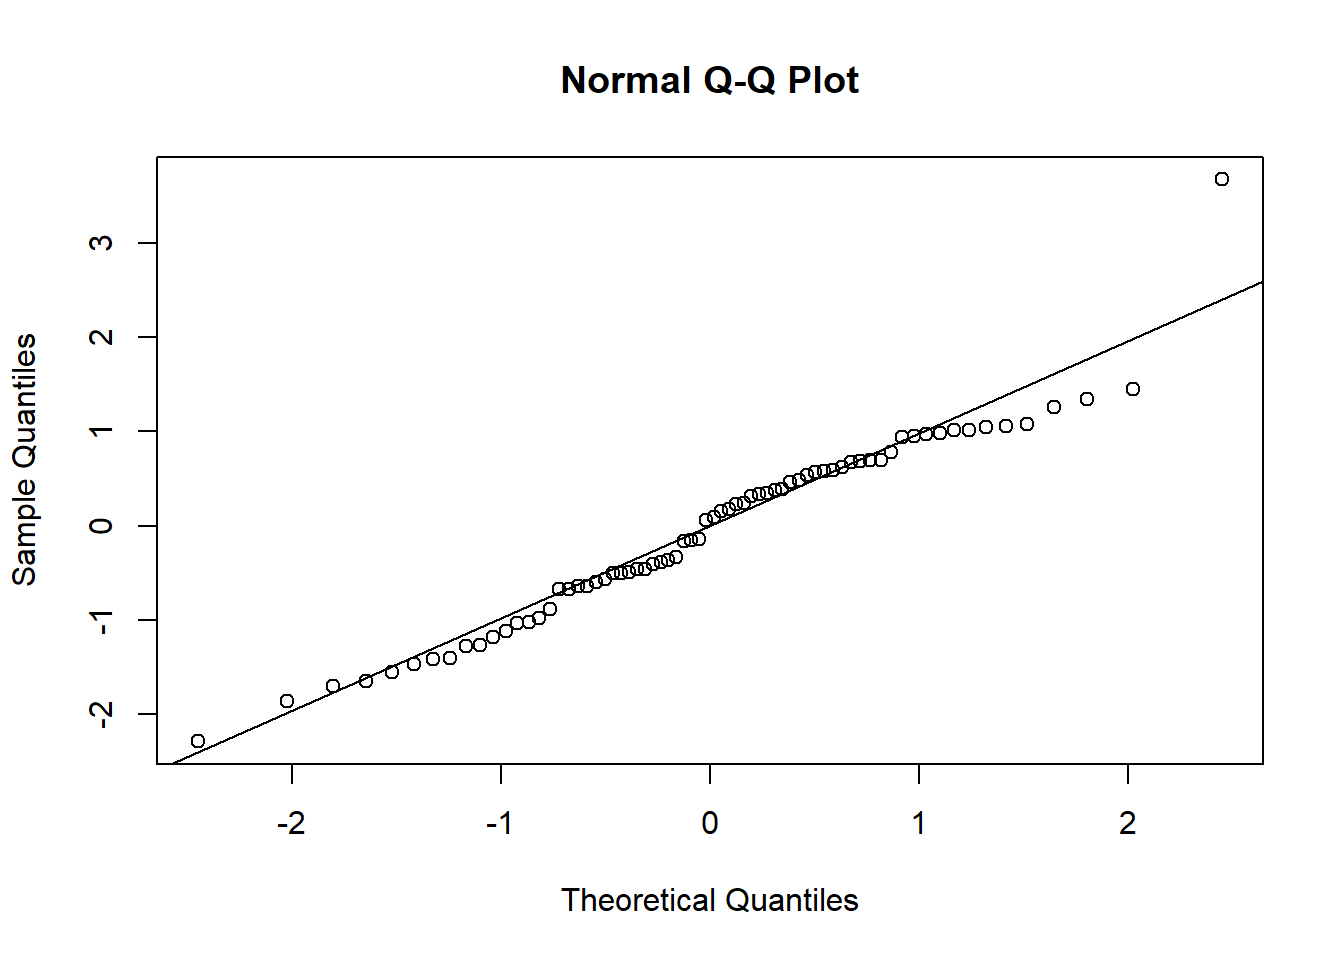
\includegraphics{GLMM_files/figure-latex/unnamed-chunk-5-1.pdf}

\begin{Shaded}
\begin{Highlighting}[]
\FunctionTok{shapiro.test}\NormalTok{(deviance.resids)}
\end{Highlighting}
\end{Shaded}

\begin{verbatim}
## 
##  Shapiro-Wilk normality test
## 
## data:  deviance.resids
## W = 0.96065, p-value = 0.02719
\end{verbatim}

\begin{Shaded}
\begin{Highlighting}[]
\FunctionTok{hist}\NormalTok{(deviance.resids, }\AttributeTok{freq =} \ConstantTok{FALSE}\NormalTok{)}
\NormalTok{dev.norm }\OtherTok{\textless{}{-}} \ControlFlowTok{function}\NormalTok{(x) }\FunctionTok{dnorm}\NormalTok{(x,}\FunctionTok{mean}\NormalTok{(deviance.resids), }\FunctionTok{sd}\NormalTok{(deviance.resids))}
\FunctionTok{curve}\NormalTok{(dev.norm, }\SpecialCharTok{{-}}\DecValTok{5}\NormalTok{,}\DecValTok{5}\NormalTok{, }\AttributeTok{add =} \ConstantTok{TRUE}\NormalTok{)}
\end{Highlighting}
\end{Shaded}

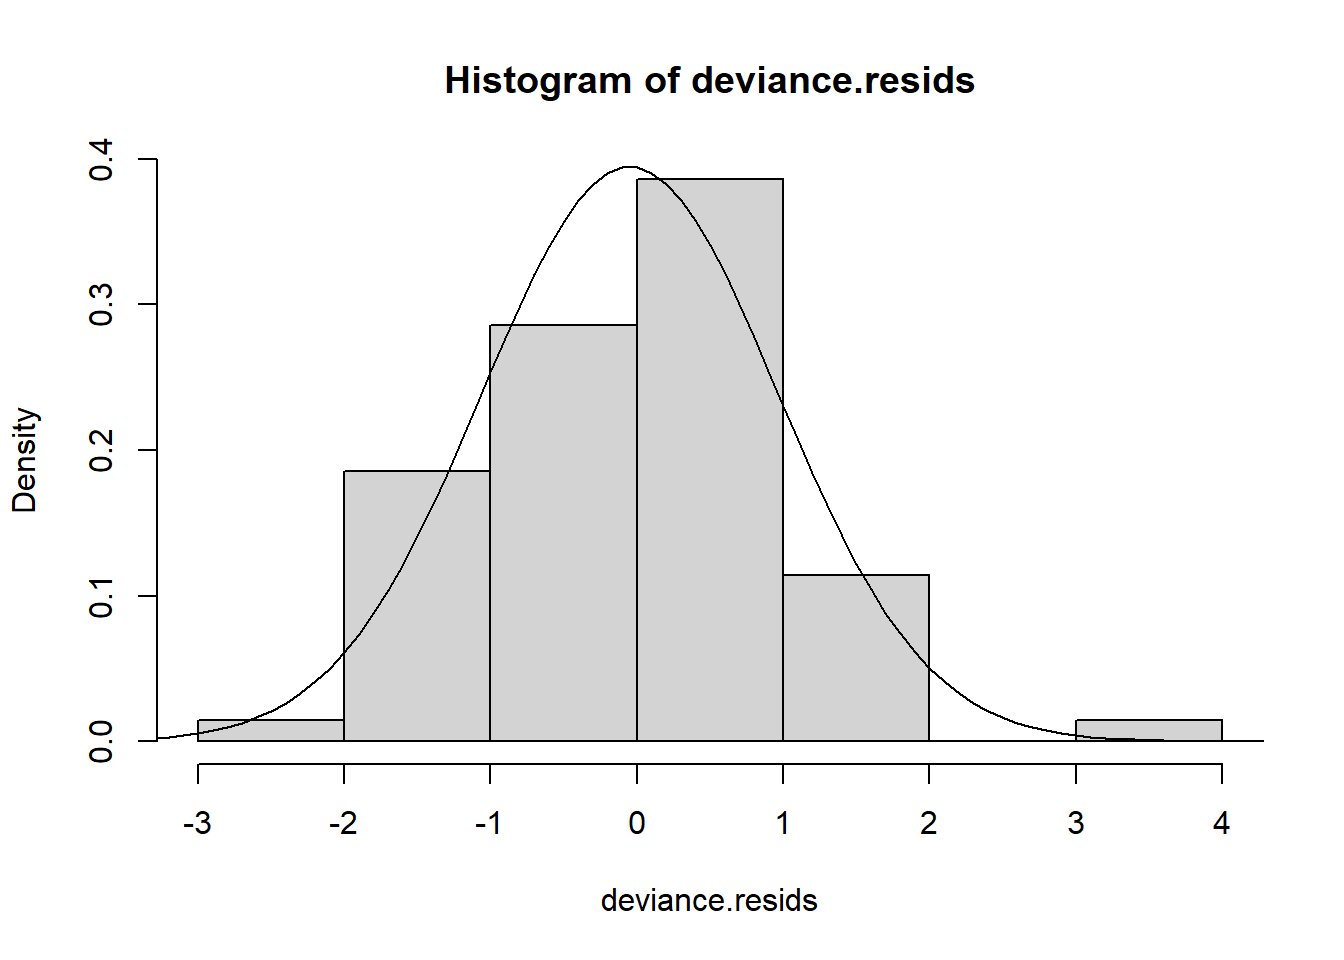
\includegraphics{GLMM_files/figure-latex/unnamed-chunk-5-2.pdf}

\begin{Shaded}
\begin{Highlighting}[]
\FunctionTok{plot}\NormalTok{(mu, deviance.resids)}
\end{Highlighting}
\end{Shaded}

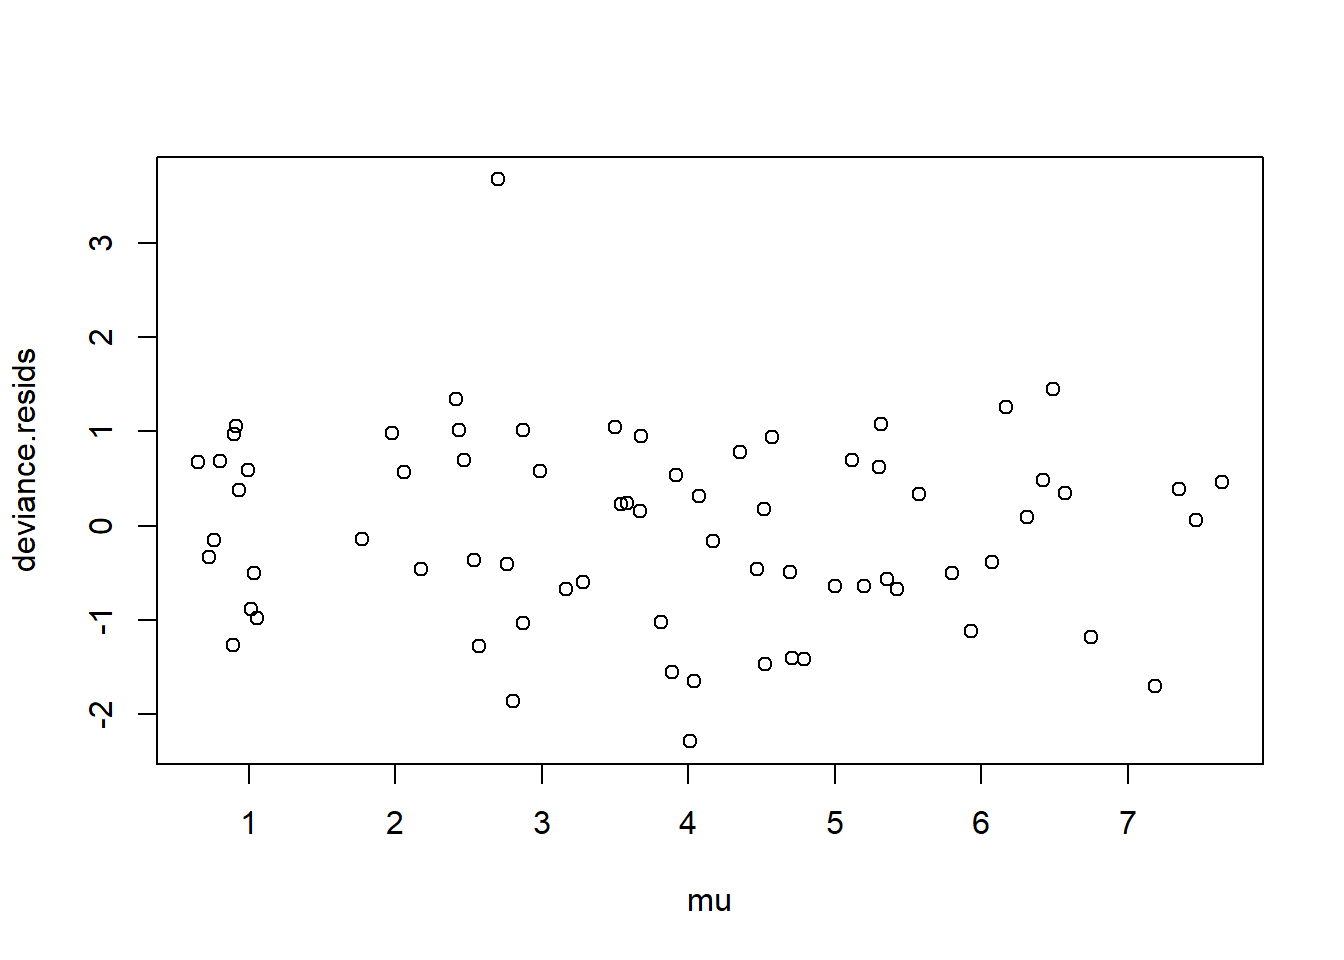
\includegraphics{GLMM_files/figure-latex/unnamed-chunk-5-3.pdf}

\begin{Shaded}
\begin{Highlighting}[]
\CommentTok{\# residual plots using pearson residuals}
\FunctionTok{qqnorm}\NormalTok{(pearson.resids)}
\FunctionTok{qqline}\NormalTok{(pearson.resids)}
\end{Highlighting}
\end{Shaded}

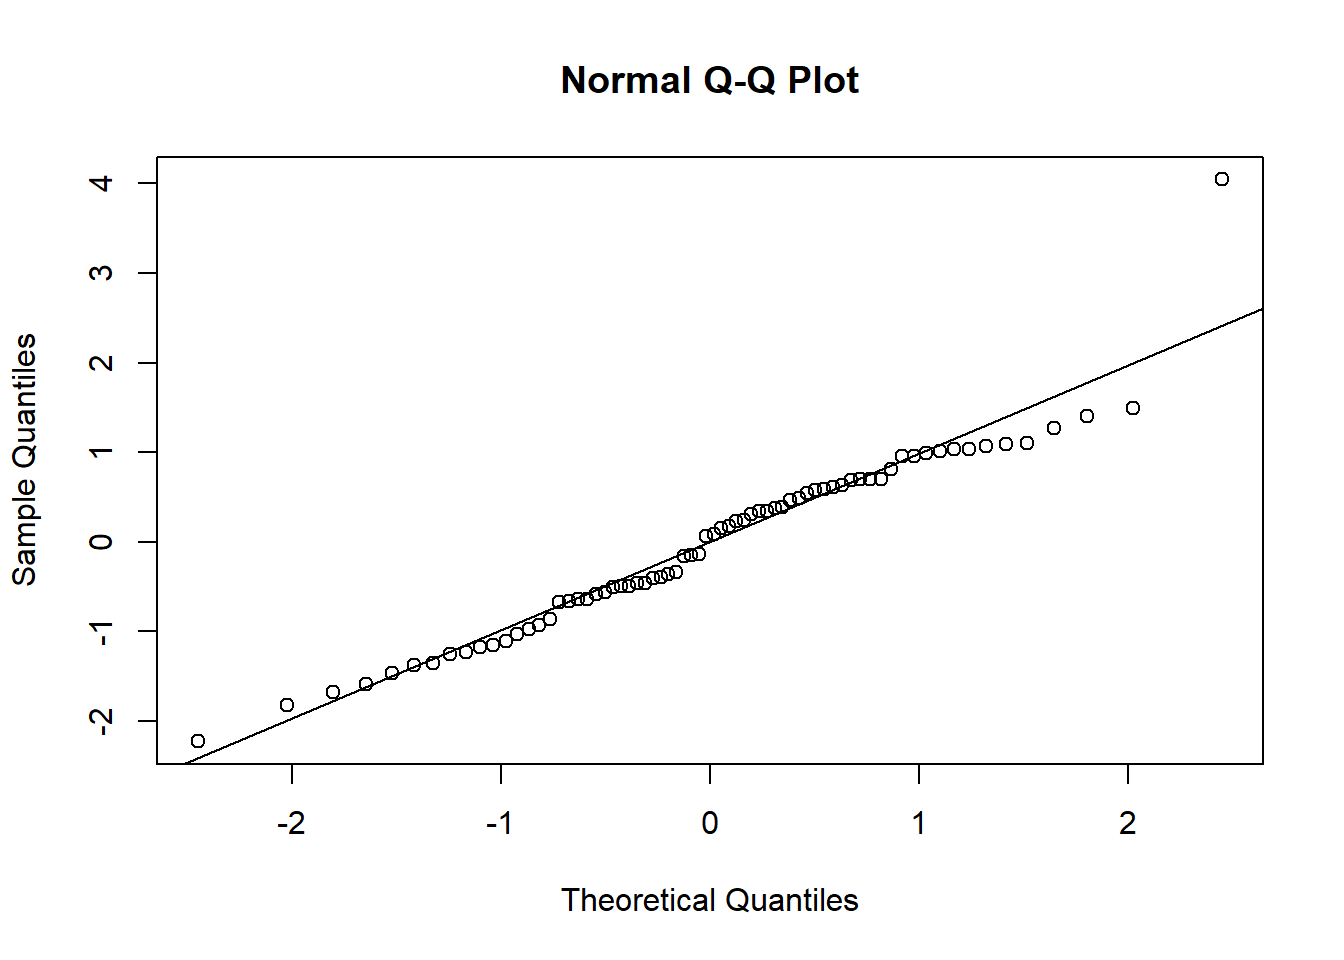
\includegraphics{GLMM_files/figure-latex/unnamed-chunk-5-4.pdf}

\begin{Shaded}
\begin{Highlighting}[]
\FunctionTok{shapiro.test}\NormalTok{(pearson.resids)}
\end{Highlighting}
\end{Shaded}

\begin{verbatim}
## 
##  Shapiro-Wilk normality test
## 
## data:  pearson.resids
## W = 0.94988, p-value = 0.007147
\end{verbatim}

\begin{Shaded}
\begin{Highlighting}[]
\FunctionTok{hist}\NormalTok{(pearson.resids, }\AttributeTok{freq =} \ConstantTok{FALSE}\NormalTok{)}
\NormalTok{pearson.norm }\OtherTok{\textless{}{-}} \ControlFlowTok{function}\NormalTok{(x) }\FunctionTok{dnorm}\NormalTok{(x,}\FunctionTok{mean}\NormalTok{(pearson.resids), }\FunctionTok{sd}\NormalTok{(pearson.resids))}
\FunctionTok{curve}\NormalTok{(pearson.norm, }\SpecialCharTok{{-}}\DecValTok{5}\NormalTok{,}\DecValTok{5}\NormalTok{, }\AttributeTok{add =} \ConstantTok{TRUE}\NormalTok{)}
\end{Highlighting}
\end{Shaded}

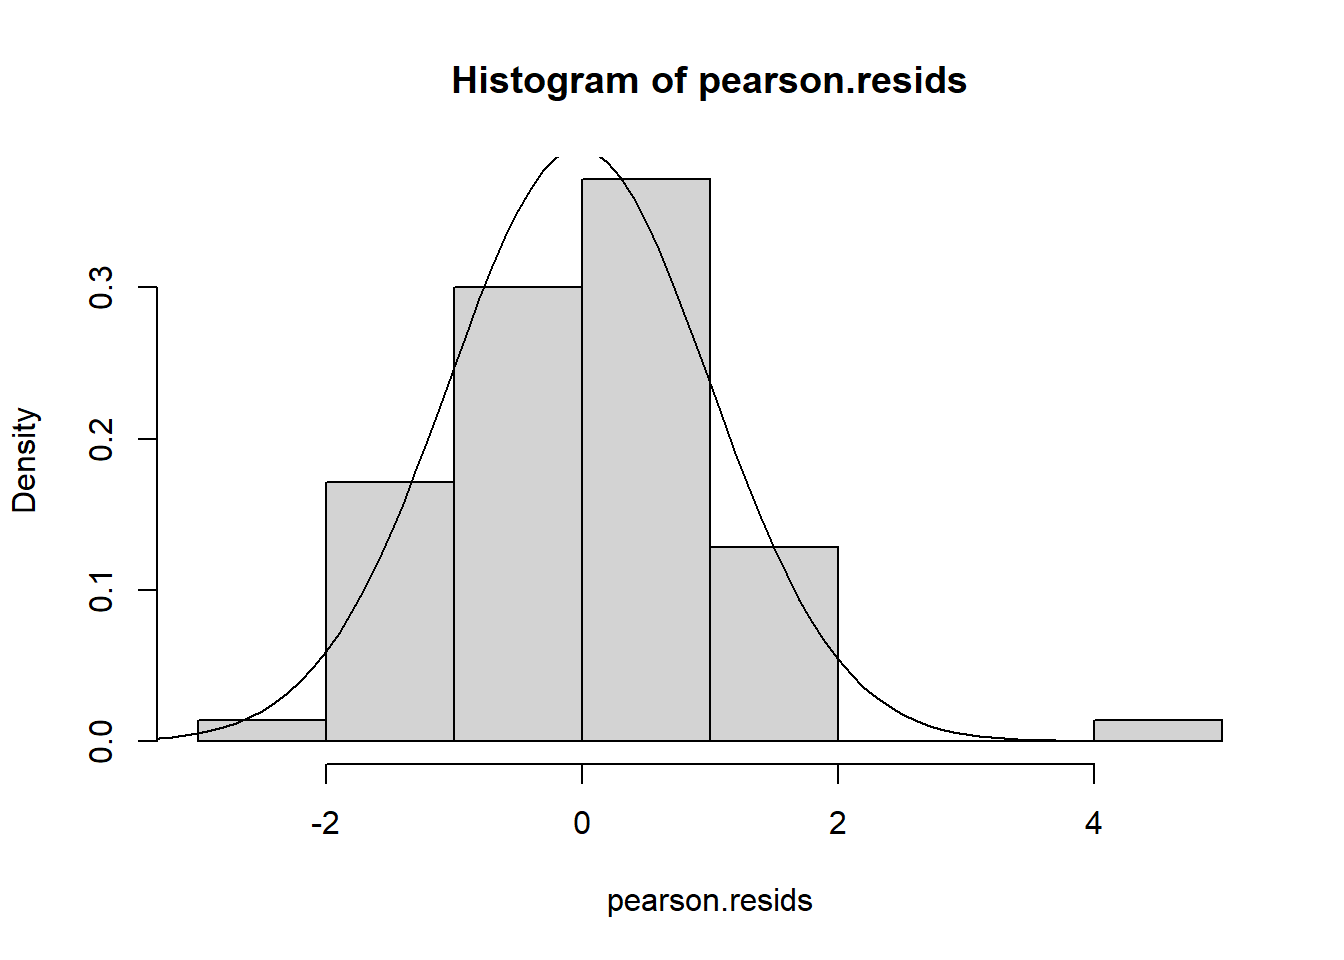
\includegraphics{GLMM_files/figure-latex/unnamed-chunk-5-5.pdf}

\begin{Shaded}
\begin{Highlighting}[]
\FunctionTok{plot}\NormalTok{(mu, pearson.resids)}
\end{Highlighting}
\end{Shaded}

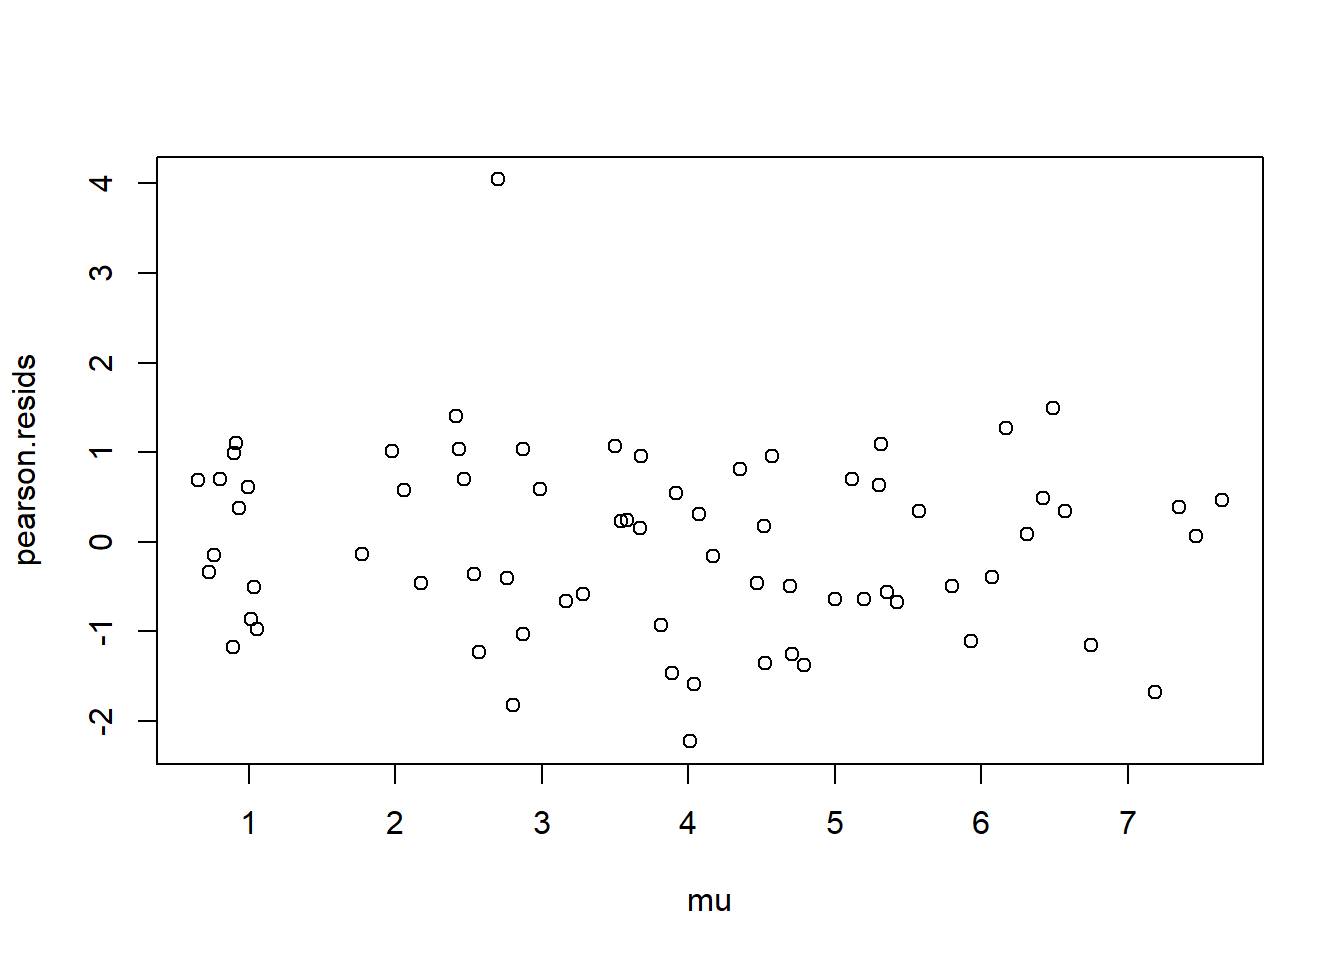
\includegraphics{GLMM_files/figure-latex/unnamed-chunk-5-6.pdf}

\begin{Shaded}
\begin{Highlighting}[]
\CommentTok{\# plots are using what look like Pearson (or maybe deviance) residuals versus predicted values under canonical link, i.e. log(Y hat)}
\FunctionTok{plot}\NormalTok{(}\FunctionTok{log}\NormalTok{(group.sizes}\SpecialCharTok{*}\NormalTok{mu), pearson.resids)}
\end{Highlighting}
\end{Shaded}

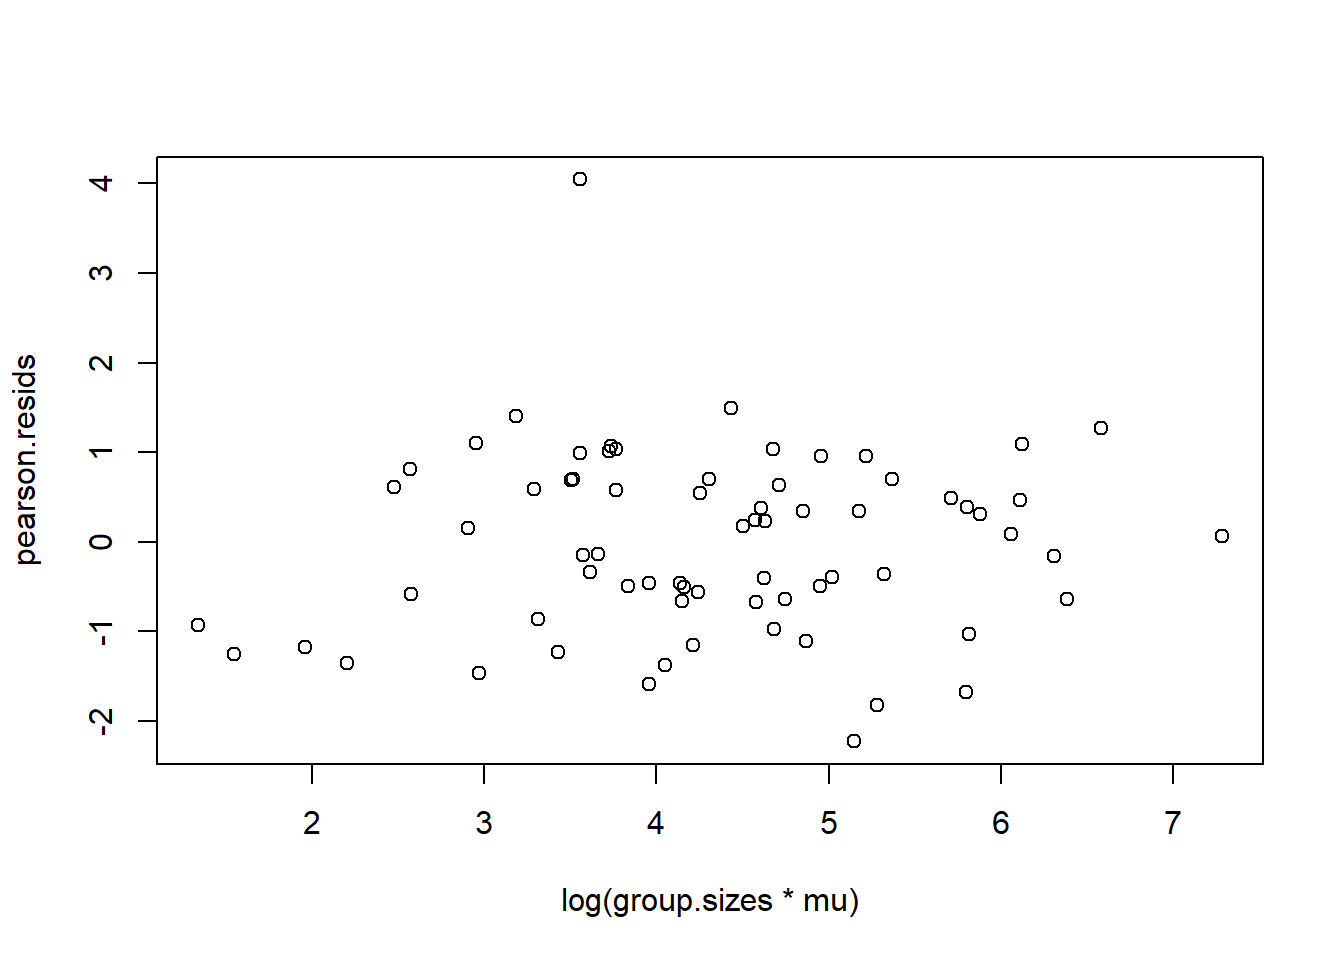
\includegraphics{GLMM_files/figure-latex/unnamed-chunk-5-7.pdf}

\begin{Shaded}
\begin{Highlighting}[]
\FunctionTok{plot}\NormalTok{(my.glm)}
\end{Highlighting}
\end{Shaded}

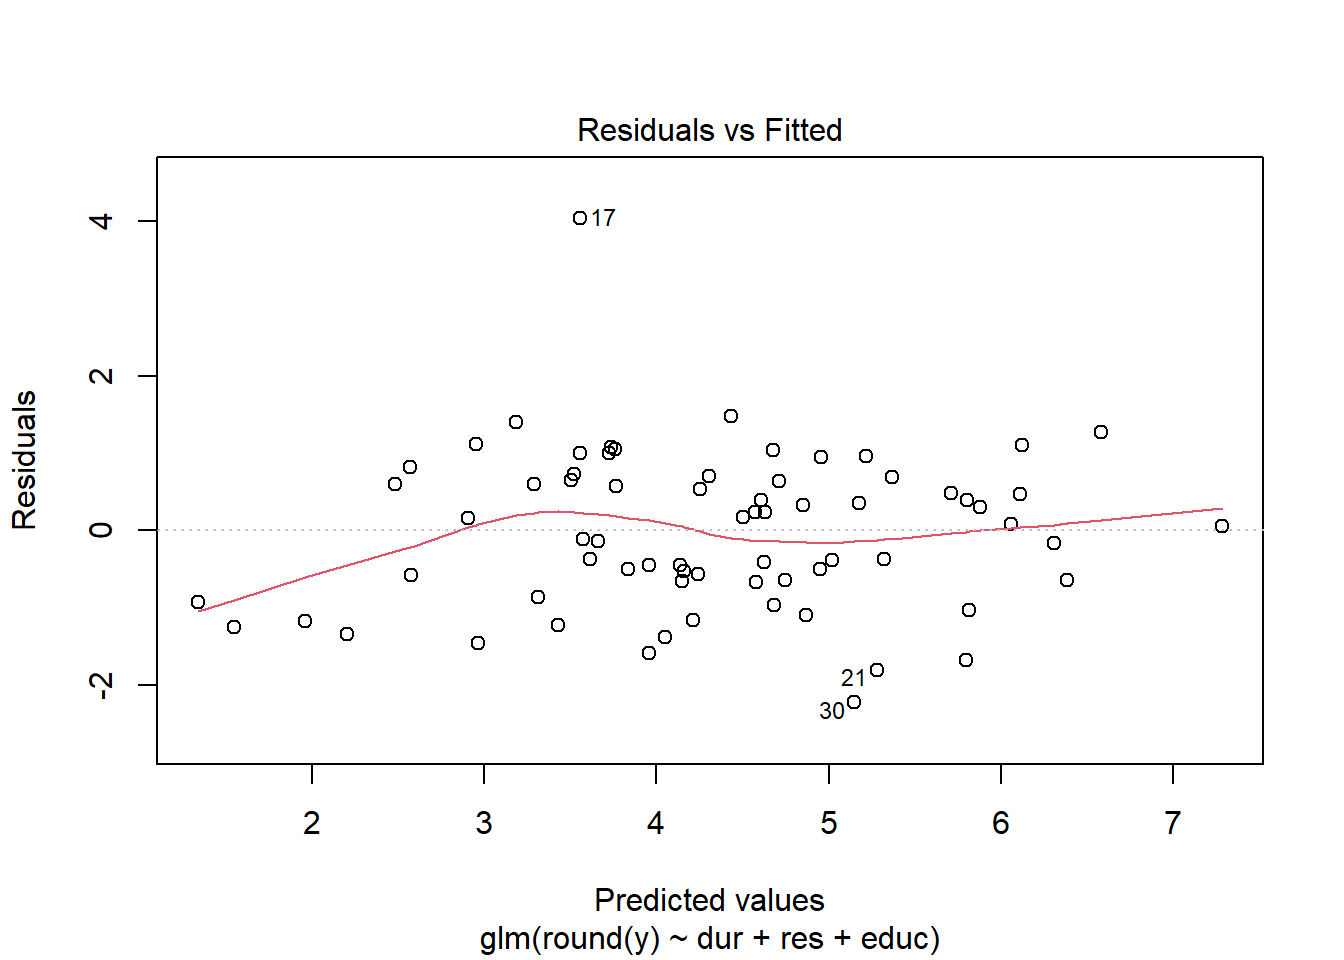
\includegraphics{GLMM_files/figure-latex/unnamed-chunk-5-8.pdf} 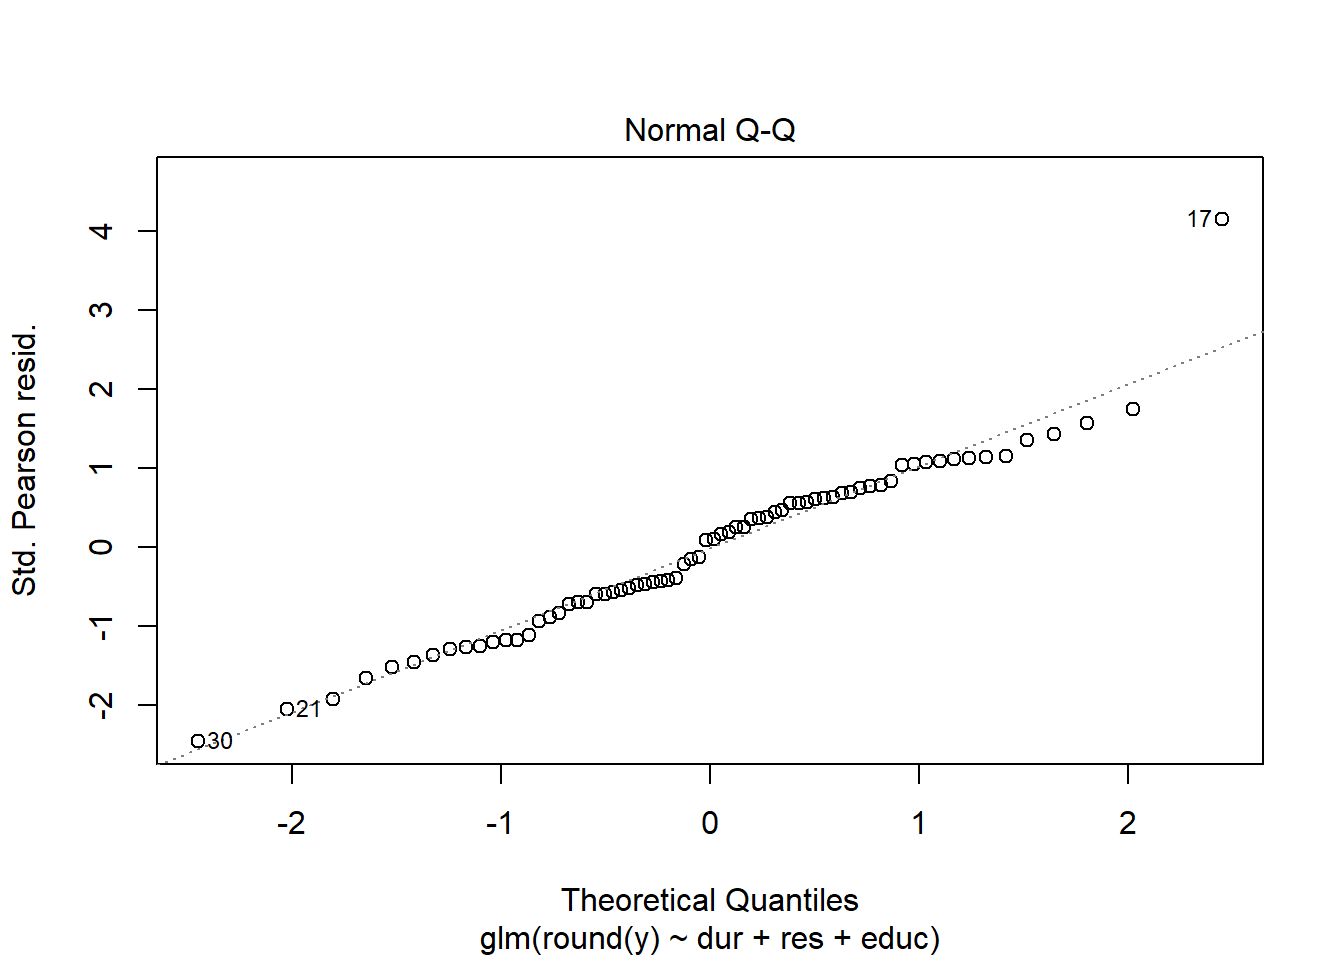
\includegraphics{GLMM_files/figure-latex/unnamed-chunk-5-9.pdf} 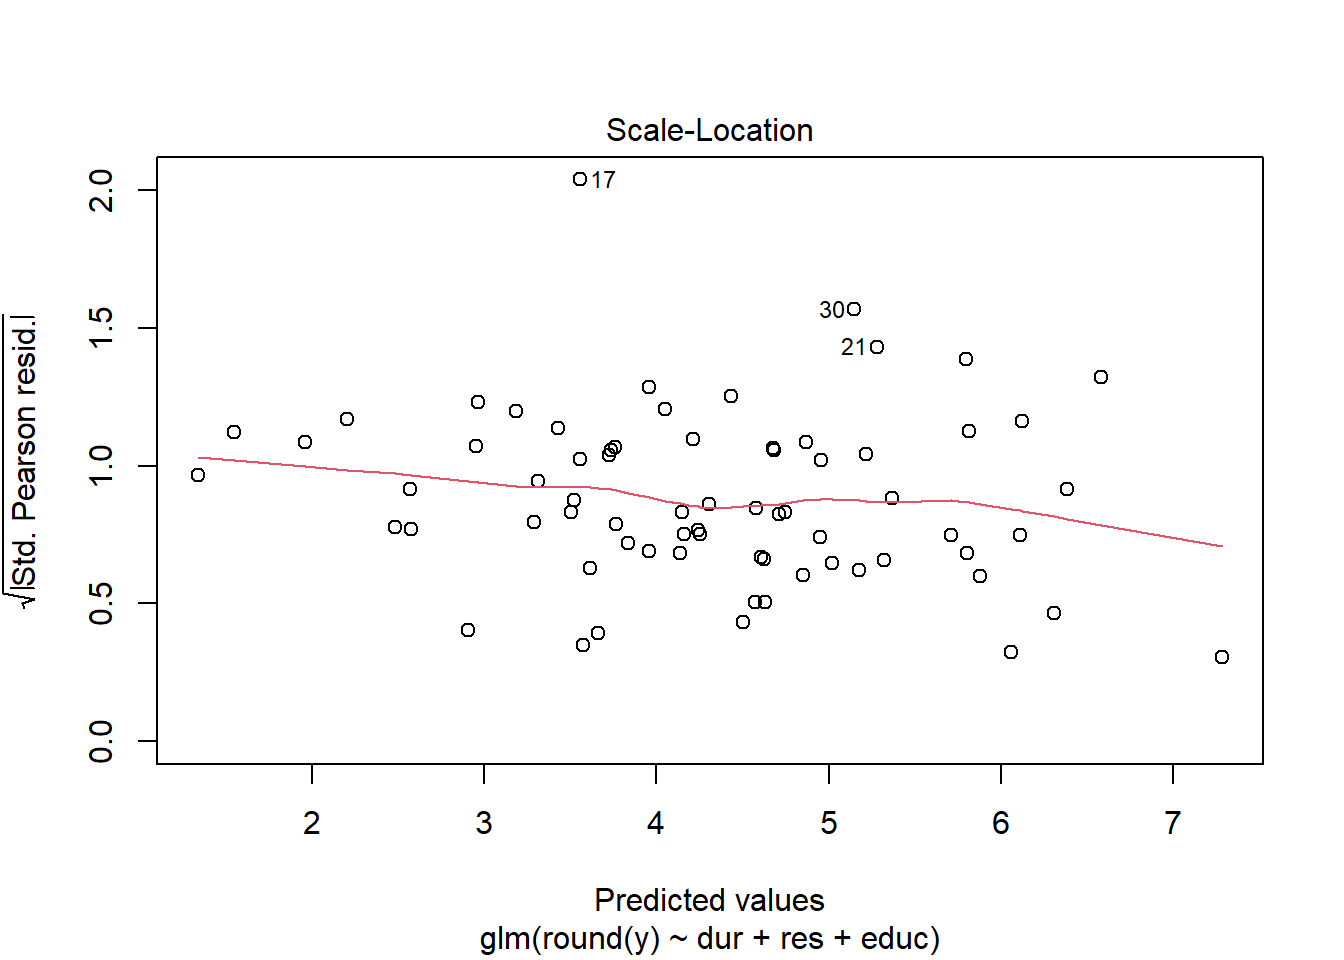
\includegraphics{GLMM_files/figure-latex/unnamed-chunk-5-10.pdf} 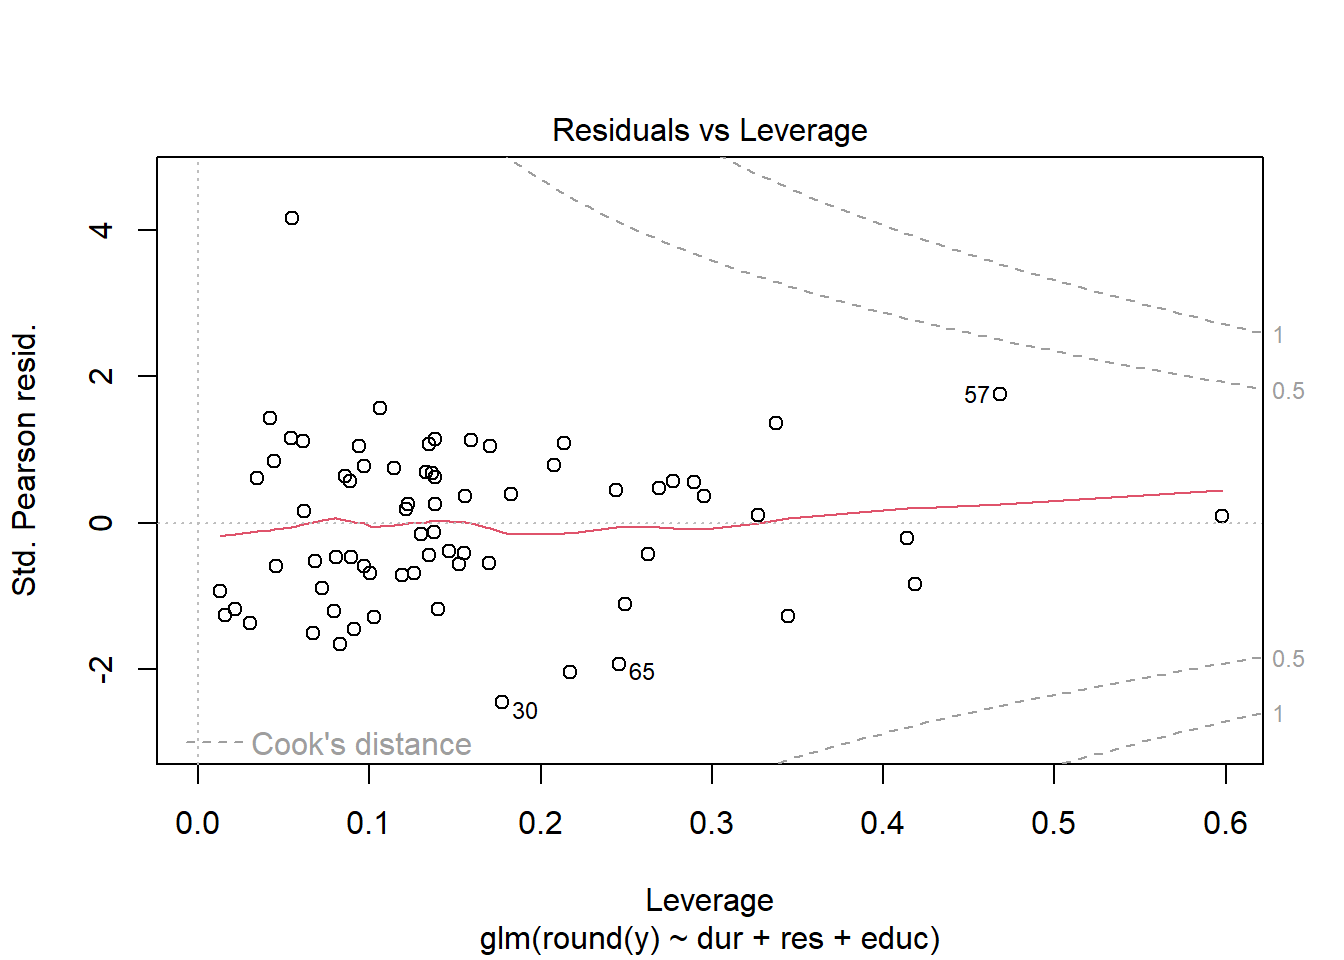
\includegraphics{GLMM_files/figure-latex/unnamed-chunk-5-11.pdf}

\hypertarget{outlier-analysis-using-cooks-distance}{%
\section{Outlier analysis using Cook's distance}\label{outlier-analysis-using-cooks-distance}}

Outliers are observations corresponding to large residuals. They may occur due to chance, or, more likely, indicate a lack of model fit for a specific observation. The lack of fit may be due to something innocuous like a mistake made in recording data; or, it may be that the observation in question is very different from the others in the sample, and does not follow the same response-covariate relationship.

Outliers are not a problem, however, unless their inclusion causes the fitted model to be substantially different than had they been excluded. Therefore, we do not necessarily care that a particular residual is large, but that it is influential on the model fit.

In multiple linear regression we may measure this influence by Cook's distance of the data point, which is related to both the magnitude of its residual and its leverage, as measured by the hat (or influence) matrix. For GLMs we can define the Cook's distance in the same manner: the Cook's distance of data point \(k\) is given by
\[C_k = \frac{1}{(p+1)}\sum_{i=1}^n \frac{(\hat\mu_i^{[k]} - \hat\mu_i)^2}{\hat\phi V(\hat\mu_i)}; \text{ or}\]
\[C_k = \frac{(e^P_k)^2}{\hat\phi (p+1)}\frac{h_k}{(1-h_k)^2}\]
where \(H = W^{1/2}X(X^\top W X)^{-1}X^\top W^{1/2}\) is the hat matrix and \(h_k\) is its \(k^{th}\) diagonal entry. Large Cook's distance implies the model predictions change substantially when the data point in question is removed.

\hypertarget{outlier-analysis-for-the-ceb-data}{%
\subsection{Outlier analysis for the CEB data}\label{outlier-analysis-for-the-ceb-data}}

Typically data points with Cook's distance \(>1\) are considered highly influential and the case for their exclusion is considerable. In this case, our apparent outlier is not influential, nor is it even the most influential observation sampled.

Below we have computed Cook's distance ``by hand'' and by using the corresponding built-in R function; the only (very slight) difference between the two seems to be caused by the fact the built-in function uses the glm object, which we fitted after rounding the responses, whereas our ``by hand'' calculation uses Pearson residuals based on the original (unrounded) responses.

\begin{Shaded}
\begin{Highlighting}[]
\NormalTok{ceb2 }\OtherTok{\textless{}{-}}\NormalTok{ ceb[}\SpecialCharTok{{-}}\DecValTok{17}\NormalTok{,]}
\NormalTok{my.glm2 }\OtherTok{\textless{}{-}} \FunctionTok{glm}\NormalTok{(}\FunctionTok{round}\NormalTok{(y)}\SpecialCharTok{\textasciitilde{}}\NormalTok{dur}\SpecialCharTok{+}\NormalTok{res}\SpecialCharTok{+}\NormalTok{educ, }\AttributeTok{family =} \FunctionTok{poisson}\NormalTok{(}\AttributeTok{link =} \StringTok{\textquotesingle{}log\textquotesingle{}}\NormalTok{), }\AttributeTok{data =}\NormalTok{ ceb2, }\AttributeTok{offset =} \FunctionTok{log}\NormalTok{(n))}

\NormalTok{W2 }\OtherTok{\textless{}{-}} \FunctionTok{sqrt}\NormalTok{(W)}
\NormalTok{h }\OtherTok{\textless{}{-}}\NormalTok{ W2}\SpecialCharTok{\%*\%}\NormalTok{X}\SpecialCharTok{\%*\%}\FunctionTok{solve}\NormalTok{(}\FunctionTok{t}\NormalTok{(X)}\SpecialCharTok{\%*\%}\NormalTok{W}\SpecialCharTok{\%*\%}\NormalTok{X)}\SpecialCharTok{\%*\%}\FunctionTok{t}\NormalTok{(X)}\SpecialCharTok{\%*\%}\NormalTok{W2}

\NormalTok{((pearson.resids[}\DecValTok{17}\NormalTok{]}\SpecialCharTok{\^{}}\DecValTok{2}\NormalTok{)}\SpecialCharTok{/}\NormalTok{p)}\SpecialCharTok{*}\NormalTok{(h[}\DecValTok{17}\NormalTok{,}\DecValTok{17}\NormalTok{]}\SpecialCharTok{/}\NormalTok{((}\DecValTok{1}\SpecialCharTok{{-}}\NormalTok{h[}\DecValTok{17}\NormalTok{,}\DecValTok{17}\NormalTok{])}\SpecialCharTok{\^{}}\DecValTok{2}\NormalTok{))}
\end{Highlighting}
\end{Shaded}

\begin{verbatim}
## [1] 0.0912897
\end{verbatim}

\begin{Shaded}
\begin{Highlighting}[]
\NormalTok{cd }\OtherTok{\textless{}{-}} \FunctionTok{cooks.distance}\NormalTok{(my.glm)}

\NormalTok{cd[}\DecValTok{17}\NormalTok{]}
\end{Highlighting}
\end{Shaded}

\begin{verbatim}
##         17 
## 0.09123744
\end{verbatim}

\begin{Shaded}
\begin{Highlighting}[]
\FunctionTok{sort}\NormalTok{(cd)}
\end{Highlighting}
\end{Shaded}

\begin{verbatim}
##           44           12           16           43           58           26 
## 0.0001578983 0.0002173653 0.0003181272 0.0004391595 0.0004872775 0.0008276467 
##           31           48           69            5           40           37 
## 0.0009604834 0.0010416260 0.0011600877 0.0011813567 0.0015364693 0.0017374273 
##           63           15           59           64            8           18 
## 0.0017913034 0.0020157684 0.0022231406 0.0023307859 0.0024333875 0.0027257717 
##            1           29           54           56           34           62 
## 0.0027795217 0.0028483882 0.0029171612 0.0029318194 0.0030296972 0.0030322783 
##           55           36           27           33            9           60 
## 0.0033869538 0.0034063422 0.0048780994 0.0049440311 0.0052402581 0.0053485413 
##           47            6           24            3           11           23 
## 0.0055965679 0.0056512722 0.0056712755 0.0057553959 0.0059235574 0.0061112712 
##           50           41           14           49            4            2 
## 0.0062842199 0.0063288779 0.0064608723 0.0067079644 0.0067366794 0.0068678049 
##           66           25           13            7           61           71 
## 0.0072889100 0.0074308461 0.0082351514 0.0104259702 0.0110105154 0.0114006236 
##           70           42           52           20           28           32 
## 0.0115384460 0.0145603375 0.0149361729 0.0164709118 0.0173145140 0.0189913643 
##           51           38           53           19           39           67 
## 0.0191422888 0.0203317679 0.0205784895 0.0220776790 0.0225077753 0.0265192825 
##           35           10           45           22           46           17 
## 0.0290870153 0.0375227510 0.0462157923 0.0771290592 0.0847041708 0.0912374357 
##           21           65           30           57 
## 0.1058278940 0.1102296604 0.1184297114 0.2448544534
\end{verbatim}

\hypertarget{linear-mixed-models}{%
\chapter{Linear Mixed Models}\label{linear-mixed-models}}

\hypertarget{anova-with-random-factors}{%
\section{ANOVA with random factors}\label{anova-with-random-factors}}

The simplest linear mixed models are used to analyze linear models for one-way ANOVA, randomized complete block designs, and two-way ANOVA. \emph{Mixed} models as opposed to \emph{fixed} models (the linear models you have heretofore studied) are needed when factors have levels that are \textbf{random}. Random levels occur whenever the units making up those levels behave like random samples from a population. Two examples are given below. And, we discuss how to perform ANOVA-like tests for factors that are random rather than fixed. The upshot is that (at least for balanced experiments/datasets) the tests for fixed effects are identical to those for random effects, only the interpretation is different (and importantly so!).

\hypertarget{strength-of-metallic-bonds}{%
\subsection{Strength of metallic bonds}\label{strength-of-metallic-bonds}}

The dataset below, called ``Bonds'', contains responses for 21 samples of metals, 7 each for iron, nickel, and copper, that quantify the strength of metallic bonds. One sample from each metal was extracted from each of 7 ingots. We expect ingots to act like blocks---differences in ingots account for a substantial amount of variability in the responses, but the precise block effects are of no inferential/scientific inference. We only include the blocks in order to reduce the residual variance after accounting for block variance. A randomized controlled block design describes how this data was collected, but, if we repeated the experiment, the blocks (ingots) would be completely different. That is, the blocks are not \emph{fixed} but \emph{random}. Rather than estimating block effects that would surely change experiment to experiment, we should focus on estimating the amount of variability explained by the blocks, which should remain about the same experiment to experiment. This suggests a different model than used to analyze RCBD experiments with fixed blocks.

The usual linear model for fixed blocks is
\[y_{ijk} = \mu + \alpha_i + \beta_j + \epsilon_{ij},\]
where \(y_{ij}\) is the response for treatment (metal) \(i\) in block (ingot) \(j\); the \(\alpha_i\)'s are the metal (treatment) effects; the \(\beta_j\)'s are the ingot (block) effects; and, \(\epsilon_{ij}\stackrel{iid}{\sim}N(0,\sigma^2)\) are the random residuals.

The above linear model is the wrong model for this data because the block effects (and, hence, also the interaction effects) are meaningless outside of the given data set; these are not population-level parameters because the blocks are random rather than fixed. The appropriate model (given normality and independence of random residuals is reasonable) is the following \emph{mixed effects model}:

\begin{equation}
y_{ij} = \mu + \alpha_i + \beta_j + \epsilon_{ij},
 \label{eq:fullmodel}
\end{equation}
where \(\beta_j\stackrel{iid}{\sim}N(0, \sigma_b^2)\) and, independently, \(\epsilon_{ij}\stackrel{iid}{\sim}N(0,\sigma^2)\).

For \emph{balanced} experiments (the number of replicates is equal across each combination of factor levels) we can test for block and treatment effects by comparing nested/aggregated models. Let \(\overline Y_{i\cdot}\) denote the mean response for metal \(i\) averaged over ingots. We can write down the following aggregated model from \eqref{eq:fullmodel} as
\begin{equation}
\overline y_{i\cdot} = \mu + \alpha_i + \epsilon_{i},
 \label{eq:aggmodel1}
\end{equation}
where \(\epsilon_i = \frac{1}{J}\sum_{j=1}^j \epsilon_{ij}\). Then, \(\epsilon_j\) has variance \(\sigma_b^2 + \sigma^2/J\). The F statistic
\[F = \frac{J\cdot MSE_{agg}}{MSE_{full}}\]
where \(MSE_{agg}\) and \(MSE_{full}\) are the mean squared errors from the models in \eqref{eq:aggmodel1} and \eqref{eq:fullmodel} can be used to test the hypothesis \(H_0:\sigma_b^2 = 0\).

\hypertarget{machine-productivity}{%
\subsection{Machine productivity}\label{machine-productivity}}

The dataset given below contains the results of a designed experiment to evaluate worker productivity using 3 different industrial machines. The goal is to determine which machine is most productive while controlling for natural variation in worker productivity. The observed workers represent a random sample from a population of workers (blocks), analogous to the ingots in the previous example. The difference between the two examples (besides the context) is that the machine treatments are replicated wihtin workers, so that there are three observations of a productivity score fore each worker for each type of machine. This means that we can fit a model with \emph{interaction terms} capable of capturing changes in machine effects on productivity between different workers (if those changes are present):
\begin{equation}
y_{ijk} = \mu + \alpha_i + \beta_j + (\alpha\beta)_{ij} + \epsilon_{ijk},
 \label{eq:fullmodel2}
\end{equation}
where \(k\) denotes the \(k^{\text{th}}\) replicate within machine \(i\) and worker \(j\); and where \((\alpha\beta)_{ij}\) denote the machine-worker interaction effects.

Let \(\overline Y_{ij\cdot}\) be the mean response averaging over replicates for the treatment \(i\) and block \(j\) combination. Then,
\begin{align*}
V(\overline Y_{ij\cdot}) &= V\left(K^{-1}\sum_{k=1}^K Y_{ijk}\right) \\
&= \frac{1}{K^2}V\left(\sum_{k=1}^K \{\mu+\alpha_i+\beta_j + (\alpha\beta)_{ij} + \epsilon_{ijk}\}\right)\\
& = \frac{1}{K^2}V\left(K\mu + K\alpha_i + K\beta_j + K(\alpha\beta)_{ij} + \sum_{k=1}^K \epsilon_{ijk}\right)\\
& = \sigma_b^2 + \sigma_{ab}^2 + K^{-1}\sigma^2.
\end{align*}
If we rewrite the model for the cell mean responses as
\begin{equation}
\overline y_{ij\cdot} = \mu + \alpha_i + \beta_j + \epsilon_{ij},
 \label{eq:aggmodel}
\end{equation}
then the aggregated error term follows \(\epsilon_{ij}\stackrel{iid}{\sim}N(0, \sigma_{ab}^2 + \sigma^2/K)\). The residual mean square (or called the mean squared error) of model \eqref{eq:fullmodel2} (let's call it \(MSE_{\text{full}}\)) has mean \(\sigma^2\) with \(n-p_1\) degrees of freedom where \(n\) is the sample size and \(p\) is the number of coefficients in the fitted model (\(p_1\) equals the number of crossed factor levels, the number of blocks times the number of treatments). The residual mean square for the aggregated model in \eqref{eq:aggmodel} (let's call it \(MSE_{\text{agg}}\)) has mean \(\sigma_{ab}^2 + \sigma^2/K\) with \(n/K-p_2\) degrees of freedom where \(p_2\) is the number of treatments plus the number of blocks minus 1. An unbiased estimate of \(\sigma_{ab}^2\) is given by \(MSE_{\text{agg}} - \frac{1}{K}MSE_{\text{full}}\). Consider testing the null hypothesis \(H_0:\sigma_{ab}^2 = 0\). The statistic
\[F := \frac{K\cdot MSE_{agg}}{MSE_{full}}\stackrel{H_0}{\sim}F_{n/K-p_2, n-p_1},\]
that is, under the null hypothesis. The test that rejects \(H_0\) for \(F > F_{1-\alpha,n/K-p_2, n-p_1}\) is exactly equivalent to the partial F test between the full model and the full model without the interaction terms (the additive model).

Below we use R to compute ANOVA tables for the full model, full model without interaction, and the aggregated model. The F test statistic for the aggregated model is about 46.13 on 10 and 36 degrees of freedom, which exactly matches the partial F test between the full and additive models.

\begin{Shaded}
\begin{Highlighting}[]
\FunctionTok{library}\NormalTok{(nlme)}

\CommentTok{\# aggregated model}
\NormalTok{Mach.agg }\OtherTok{\textless{}{-}} \FunctionTok{aggregate}\NormalTok{(score}\SpecialCharTok{\textasciitilde{}}\NormalTok{Machine}\SpecialCharTok{*}\NormalTok{Worker, }\AttributeTok{data =}\NormalTok{ Machines, }\AttributeTok{FUN=}\NormalTok{mean)}

\NormalTok{m2 }\OtherTok{\textless{}{-}} \FunctionTok{lm}\NormalTok{(score}\SpecialCharTok{\textasciitilde{}}\NormalTok{Machine}\SpecialCharTok{+}\NormalTok{Worker, }\AttributeTok{data =}\NormalTok{ Mach.agg)}

\FunctionTok{anova}\NormalTok{(m2)}
\end{Highlighting}
\end{Shaded}

\begin{verbatim}
## Analysis of Variance Table
## 
## Response: score
##           Df Sum Sq Mean Sq F value    Pr(>F)    
## Machine    2 585.09 292.544 20.5761 0.0002855 ***
## Worker     5 413.97  82.793  5.8232 0.0089495 ** 
## Residuals 10 142.18  14.218                      
## ---
## Signif. codes:  0 '***' 0.001 '**' 0.01 '*' 0.05 '.' 0.1 ' ' 1
\end{verbatim}

\begin{Shaded}
\begin{Highlighting}[]
\CommentTok{\# full model with interaction}
\NormalTok{m0 }\OtherTok{\textless{}{-}} \FunctionTok{lm}\NormalTok{(score}\SpecialCharTok{\textasciitilde{}}\NormalTok{Machine}\SpecialCharTok{*}\NormalTok{Worker, }\AttributeTok{data =}\NormalTok{ Machines)}

\FunctionTok{anova}\NormalTok{(m0)}
\end{Highlighting}
\end{Shaded}

\begin{verbatim}
## Analysis of Variance Table
## 
## Response: score
##                Df  Sum Sq Mean Sq F value    Pr(>F)    
## Machine         2 1755.26  877.63  949.17 < 2.2e-16 ***
## Worker          5 1241.89  248.38  268.63 < 2.2e-16 ***
## Machine:Worker 10  426.53   42.65   46.13 < 2.2e-16 ***
## Residuals      36   33.29    0.92                      
## ---
## Signif. codes:  0 '***' 0.001 '**' 0.01 '*' 0.05 '.' 0.1 ' ' 1
\end{verbatim}

\begin{Shaded}
\begin{Highlighting}[]
\NormalTok{(}\FloatTok{142.18}\SpecialCharTok{*}\DecValTok{3}\SpecialCharTok{/}\DecValTok{10}\NormalTok{)}\SpecialCharTok{/}\NormalTok{(}\FloatTok{33.29}\SpecialCharTok{/}\DecValTok{36}\NormalTok{)}
\end{Highlighting}
\end{Shaded}

\begin{verbatim}
## [1] 46.12628
\end{verbatim}

\begin{Shaded}
\begin{Highlighting}[]
\DecValTok{1}\SpecialCharTok{{-}}\FunctionTok{pf}\NormalTok{((}\FloatTok{142.18}\SpecialCharTok{*}\DecValTok{3}\SpecialCharTok{/}\DecValTok{10}\NormalTok{)}\SpecialCharTok{/}\NormalTok{(}\FloatTok{33.29}\SpecialCharTok{/}\DecValTok{36}\NormalTok{), }\DecValTok{10}\NormalTok{, }\DecValTok{36}\NormalTok{)}
\end{Highlighting}
\end{Shaded}

\begin{verbatim}
## [1] 0
\end{verbatim}

\begin{Shaded}
\begin{Highlighting}[]
\CommentTok{\# additive model (no interaction)}
\NormalTok{m1 }\OtherTok{\textless{}{-}} \FunctionTok{lm}\NormalTok{(score}\SpecialCharTok{\textasciitilde{}}\NormalTok{Machine}\SpecialCharTok{+}\NormalTok{Worker, }\AttributeTok{data =}\NormalTok{ Machines)}

\FunctionTok{anova}\NormalTok{(m1)}
\end{Highlighting}
\end{Shaded}

\begin{verbatim}
## Analysis of Variance Table
## 
## Response: score
##           Df  Sum Sq Mean Sq F value    Pr(>F)    
## Machine    2 1755.26  877.63  87.798 < 2.2e-16 ***
## Worker     5 1241.89  248.38  24.848 4.867e-12 ***
## Residuals 46  459.82   10.00                      
## ---
## Signif. codes:  0 '***' 0.001 '**' 0.01 '*' 0.05 '.' 0.1 ' ' 1
\end{verbatim}

\begin{Shaded}
\begin{Highlighting}[]
\FunctionTok{anova}\NormalTok{(m1,m0)}
\end{Highlighting}
\end{Shaded}

\begin{verbatim}
## Analysis of Variance Table
## 
## Model 1: score ~ Machine + Worker
## Model 2: score ~ Machine * Worker
##   Res.Df    RSS Df Sum of Sq     F    Pr(>F)    
## 1     46 459.82                                 
## 2     36  33.29 10    426.53 46.13 < 2.2e-16 ***
## ---
## Signif. codes:  0 '***' 0.001 '**' 0.01 '*' 0.05 '.' 0.1 ' ' 1
\end{verbatim}

\hypertarget{a-general-linear-mixed-model}{%
\section{A general linear mixed model}\label{a-general-linear-mixed-model}}

For experiments comparing responses between factors the ANOVA-type analyses above are sufficient. But, for more general models with random effects, e.g., those including continuous covariates, general-purpose methods are needed. The general mixed effects model may be written
\[Y = X\beta+ Z\alpha + \epsilon\]
where Y is an \(n\times 1\) response, \(X\) is an \(n \times p\) design matrix for fixed (non-random) effects; \(Z\) is and \(n\times a\) matrix for random effects; \(\beta\) is a \(p\times 1\) non-random coefficient vector; \(\alpha\sim N_a(0, \psi_\theta)\) is an \(a\times 1\) multivariate normal random coefficient vector with mean 0 and covariance matrix \(\psi_\theta\) indexed by a parameter \(\theta\); and \(\epsilon\sim N_n(0, \Lambda_\theta)\) is a multivariate normal random residual vector with covariance matrix \(\Lambda_\theta\). An alternative way of writing the model (quite succintly) is
\begin{equation}
\label{eq:linmix}
Y\sim N_n(X\beta, Z \psi_\theta Z^\top + \Lambda_\theta).
\end{equation}

\hypertarget{parameter-estimation-using-pml}{%
\subsection{Parameter estimation using PML}\label{parameter-estimation-using-pml}}

The linear mixed model in \eqref{eq:linmix} may be fit using maximum likelihood estimation (MLE), but the (potentially) complicated covariance structure poses challenges to numerical maximization of the likelihood function. Rather than straightforward MLE, linear mixed models are usually fit using either \emph{restricted maximum likelihood estimation} (REML, also called residual MLE) or \emph{profile maximum likelihood estimation} (PML). Both approaches aim to simplify the computation of the maximum while retaining the good asymptotic properties of maximum likelihood estimators. While MLE is a frequentist concept, it turns out that REML can be derived most intuitively using a Bayesian approach.

If you have previously covered general linear models, i.e., \(Y = X\beta + \epsilon\) where \(Cov(\epsilon) = \Sigma\) for some known \(\Sigma\) or some matrix \(\Sigma = \sigma^2 V\) for an unknown scalar \(\sigma^2\) and a known matrix \(V\), then you are familiar with weighted least squares (WLS) estimation. If the linear mixed model covariance parameter \(\theta\) were known, then the model could be fit using WLS:
\[\hat\beta(\theta) = (X^\top W^{-1}X)^{-1}X^\top W^{-1}Y, \quad \text{where} \quad W = Z \psi_\theta Z^\top + \Lambda_\theta.\]

The above WLS solution inspires the PML technique: maximize the likelihood with respect to \(\theta\) after plugging in \(\beta = \hat\beta(\theta)\). PML reproduces MLEs exactly; its advantage is its simplified formulation of the likelihood maximization problem.

Nevertheless there are two problems with the PML strategy suggested above: one computational and the other statistical.

The first problem is that PML/WLS requires inverting the \(n\times n\) matrix \(W = Z \psi_\theta Z^\top + \Lambda_\theta\). For even moderate sample sizes this matrix inversion can be both computationally demanding and computationally unstable. Fortunately, some clever linear algebra resolves this problem. Define matrix \(A:=\psi^{-1} + Z^\top \Lambda^{-1}Z\). Observe that the matrix \(\Lambda^{-1} - \Lambda^{-1}ZA^{-1}Z^\top \Lambda^{-1}\) equals the inverse of \(Z\psi Z^\top + \Lambda\):
\begin{align*}
&(\Lambda^{-1} - \Lambda^{-1}ZA^{-1}Z^\top \Lambda^{-1})(Z\psi Z^\top + \Lambda) \\
& = \Lambda^{-1}Z\psi Z^\top + I - \Lambda^{-1}ZA^{-1}Z^\top \Lambda^{-1}Z\psi Z^\top - \Lambda^{-1}ZA^{-1}Z^\top \\
& = I + \Lambda^{-1}Z(\psi - A^{-1}(Z^\top \Lambda^{-1}Z\psi + I))Z^\top \\
& = I+\Lambda^{-1}Z(\psi - \psi(Z^\top \Lambda^{-1}A\psi + I)^{-1}(Z^\top \Lambda^{-1}A\psi + I))Z^\top \\
& = I
\end{align*}
The key property of this inverse is that it only requires computing the inverse of \(p\times p\) and \(a\times a\) matrices, and does not require the computation of any \(n\times n\) matrix inverse. In many practical applications both \(p\) and \(a\) are much smaller than \(n\), and the matrices \(\Lambda\) and \(\psi\) often have simple structures, so that the above matrix inversions may be performed very quickly and reliably.

The second issue with PML cannot as easily be overcome. Think back to the Gauss-Markov model \(Y = X\beta+\epsilon\) where \(Cov(\epsilon) = \sigma^2 I_n\). Recall that the MLE \(\hat\sigma^2\) is biased, i.e., \(E(\hat\sigma^2) = \frac{n-p}{n}\sigma^2\). In practice we may have a substantial number of covariates relative to sample size so that this bias can be quite significant; and, importantly, the bias results in an underestimate which causes over-optimism with respect to inferences concerning \(\beta\). The same phenomenon occurs in ML/PML estimation: the PML estimate of \(\theta\) is biased. The desire for an estimation strategy that constructively produces unbiased estimates is the motivation for REML, covered next.

\hypertarget{reml---frequentist-approach}{%
\subsection{REML - frequentist approach}\label{reml---frequentist-approach}}

There are two formulations both leading to the residual (also called restircted/reduced) maximum likelihood approach (REML), one frequentist (non-Bayesian) and the other Bayesian. Let's explore both approaches.

The motivation for REML is to produce unbiased (or at least less biased than MLE) estimates of the covariance parameters. The REML approach to doing this may be interpreted as a likelihood approach based on residuals, or as a marginal likelihood approach to covariance parameter estimation.

Begin with the linear mixed model in \eqref{eq:linmix}. Assume \(X\) has full rank \(p\) and let \(L = [L_1 \,\,L_2]\) denote a block matrix of \(n\times p\) and \(n\times (n-p)\) blocks with the properties
\[L_1^\top X = I_p \quad\text{and}\quad L_2^\top X = 0_{n-p},\]
such that \(L\) has full rank \(n\).

This setup is a bit abstract, so it helps to find at least one concrete example of such an \(L\). Start with the projection matrix \(P_X := X(X^\top X)^{-1}X^\top\). Since \(P_X\) is a symmetric, idempotent matrix of rank \(p\) it has exactly \(p\) eigenvalues of value 1 and \(n-p\) 0 eigenvalues, and its eigenvectors are orthonormal. Hence,
\[P_X = \begin{bmatrix}V_1 & V_2\\
V_3 &V_4\end{bmatrix}\begin{bmatrix}1_{p\times p} & 0_{p\times n-p}\\
0_{n-p \times p} & 0_{n-p \times n-p}\end{bmatrix}\begin{bmatrix}V_1 & V_2\\
V_3 &V_4\end{bmatrix}^\top.\]
It follows from this representation that
\[P_X = \begin{bmatrix}V_1 \\
V_3\end{bmatrix}\begin{bmatrix}V_1 \\
V_3 \end{bmatrix}^\top=:L_1L_1^\top\]
Furthermore, if \(v\) is an eigenvector of \(P_X\) with eigenvalue 1, then \(v\) is an eigenvector of \(I-P_X\) with eigenvalue 0 just by the definition of an eigenvalue (\(Av=\lambda v\)). It follows that
\[I-P_X = \begin{bmatrix}V_2 \\
V_4\end{bmatrix}\begin{bmatrix}V_2 \\
V_4 \end{bmatrix}^\top=:L_2 L_2^\top.\]
By construction, \(L_1L_2^\top = 0\), \(L_1^\top L_1 = I_p\) and \(L_2^\top L_2 = I_{n-p}\). The columns of \(L\) are orthogonal, and so \(L\) is full rank.

In what follows, note that the REML estimates are invariant to the choice of \(L\), so long as it has the above three properties.

Now, consider the full rank linear transformation \(Y \mapsto LY = [Y_1 \quad Y_2]^\top\). By the properties of \(L\), we have
\[LY = \begin{bmatrix} Y_1\\Y_2 \end{bmatrix} \sim N\left(\begin{bmatrix} \beta \\ 0\end{bmatrix}, \begin{bmatrix} L_1^\top \Sigma L_1 &L_1^\top \Sigma L_2\\ L_2^\top \Sigma L_1 & L_2^\top \Sigma L_2 \end{bmatrix}\right)\]
where \(\Sigma = Cov(Y) = Z \psi_\theta Z^\top + \Lambda_\theta\).

The next step is to consider an equivalent characterization of the distribution of \((Y_1, Y_2)\) as the product of the conditional distribution of \(Y_1|Y_2 = y_2\) and the marginal distribution of \(Y_2\). Using the general formulas for the conditional distribution of a multivariate normal random vector, we get
\[Y_1|y_2 \sim N(\beta - L_1^\top \Sigma L_2(L_2^\top \Sigma L_2)^{-1}y_2, \, L_1^\top \Sigma L_1-L_1^\top \Sigma L_2(L_2^\top \Sigma L_2)^{-1} L_2^\top \Sigma L_1).\]
Some tedious linear algebra (omitted here) can be used to show that the above covariance matrix is actually equal to \((X^\top \Sigma^{-1}X)^{-1}\), regardless of the specific choice of \(L\).

Therefore, the conditional likelihood is given by
\[\ell_c := \text{const.} - \tfrac12\log |(X^\top \Sigma^{-1}X)^{-1}| -\tfrac{1}{2}(y_1 - \beta - y_2^\star)X^\top \Sigma^{-1}X(y_1 - \beta - y_2^\star)^\top, \]
where \(y_2^\star = L_1^\top \Sigma L_2(L_2^\top \Sigma L_2)^{-1}y_2\).

Again, some tedious linear algebra computations can be used to show that
\[L_2(L_2^\top \Sigma L_2)^{-1}L_2^\top = \Sigma^{-1} - \Sigma^{-1}X(X^\top\Sigma^{-1} X)^{-1} X^\top\Sigma^{-1},\]
which is an improvement computationally because it requires only inversion of a \(p\times p\) matrix and \(\Sigma^{-1}\), which has an efficient formula; see above. Furthermore, the block matrix determinant identity given by
\[det\begin{bmatrix}A & B\\
B^\top & C\end{bmatrix} = |C||A - B^\top C^{-1}B|,\]
applied to \(L^\top\Sigma L\) can be used to show that
\[\log |L_2^\top \Sigma L_2| = \log|L^\top\Sigma L| + \log |X^\top \Sigma^{-1}X|.\]
Further, rules for determinants imply
\[\log|L^\top\Sigma L| = \log|L^\top L\Sigma| = \log|L^\top L|+\log|\Sigma|.\]
Using these simplified expressions, and noting that \(\log|L^\top L|\) is constant in parameters, we may write tge marginal (or residual) likelihood as
\[\ell_r:= \text{const}.-\tfrac12 \log |\Sigma| +\tfrac12 \log|X^\top \Sigma^{-1} X| -\tfrac12 y^\top(\Sigma^{-1} - \Sigma^{-1}X(X^\top\Sigma^{-1} X)^{-1} X^\top\Sigma^{-1})y.\]

What is the reason for referring to \(\ell_r\) as a \emph{residual loglikelihood}? Recall \(\ell_r\) is the marginal loglikelihood of \(L_2^\top Y\) where \(L_2^\top X = 0\). Therefore,
\[E(L_2^\top Y) = L_2^\top X\beta = (L_2^\top X)\beta = 0\beta = 0.\]
We say \(L_2^\top Y\) behaves as a residual because \(L_2^\top X = 0\).

The REML estimate of \(\theta\) is given by the maximizer of \(\ell_r\) with respect to \(\theta\). Note also that this is simple the MLE of \(\theta\) with respect to the marginal likelihood of \(L_2^\top Y\), i.e., the likelihood of ``part of the data''.

Next, consider maximizing the conditional likelihood \(\ell_c\) with respect to \(\beta\) and where \(\theta=\hat\theta\) is fixed at its REML estimate, i.e., \(\Sigma = \hat\Sigma\). Take the first derivative with respect to \(\beta\), equate to zero, and observe
\begin{align*}
\hat\beta &= y_1 - L_1^\top \Sigma L_2(L_2^\top \Sigma L_2)^{-1}y_2\\
&= L_1^\top y - L_1^\top \Sigma L_2(L_2^\top \Sigma L_2)^{-1}L_2^\top y\\
&= L_1^\top \Sigma \Sigma^{-1}y - L_1^\top \Sigma L_2(L_2^\top \Sigma L_2)^{-1}L_2^\top \Sigma\Sigma^{-1}y\\
& = (L_1^\top \Sigma - (L_1^\top \Sigma L_2)(L_2^\top \Sigma L_2)^{-1}L_2^\top \Sigma)\Sigma^{-1}y\\
& = (L_1^\top \Sigma L_1^\top X - (L_1^\top \Sigma L_2)(L_2^\top \Sigma L_2)^{-1}L_2^\top \Sigma L_1^\top X)\Sigma^{-1}y\\
& = [(L_1^\top \Sigma L_1)-(L_1^\top \Sigma L_2)(L_2^\top \Sigma L_2)^{-1}(L_2^\top \Sigma L_1)]X\Sigma^{-1}y\\
& = (X^\top \Sigma^{-1}X)^{-1}X^\top \Sigma^{-1}y,
\end{align*}
using that \(L_1^\top X = I\) and the equivalence between the conditional covariance of \(Y_1|y_2\) and \((X^\top \Sigma^{-1}X)^{-1}\) shown above.

We conclude that the REML estimator of \(\beta\) is a weighted least squares estimator in which the weight matrix is given by the REML-based plug-in estimator \(\hat\Sigma^{-1}\).

\hypertarget{reml---bayesian-approach}{%
\subsection{REML - Bayesian approach}\label{reml---bayesian-approach}}

Suppose we model (in a Bayesian sense) the parameter \(\beta\) with an improper constant prior, and the random component \(\alpha\) with a multivariate normal prior with covariance \(\psi\). For whatever parameters define \(\theta\), endow those with constant/improper priors as well. Then, combining priors and multivariate normal likelihood we have the following posterior:
\[\log\Pi_n(\beta) = \text{const.} - \tfrac12 \left(y - X\beta - Z\alpha\right)^\top \Lambda^{-1}\left(y - X\beta - Z\alpha\right) - \tfrac12\alpha^\top \psi^{-1}\alpha . \]
A nice (but somewhat hard to find) factorization of the posterior is due to Searle et al.~(Variance Components, Section 9.2). Expand the exponent:
\begin{align*}
\log\Pi_n(\beta) &= \text{const.} - \tfrac12 \left(y - X\beta\right)^\top \Lambda^{-1}\left(y - X\beta\right)\\
&-\tfrac12 \alpha^\top (\psi^{-1} + Z^\top \Lambda^{-1}Z)\alpha + \alpha^\top Z^\top \Lambda^{-1}(y - X\beta)
\end{align*}
Let \(A:=\psi^{-1} + Z^\top \Lambda^{-1}Z\) and complete the square in \(\alpha\):
\begin{align*}
\log\Pi_n(\beta) &= \text{const.} - \tfrac12 \left(y - X\beta\right)^\top \Lambda^{-1}\left(y - X\beta\right)\\
&-\tfrac12(\alpha - A^{-1}Z^\top\Lambda^{-1}(y-X\beta))^\top A(\alpha - A^{-1}Z^\top\Lambda^{-1}(y-X\beta))\\
&+\tfrac12(y-X\beta)^\top\Lambda^{-1}ZA^{-1}Z^\top \Lambda^{-1} (y-X\beta). 
\end{align*}
Combine the terms quadratic in \(y-X\beta\). The resulting matrix \(\Lambda^{-1} - \Lambda^{-1}ZA^{-1}Z^\top \Lambda^{-1}\) is equal to \((Z\psi Z^\top + \Lambda)^{-1}\), which is a fact we used above in the frequentist approach to REML. Therefore, the posterior factorizes into
\begin{align*}
\log\Pi_n(\beta) &= \text{const.} - \tfrac12 \left(y - X\beta\right)^\top (Z\psi Z^\top +\Lambda)^{-1}(y - X\beta) \\
&- \tfrac12(\alpha - A^{-1}Z^\top\Lambda^{-1}(y-X\beta))^\top A(\alpha - A^{-1}Z^\top\Lambda^{-1}(y-X\beta)) \end{align*}

Integrate over \(\alpha\) to obtain the posterior for \(\beta\). Marginally, \(\alpha\) is multivariate normal; therefore, we obtain
\[\Pi_n(\beta) = (2\Pi)^{-n/2}|\Lambda|^{-1/2}|\psi|^{-1/2}|A|^{-1/2}\exp\left\{-\tfrac12 \left(y - X\beta\right)^\top (Z\psi Z^\top +\Lambda)^{-1}(y - X\beta)\right\}.\]

It can be verified that \(|Z\psi Z^\top +\Lambda| = |\Lambda||\psi||A|\) by using the following identity
\[|D^{-1} - CA^{-1}B| = |D||A^{-1}||A - BD^{-1}C|\]
where \(Z\psi Z^\top +\Lambda = D^{-1} - CA^{-1}B = (\Lambda^{-1} - \Lambda^{-1}ZA^{-1}Z^\top \Lambda^{-1})^{-1}\); and, see, e.g., Appendix M equation 31 in Searle et al.~(Variance Components). As a result, the posterior for \(\beta\) is multivariate normal with covariance \(Z\psi Z^\top +\Lambda\).

Let \(V := (Z\psi Z^\top +\Lambda)\). In the exponent, add and subtract \(X\hat\beta = X(X^\top V^{-1} X)^{-1}X^\top V^{-1}y\) (which depends on \(\theta\)) in the quadratic to obtain
\begin{align*}
\left(y - X\beta\right)^\top V^{-1}(y - X\beta) & = \left(y - X\hat\beta\right)^\top V^{-1}(y - X\hat\beta)\\
& -2 \left(y - X\hat\beta\right)^\top V^{-1}(X\hat\beta - X\beta)\\
& + \left(X\hat\beta - X\beta\right)^\top V^{-1}(X\hat\beta - X\beta).
\end{align*}
It is straightforward to show the middle term is zero. Thereforen, the joint posterior for \((\beta, \theta)\) may be written
\[\log \Pi_n(\beta, \theta) = \text{const}. -\tfrac12\log|V|-\tfrac12(y-X\hat\beta)^\top V^{-1}(y-X\hat\beta) -\tfrac12(X\hat\beta - X\beta)V^{-1}(X\hat\beta - X\beta)\]

If we integrate out \(\beta\) (w.r.t. a multivariate normal density), then we obtain the following marginal posterior for the variance parameters:
\[\log\Pi_n(\theta) = \text{const.} - \tfrac{1}{2}\log|V| + \tfrac{1}{2}\log|X^\top V^{-1}X|-\tfrac12 \left(y - X\hat\beta\right)^\top V^{-1}(y - X\hat\beta).\]

\hypertarget{example-loblolly-pines-data}{%
\section{Example: Loblolly pines data}\label{example-loblolly-pines-data}}

The data set ``Loblolly'' included in the nlme package contains longitudinal measurements of tree height for 14 Loblolly pine trees at 6 age points.

A plot of age by height for all trees suggests a common concave polynomial behavior---not quite linear.

\begin{Shaded}
\begin{Highlighting}[]
\FunctionTok{library}\NormalTok{(nlme)}
\FunctionTok{library}\NormalTok{(ggplot2)}
\FunctionTok{head}\NormalTok{(Loblolly)}
\end{Highlighting}
\end{Shaded}

\begin{verbatim}
## Grouped Data: height ~ age | Seed
##    height age Seed
## 1    4.51   3  301
## 15  10.89   5  301
## 29  28.72  10  301
## 43  41.74  15  301
## 57  52.70  20  301
## 71  60.92  25  301
\end{verbatim}

\begin{Shaded}
\begin{Highlighting}[]
\FunctionTok{ggplot}\NormalTok{(}\AttributeTok{data =}\NormalTok{ Loblolly) }\SpecialCharTok{+} 
  \FunctionTok{geom\_line}\NormalTok{(}\AttributeTok{mapping =} \FunctionTok{aes}\NormalTok{(}\AttributeTok{x =}\NormalTok{ age, }\AttributeTok{y =}\NormalTok{ height)) }\SpecialCharTok{+} 
  \FunctionTok{geom\_point}\NormalTok{(}\AttributeTok{mapping =} \FunctionTok{aes}\NormalTok{(}\AttributeTok{x =}\NormalTok{ age, }\AttributeTok{y =}\NormalTok{ height)) }\SpecialCharTok{+} 
  \FunctionTok{facet\_wrap}\NormalTok{(}\SpecialCharTok{\textasciitilde{}}\NormalTok{ Seed, }\AttributeTok{nrow =} \DecValTok{2}\NormalTok{)}
\end{Highlighting}
\end{Shaded}

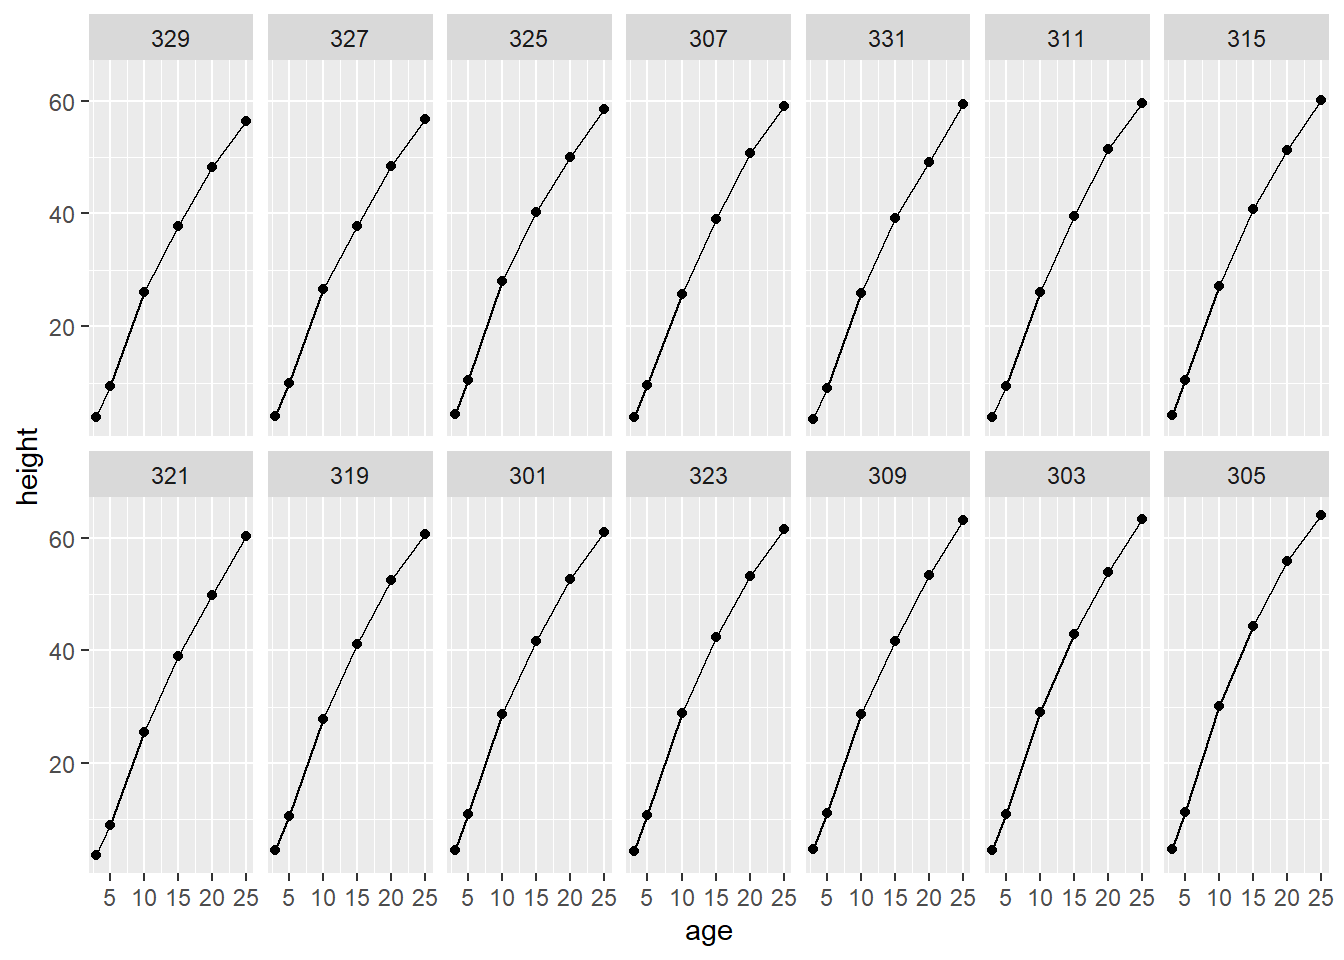
\includegraphics{GLMM_files/figure-latex/unnamed-chunk-8-1.pdf}

To model the mean height behavior we might choose a, say, third degree polynomial function of age. There are a few ways of doing this: specify a polynomial in age, a polynomial in \{age - mean(age)\}, or a basis of orthogonal polynomials. Both the second and third strategies are better than the first as coefficients of polynomial elements will be correlated unless those polynomial elements are orthogonal or the variable is centered.

It would not be appropriate to model the heights as a polynomial function of age with only those fixed effects. Since heights are recorded at the same ages for several trees, those height measurements are correlated within trees. We can capture such correlation within trees by including random, tree-specific polynomial coefficients. This polynomial mixed effects model looks like the following
\begin{align*}
Y_{ij} &= \beta_0 + \beta_1 X_{ij1}+ \beta_2 X_{ij2}+ \beta_3 X_{ij3}\\
       &+ \beta_{i1} X_{ij1}+ \beta_{i2} X_{ij2}+ \beta_{i3} X_{ij3}\\
       & + \epsilon_{ij}
\end{align*}
where \(i=1, \ldots, 14\) indexes trees, \(j = 1, \ldots, 6\) indexes ages, \(\beta_1\) through \(\beta_3\) are common coefficients for fixed polynomial age effects, and \(\beta_{i1}\) through \(\beta_{i3}\) are varying coefficients for age effects for each tree. The covariates \(X_{ij1}\) through \(X_{ij3}\) represent third degree orthogonal polynomials; i.e., they are not simply age, age\(^2\) and age\(^3\), more on those shortly. The random effects are normal with covariance \(\psi\), i.e., \((\beta_{i1},\beta_{i2},\beta_{i3})^\top \stackrel{iid}{\sim}N(0,\psi)\). The random-sampling errors are modeled as zero-mean, time-dependent normal random variables for a lag of 1, so that \((\epsilon_{i1},\ldots, \epsilon_{i6})\stackrel{iid}{\sim} N(0,\Lambda)\) where \(\Lambda\) is positive definite and tri-diagonal.

\hypertarget{model-fitting-for-loblolly-pines-data}{%
\subsection{Model-fitting for Loblolly pines data}\label{model-fitting-for-loblolly-pines-data}}

Below we specify this model using the lme function from the nlme package. With default optimization specifications lme fails to fit this model, but lme converges if we simply increase the maximum number of iterations and function evaluations via the lmeControl function.

\begin{Shaded}
\begin{Highlighting}[]
\NormalTok{lmc }\OtherTok{\textless{}{-}} \FunctionTok{lmeControl}\NormalTok{(}\AttributeTok{niterEM=}\DecValTok{1000}\NormalTok{,}\AttributeTok{msMaxIter=}\DecValTok{1000}\NormalTok{,}\AttributeTok{msMaxEval=}\DecValTok{1000}\NormalTok{)}

\NormalTok{model1 }\OtherTok{\textless{}{-}} \FunctionTok{lme}\NormalTok{(height }\SpecialCharTok{\textasciitilde{}} \FunctionTok{poly}\NormalTok{(age,}\DecValTok{3}\NormalTok{), }\AttributeTok{data =}\NormalTok{ Loblolly,}
\AttributeTok{random =} \FunctionTok{list}\NormalTok{(}\AttributeTok{Seed =} \SpecialCharTok{\textasciitilde{}} \FunctionTok{poly}\NormalTok{(age,}\DecValTok{3}\NormalTok{)),}
\AttributeTok{correlation =} \FunctionTok{corAR1}\NormalTok{(}\AttributeTok{form =} \SpecialCharTok{\textasciitilde{}}\NormalTok{ age}\SpecialCharTok{|}\NormalTok{Seed), }\AttributeTok{control =}\NormalTok{ lmc)}

\FunctionTok{summary}\NormalTok{(model1)}
\end{Highlighting}
\end{Shaded}

\begin{verbatim}
## Linear mixed-effects model fit by REML
##   Data: Loblolly 
##        AIC      BIC    logLik
##   242.2632 280.3756 -105.1316
## 
## Random effects:
##  Formula: ~poly(age, 3) | Seed
##  Structure: General positive-definite, Log-Cholesky parametrization
##               StdDev    Corr                
## (Intercept)   1.4302075 (Intr) p(,3)1 p(,3)2
## poly(age, 3)1 6.5811089  0.915              
## poly(age, 3)2 2.6961875 -0.812 -0.509       
## poly(age, 3)3 0.5943500 -0.125 -0.514 -0.477
## Residual      0.5906168                     
## 
## Correlation Structure: ARMA(1,0)
##  Formula: ~age | Seed 
##  Parameter estimate(s):
##          Phi1 
## -2.944641e-07 
## Fixed effects:  height ~ poly(age, 3) 
##                   Value Std.Error DF   t-value p-value
## (Intercept)    32.36440 0.3876331 67  83.49237   0.000
## poly(age, 3)1 186.44570 1.8553896 67 100.48870   0.000
## poly(age, 3)2 -21.84656 0.9317043 67 -23.44796   0.000
## poly(age, 3)3   0.05782 0.6116048 67   0.09454   0.925
##  Correlation: 
##               (Intr) p(,3)1 p(,3)2
## poly(age, 3)1  0.856              
## poly(age, 3)2 -0.619 -0.373       
## poly(age, 3)3 -0.032 -0.126 -0.096
## 
## Standardized Within-Group Residuals:
##         Min          Q1         Med          Q3         Max 
## -1.84043424 -0.43798962 -0.03581482  0.69326329  1.56774981 
## 
## Number of Observations: 84
## Number of Groups: 14
\end{verbatim}

While the summary function contains everything needed to determine if fixed effects are significant, it does not provide a straightforward explanation of all parameter estimates. With a little work, we can reproduce the estimated covariance parameters, and the estimated covariance of fixed effects. The getVarCov function provides the estimated covariance of the random effects nested within Seed; we could call these \(\hat\psi_i\) for seeds \(i=1, \ldots, 14\). The matrix \(\psi\) is block-diagonal, with identical blocks \(\psi_i\). The estimated residual variance is tri-diagonal with constant main diagonal elements \(\hat\sigma^2\) given by \texttt{summary(model1)\$sigma\^{}2} and constant off-diagonal elements given by \texttt{coef(model1\$modelStruct\$corStruct,\ unconstrained\ =\ FALSE)}.

The following helper function from the Matrix package can help in constructing the \(\Psi\) matrix:

\begin{Shaded}
\begin{Highlighting}[]
\NormalTok{bdiag\_m }\OtherTok{\textless{}{-}} \ControlFlowTok{function}\NormalTok{(lmat) \{}
    \DocumentationTok{\#\# Copyright (C) 2016 Martin Maechler, ETH Zurich}
    \ControlFlowTok{if}\NormalTok{(}\SpecialCharTok{!}\FunctionTok{length}\NormalTok{(lmat)) }\FunctionTok{return}\NormalTok{(}\FunctionTok{new}\NormalTok{(}\StringTok{"dgCMatrix"}\NormalTok{))}
    \FunctionTok{stopifnot}\NormalTok{(}\FunctionTok{is.list}\NormalTok{(lmat), }\FunctionTok{is.matrix}\NormalTok{(lmat[[}\DecValTok{1}\NormalTok{]]),}
\NormalTok{              (k }\OtherTok{\textless{}{-}}\NormalTok{ (d }\OtherTok{\textless{}{-}} \FunctionTok{dim}\NormalTok{(lmat[[}\DecValTok{1}\NormalTok{]]))[}\DecValTok{1}\NormalTok{]) }\SpecialCharTok{==}\NormalTok{ d[}\DecValTok{2}\NormalTok{], }\CommentTok{\# k x k}
              \FunctionTok{all}\NormalTok{(}\FunctionTok{vapply}\NormalTok{(lmat, dim, }\FunctionTok{integer}\NormalTok{(}\DecValTok{2}\NormalTok{)) }\SpecialCharTok{==}\NormalTok{ k)) }\CommentTok{\# all of them}
\NormalTok{    N }\OtherTok{\textless{}{-}} \FunctionTok{length}\NormalTok{(lmat)}
    \ControlFlowTok{if}\NormalTok{(N }\SpecialCharTok{*}\NormalTok{ k }\SpecialCharTok{\textgreater{}}\NormalTok{ .Machine}\SpecialCharTok{$}\NormalTok{integer.max)}
        \FunctionTok{stop}\NormalTok{(}\StringTok{"resulting matrix too large; would be  M x M, with M="}\NormalTok{, N}\SpecialCharTok{*}\NormalTok{k)}
\NormalTok{    M }\OtherTok{\textless{}{-}} \FunctionTok{as.integer}\NormalTok{(N }\SpecialCharTok{*}\NormalTok{ k)}
    \DocumentationTok{\#\# result: an   M x M  matrix}
    \FunctionTok{new}\NormalTok{(}\StringTok{"dgCMatrix"}\NormalTok{, }\AttributeTok{Dim =} \FunctionTok{c}\NormalTok{(M,M),}
        \DocumentationTok{\#\# \textquotesingle{}i :\textquotesingle{} maybe there\textquotesingle{}s a faster way (w/o matrix indexing), but elegant?}
        \AttributeTok{i =} \FunctionTok{as.vector}\NormalTok{(}\FunctionTok{matrix}\NormalTok{(0L}\SpecialCharTok{:}\NormalTok{(M}\SpecialCharTok{{-}}\NormalTok{1L), }\AttributeTok{nrow=}\NormalTok{k)[, }\FunctionTok{rep}\NormalTok{(}\FunctionTok{seq\_len}\NormalTok{(N), }\AttributeTok{each=}\NormalTok{k)]),}
        \AttributeTok{p =}\NormalTok{ k }\SpecialCharTok{*}\NormalTok{ 0L}\SpecialCharTok{:}\NormalTok{M,}
        \AttributeTok{x =} \FunctionTok{as.double}\NormalTok{(}\FunctionTok{unlist}\NormalTok{(lmat, }\AttributeTok{recursive=}\ConstantTok{FALSE}\NormalTok{, }\AttributeTok{use.names=}\ConstantTok{FALSE}\NormalTok{)))}
\NormalTok{\}}
\end{Highlighting}
\end{Shaded}

We can match the standard errors and approximate p-values of the fixed effects using the following calculations (more on p-values later). One thing to mention: the \(Z\) design matrix of random effects seems not present in the lme object, and so we fit the same type of model using lmer from the lme4 package that more easily allows us to obtain this model matrix.

\begin{Shaded}
\begin{Highlighting}[]
\FunctionTok{library}\NormalTok{(lme4)}
\end{Highlighting}
\end{Shaded}

\begin{verbatim}
## Loading required package: Matrix
\end{verbatim}

\begin{verbatim}
## 
## Attaching package: 'lme4'
\end{verbatim}

\begin{verbatim}
## The following object is masked from 'package:nlme':
## 
##     lmList
\end{verbatim}

\begin{Shaded}
\begin{Highlighting}[]
\NormalTok{model2lmer }\OtherTok{\textless{}{-}} \FunctionTok{lmer}\NormalTok{(height }\SpecialCharTok{\textasciitilde{}} \FunctionTok{poly}\NormalTok{(age,}\DecValTok{3}\NormalTok{) }\SpecialCharTok{+}\NormalTok{ (}\FunctionTok{poly}\NormalTok{(age,}\DecValTok{3}\NormalTok{) }\SpecialCharTok{|}\NormalTok{ Seed), }\AttributeTok{data =}\NormalTok{ Loblolly, }\AttributeTok{control =} \FunctionTok{lmerControl}\NormalTok{(}\AttributeTok{optimizer=}\StringTok{"Nelder\_Mead"}\NormalTok{, }\AttributeTok{optCtrl =} \FunctionTok{list}\NormalTok{(}\AttributeTok{maxfun =} \DecValTok{100000}\NormalTok{), }\AttributeTok{check.conv.grad =} \FunctionTok{.makeCC}\NormalTok{(}\StringTok{"warning"}\NormalTok{, }\AttributeTok{tol =} \FloatTok{0.71}\NormalTok{, }\AttributeTok{relTol =} \ConstantTok{NULL}\NormalTok{)))}
\NormalTok{Z }\OtherTok{\textless{}{-}} \FunctionTok{model.matrix}\NormalTok{(model2lmer, }\AttributeTok{type =} \StringTok{\textquotesingle{}random\textquotesingle{}}\NormalTok{)}
\NormalTok{psi\_i }\OtherTok{\textless{}{-}} \FunctionTok{getVarCov}\NormalTok{(model1)}
\NormalTok{psi }\OtherTok{\textless{}{-}} \FunctionTok{bdiag\_m}\NormalTok{(}\FunctionTok{list}\NormalTok{(psi\_i,psi\_i,psi\_i,psi\_i,psi\_i,psi\_i,psi\_i,psi\_i,psi\_i,psi\_i,psi\_i,psi\_i,psi\_i,psi\_i))}
\NormalTok{inv\_psi }\OtherTok{\textless{}{-}} \FunctionTok{solve}\NormalTok{(psi)}
\NormalTok{phi }\OtherTok{\textless{}{-}} \FunctionTok{coef}\NormalTok{(model1}\SpecialCharTok{$}\NormalTok{modelStruct}\SpecialCharTok{$}\NormalTok{corStruct, }\AttributeTok{unconstrained =} \ConstantTok{FALSE}\NormalTok{)}
\NormalTok{L }\OtherTok{\textless{}{-}}\NormalTok{ (}\FunctionTok{summary}\NormalTok{(model1)}\SpecialCharTok{$}\NormalTok{sigma}\SpecialCharTok{\^{}}\DecValTok{2}\NormalTok{)}\SpecialCharTok{*}\FunctionTok{diag}\NormalTok{(}\FunctionTok{nrow}\NormalTok{(Loblolly))}
\ControlFlowTok{for}\NormalTok{(i }\ControlFlowTok{in} \DecValTok{1}\SpecialCharTok{:}\FunctionTok{nrow}\NormalTok{(L))\{}
  \ControlFlowTok{for}\NormalTok{(j }\ControlFlowTok{in} \FunctionTok{nrow}\NormalTok{(L))\{}
    \ControlFlowTok{if}\NormalTok{(j}\SpecialCharTok{==}\NormalTok{(i}\SpecialCharTok{+}\DecValTok{1}\NormalTok{)}\SpecialCharTok{||}\NormalTok{j}\SpecialCharTok{==}\NormalTok{(i}\DecValTok{{-}1}\NormalTok{))\{}
\NormalTok{      L[i,j] }\OtherTok{\textless{}{-}}\NormalTok{ phi}
\NormalTok{    \}}
\NormalTok{  \}}
\NormalTok{\}}
\NormalTok{invL }\OtherTok{\textless{}{-}} \FunctionTok{solve}\NormalTok{(L)}
\NormalTok{A }\OtherTok{\textless{}{-}}\NormalTok{ inv\_psi}\SpecialCharTok{+}\FunctionTok{t}\NormalTok{(Z)}\SpecialCharTok{\%*\%}\NormalTok{invL}\SpecialCharTok{\%*\%}\NormalTok{Z}
\NormalTok{invA }\OtherTok{\textless{}{-}} \FunctionTok{solve}\NormalTok{(A)}
\NormalTok{P}\OtherTok{\textless{}{-}}\NormalTok{invL}\SpecialCharTok{{-}}\NormalTok{invL}\SpecialCharTok{\%*\%}\NormalTok{Z}\SpecialCharTok{\%*\%}\NormalTok{invA}\SpecialCharTok{\%*\%}\FunctionTok{t}\NormalTok{(Z)}\SpecialCharTok{\%*\%}\NormalTok{invL}
\NormalTok{X }\OtherTok{\textless{}{-}} \FunctionTok{model.matrix}\NormalTok{(model2lmer, }\AttributeTok{type =} \StringTok{\textquotesingle{}fixed\textquotesingle{}}\NormalTok{)}
\NormalTok{cov.beta.hat }\OtherTok{\textless{}{-}} \FunctionTok{solve}\NormalTok{(}\FunctionTok{t}\NormalTok{(X)}\SpecialCharTok{\%*\%}\NormalTok{P}\SpecialCharTok{\%*\%}\NormalTok{X)}
\NormalTok{Y }\OtherTok{\textless{}{-}}\NormalTok{ Loblolly}\SpecialCharTok{$}\NormalTok{height}
\NormalTok{beta.hat }\OtherTok{\textless{}{-}}\NormalTok{ cov.beta.hat}\SpecialCharTok{\%*\%}\FunctionTok{t}\NormalTok{(X)}\SpecialCharTok{\%*\%}\NormalTok{P}\SpecialCharTok{\%*\%}\NormalTok{Y}
\NormalTok{beta.hat}
\end{Highlighting}
\end{Shaded}

\begin{verbatim}
## 4 x 1 Matrix of class "dgeMatrix"
##              [,1]
## [1,]  32.36440477
## [2,] 186.44569514
## [3,] -21.84656380
## [4,]   0.05781863
\end{verbatim}

\begin{Shaded}
\begin{Highlighting}[]
\NormalTok{cov.beta.hat}
\end{Highlighting}
\end{Shaded}

\begin{verbatim}
## 4 x 4 Matrix of class "dgeMatrix"
##              [,1]       [,2]        [,3]         [,4]
## [1,]  0.150259390  0.6154960 -0.22367703 -0.007593674
## [2,]  0.615495986  3.4424706 -0.64470993 -0.143514475
## [3,] -0.223677034 -0.6447099  0.86807296 -0.054643528
## [4,] -0.007593673 -0.1435145 -0.05464352  0.374060450
\end{verbatim}

\begin{Shaded}
\begin{Highlighting}[]
\NormalTok{beta.hat }\SpecialCharTok{/} \FunctionTok{sqrt}\NormalTok{(}\FunctionTok{diag}\NormalTok{(cov.beta.hat)) }\CommentTok{\# t{-}values}
\end{Highlighting}
\end{Shaded}

\begin{verbatim}
## 4 x 1 Matrix of class "dgeMatrix"
##              [,1]
## [1,]  83.49237468
## [2,] 100.48870309
## [3,] -23.44795779
## [4,]   0.09453594
\end{verbatim}

\begin{Shaded}
\begin{Highlighting}[]
\DecValTok{1}\SpecialCharTok{{-}}\FunctionTok{pchisq}\NormalTok{(}\FunctionTok{as.numeric}\NormalTok{((beta.hat }\SpecialCharTok{/} \FunctionTok{sqrt}\NormalTok{(}\FunctionTok{diag}\NormalTok{(cov.beta.hat)))}\SpecialCharTok{\^{}}\DecValTok{2}\NormalTok{), }\DecValTok{1}\NormalTok{) }\CommentTok{\# rough p{-}values}
\end{Highlighting}
\end{Shaded}

\begin{verbatim}
## [1] 0.0000000 0.0000000 0.0000000 0.9246834
\end{verbatim}

\begin{Shaded}
\begin{Highlighting}[]
\DecValTok{1}\SpecialCharTok{{-}}\FunctionTok{pf}\NormalTok{(}\FunctionTok{as.numeric}\NormalTok{((beta.hat }\SpecialCharTok{/} \FunctionTok{sqrt}\NormalTok{(}\FunctionTok{diag}\NormalTok{(cov.beta.hat)))}\SpecialCharTok{\^{}}\DecValTok{2}\NormalTok{), }\DecValTok{1}\NormalTok{, }\FunctionTok{nrow}\NormalTok{(Loblolly)}\SpecialCharTok{{-}}\DecValTok{4}\NormalTok{)}
\end{Highlighting}
\end{Shaded}

\begin{verbatim}
## [1] 0.0000000 0.0000000 0.0000000 0.9249198
\end{verbatim}

You may have noticed the estimated auto-regressive covariance term is essentially zero. This motivates us to fit a nested model in which this covariance term is zero, i.e., the residual covariance structure of \(\epsilon_i\), \(i=1, \ldots, n\) is simply iid with variance \(\sigma^2\).

\begin{Shaded}
\begin{Highlighting}[]
\NormalTok{model2 }\OtherTok{\textless{}{-}} \FunctionTok{lme}\NormalTok{(height }\SpecialCharTok{\textasciitilde{}} \FunctionTok{poly}\NormalTok{(age,}\DecValTok{3}\NormalTok{), }\AttributeTok{data =}\NormalTok{ Loblolly,}
\AttributeTok{random =} \FunctionTok{list}\NormalTok{(}\AttributeTok{Seed =} \SpecialCharTok{\textasciitilde{}} \FunctionTok{poly}\NormalTok{(age,}\DecValTok{3}\NormalTok{)),}
\AttributeTok{correlation =} \ConstantTok{NULL}\NormalTok{, }\AttributeTok{control =}\NormalTok{ lmc)}

\FunctionTok{summary}\NormalTok{(model2)}
\end{Highlighting}
\end{Shaded}

\begin{verbatim}
## Linear mixed-effects model fit by REML
##   Data: Loblolly 
##        AIC      BIC    logLik
##   240.2632 275.9936 -105.1316
## 
## Random effects:
##  Formula: ~poly(age, 3) | Seed
##  Structure: General positive-definite, Log-Cholesky parametrization
##               StdDev    Corr                
## (Intercept)   1.4301995 (Intr) p(,3)1 p(,3)2
## poly(age, 3)1 6.5810089  0.915              
## poly(age, 3)2 2.6961948 -0.812 -0.509       
## poly(age, 3)3 0.5943572 -0.125 -0.514 -0.477
## Residual      0.5906184                     
## 
## Fixed effects:  height ~ poly(age, 3) 
##                   Value Std.Error DF   t-value p-value
## (Intercept)    32.36440 0.3876310 67  83.49282   0.000
## poly(age, 3)1 186.44570 1.8553648 67 100.49005   0.000
## poly(age, 3)2 -21.84656 0.9317069 67 -23.44789   0.000
## poly(age, 3)3   0.05782 0.6116069 67   0.09454   0.925
##  Correlation: 
##               (Intr) p(,3)1 p(,3)2
## poly(age, 3)1  0.856              
## poly(age, 3)2 -0.619 -0.373       
## poly(age, 3)3 -0.032 -0.126 -0.096
## 
## Standardized Within-Group Residuals:
##         Min          Q1         Med          Q3         Max 
## -1.84042613 -0.43799912 -0.03581492  0.69325898  1.56775714 
## 
## Number of Observations: 84
## Number of Groups: 14
\end{verbatim}

NLME is not the only package for fitting linear mixed models. LME4 is a newer package compared to NLME, and generally fits models much faster thanks to its better use of efficient linear algebra routines. However, LME4 is not as flexible as NLME when it comes to the available residual covariance structures one is able to fit. For example, LME4 does not have the flexibility to fit the AR(1) structure we fit for model1 above using the NLME package.

Below we fit model2 using lme4. The lmer model fitting function fails to fit the model with the default settings, much like the lme function from the nlme package. The main issue causing lack of convergence is a check function that evaluates the gradient of the likelihood at the final parameter estimates and requires it to be near zero. We have to violate this criteria in order to get the model to fit, which we can do by using the \texttt{check.conv.grad} argument of the control argument. Once we coerce lmer to converge using these options we see that it produces essentially the same estimates as lme with respect to model2.

\begin{Shaded}
\begin{Highlighting}[]
\FunctionTok{library}\NormalTok{(lme4)}
\NormalTok{model2lmer }\OtherTok{\textless{}{-}} \FunctionTok{lmer}\NormalTok{(height }\SpecialCharTok{\textasciitilde{}} \FunctionTok{poly}\NormalTok{(age,}\DecValTok{3}\NormalTok{) }\SpecialCharTok{+}\NormalTok{ (}\FunctionTok{poly}\NormalTok{(age,}\DecValTok{3}\NormalTok{) }\SpecialCharTok{|}\NormalTok{ Seed), }\AttributeTok{data =}\NormalTok{ Loblolly, }\AttributeTok{control =} \FunctionTok{lmerControl}\NormalTok{(}\AttributeTok{optimizer=}\StringTok{"Nelder\_Mead"}\NormalTok{, }\AttributeTok{optCtrl =} \FunctionTok{list}\NormalTok{(}\AttributeTok{maxfun =} \DecValTok{100000}\NormalTok{), }\AttributeTok{check.conv.grad =} \FunctionTok{.makeCC}\NormalTok{(}\StringTok{"warning"}\NormalTok{, }\AttributeTok{tol =} \FloatTok{0.71}\NormalTok{, }\AttributeTok{relTol =} \ConstantTok{NULL}\NormalTok{)))}
\FunctionTok{summary}\NormalTok{(model2lmer)}
\end{Highlighting}
\end{Shaded}

\begin{verbatim}
## Linear mixed model fit by REML ['lmerMod']
## Formula: height ~ poly(age, 3) + (poly(age, 3) | Seed)
##    Data: Loblolly
## Control: 
## lmerControl(optimizer = "Nelder_Mead", optCtrl = list(maxfun = 1e+05),  
##     check.conv.grad = .makeCC("warning", tol = 0.71, relTol = NULL))
## 
## REML criterion at convergence: 210.6
## 
## Scaled residuals: 
##      Min       1Q   Median       3Q      Max 
## -1.83857 -0.45408 -0.02587  0.65608  1.54812 
## 
## Random effects:
##  Groups   Name          Variance Std.Dev. Corr             
##  Seed     (Intercept)    1.9497  1.3963                    
##           poly(age, 3)1 40.8246  6.3894    0.91            
##           poly(age, 3)2  7.2430  2.6913   -0.82 -0.50      
##           poly(age, 3)3  0.6555  0.8096   -0.03 -0.37 -0.44
##  Residual                0.3506  0.5922                    
## Number of obs: 84, groups:  Seed, 14
## 
## Fixed effects:
##                Estimate Std. Error t value
## (Intercept)    32.36440    0.37873  85.455
## poly(age, 3)1 186.44570    1.80740 103.157
## poly(age, 3)2 -21.84656    0.93167 -23.449
## poly(age, 3)3   0.05782    0.63045   0.092
## 
## Correlation of Fixed Effects:
##             (Intr) p(,3)1 p(,3)2
## poly(ag,3)1  0.846              
## poly(ag,3)2 -0.621 -0.367       
## poly(ag,3)3 -0.011 -0.119 -0.117
\end{verbatim}

Next, we will investigate various residual quantities to determine if our model assumptions are plausible.

\hypertarget{model-diagnostics}{%
\section{Model diagnostics}\label{model-diagnostics}}

As in pure fixed effects linear models, residuals are helpful for checking assumptions like linearity and normality. For mixed effects models, there are more ways to define residuals:
- Marginal residuals are the residuals formed by subtracting the fitted fixed effect from the response, that is, \(\hat e_{ij} := Y_{ij} - x_{ij}^\top \hat\beta\)
- Standardized marginal residuals remove the effect of correlation within groups. Let \(\hat\Sigma_i\) denote the fitted covariance within group \(i\), and let \(\hat\Sigma_i^{-1/2}\) denote the lower Cholesky factor of \(\hat\Sigma_i^{-1}\). Then, \(\hat \epsilon_{i} = \hat\Sigma_i^{-1/2}\hat e_i\) denotes the vector of standardized marginal residuals for group \(i\).
- Conditional residuals also subtract the predicted random effect, \(\hat \xi_{ij} = Y_{ij} - x_{ij}^\top \hat\beta - z_{ij}^\top \hat \alpha\)
- Standardized conditional residuals \(\hat\phi_{ij}\) are formed by standardizing the conditional residuals by \(\hat\sigma\sqrt{v_{kk}}\) where \(\hat\sigma\) is the fitted residual standard error and \(v_{kk}\) is the \(k^{th}\) diagonal entry of the matrix \(I_n - X(X^\top \hat \Sigma^{-1} X)^{-1}X^\top\).

A scatterplot of marginal residuals versus fixed covariates are useful for checking the assumption of linearity. Trends in this plot indicate an important omitted variable and/or nonlinearity.

Quantile-quantile plots of standardized marginal residuals should match a standard normal distribution. If not, then the chosen covariance structure is not good model for the given data. comparing quantile-quantile plots for each group can be useful for assessing heteroskedasticity, although these comparisons become rough when groups have few individuals.

Large absolute standardized conditional residuals are indicate outliers. Plots of standardized conditional residuals versus the fitted values \(X\hat\beta + Z\hat\alpha\) may also reveal heteroskedasticity at the individual level---which would suggest modifying the structure of \(\Lambda\) if it is assumed to be \(\sigma^2 I_n\) as is common.

Both conditional and standardized conditional residuals are confounded with the best linear unbiased predictors \(Z\hat\alpha\) in the sense they depend on each other. The degree of this confounding interferes with the standardized conditional residuals ability to indicate normality (or lack of normality) of the conditional errors. A correction, termed the least confounded residuals, aims to construct a residual better able to detect departures from normality. The correction is performed by way of solving a generalized eigenvalue problem. Let matrices \(A\) and \(B\) denote \(A = (I_n - X(X^\top \hat \Sigma^{-1} X)^{-1}X^\top)\hat\Sigma^{-1}I_n - X(X^\top \hat \Sigma^{-1} X)^{-1}X^\top\) and \(B = I_n - X(X^\top \hat \Sigma^{-1} X)^{-1}X^\top\). The least confounded residuals are \(t^\top \hat\phi_{ij}\) where \(t\) maximizes \((t^\top A t) / (t^\top B t)\). The maximum value occurs at the largest eigenvalue of \(B^{-1}A\) and \(t\) is the corresponding eigenvector.

\hypertarget{model-diagnostics-for-loblolly-pines-data}{%
\subsection{Model diagnostics for Loblolly pines data}\label{model-diagnostics-for-loblolly-pines-data}}

\begin{Shaded}
\begin{Highlighting}[]
\NormalTok{Loblolly}\SpecialCharTok{$}\NormalTok{fitted3 }\OtherTok{\textless{}{-}} \FunctionTok{fitted}\NormalTok{(model2lmer)}

\FunctionTok{ggplot}\NormalTok{(}\AttributeTok{data =}\NormalTok{ Loblolly) }\SpecialCharTok{+} 
  \FunctionTok{geom\_line}\NormalTok{(}\AttributeTok{mapping =} \FunctionTok{aes}\NormalTok{(}\AttributeTok{x =}\NormalTok{ age, }\AttributeTok{y =}\NormalTok{ height)) }\SpecialCharTok{+} 
  \FunctionTok{geom\_point}\NormalTok{(}\AttributeTok{mapping =} \FunctionTok{aes}\NormalTok{(}\AttributeTok{x =}\NormalTok{ age, }\AttributeTok{y =}\NormalTok{ height)) }\SpecialCharTok{+} 
  \FunctionTok{geom\_point}\NormalTok{(}\AttributeTok{mapping =} \FunctionTok{aes}\NormalTok{(}\AttributeTok{x =}\NormalTok{ age, }\AttributeTok{y =}\NormalTok{ fitted3, }\AttributeTok{color =} \StringTok{\textquotesingle{}red\textquotesingle{}}\NormalTok{)) }\SpecialCharTok{+}
  \FunctionTok{facet\_wrap}\NormalTok{(}\SpecialCharTok{\textasciitilde{}}\NormalTok{ Seed, }\AttributeTok{nrow =} \DecValTok{2}\NormalTok{)}
\end{Highlighting}
\end{Shaded}

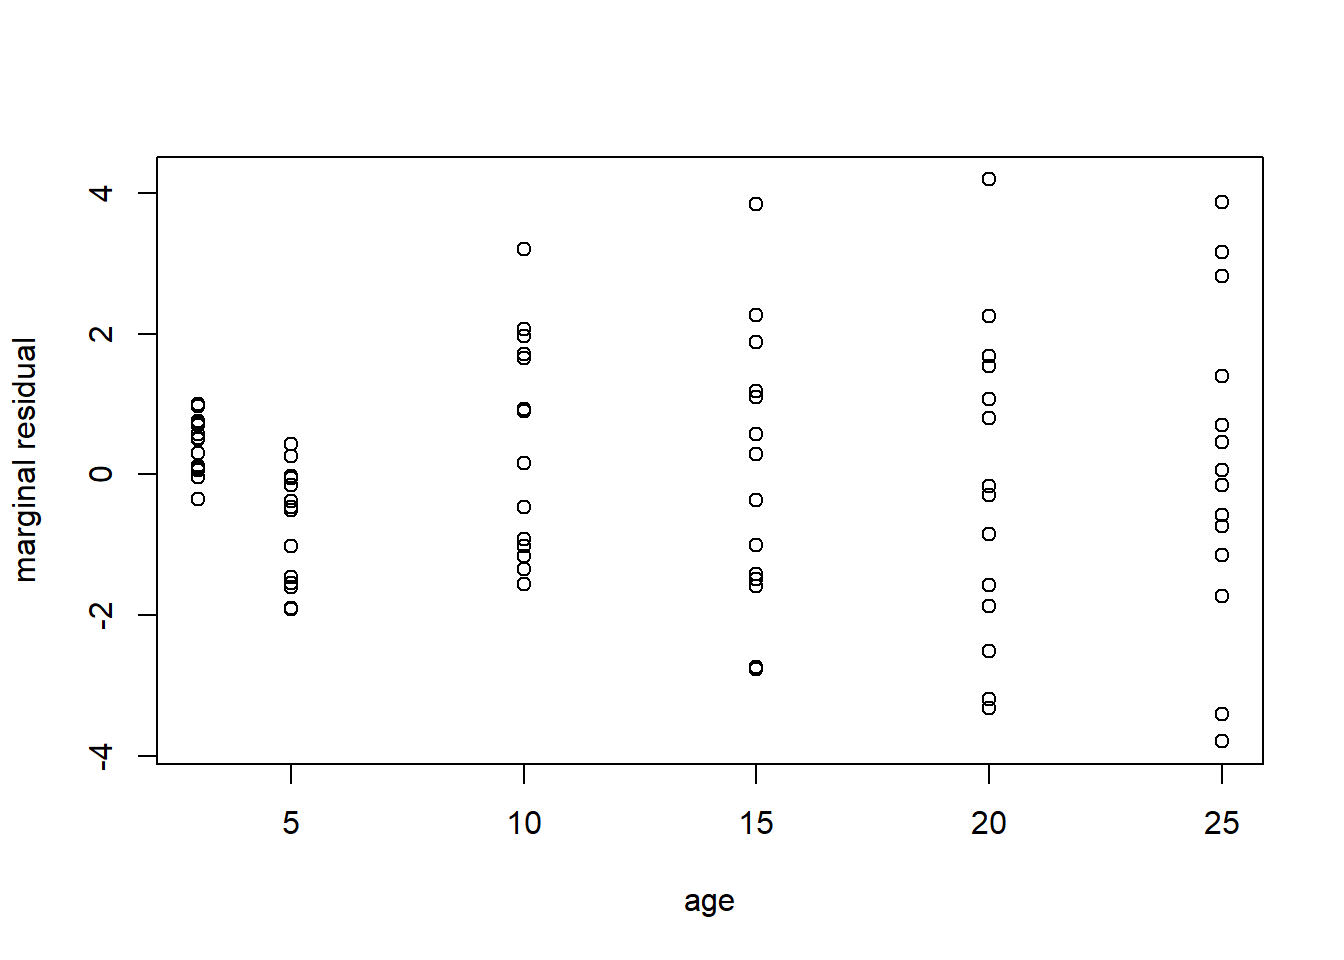
\includegraphics{GLMM_files/figure-latex/unnamed-chunk-14-1.pdf}

\begin{Shaded}
\begin{Highlighting}[]
\NormalTok{marginal.resids }\OtherTok{\textless{}{-}}\NormalTok{ Loblolly}\SpecialCharTok{$}\NormalTok{height }\SpecialCharTok{{-}} \FunctionTok{model.matrix}\NormalTok{(model2lmer, }\AttributeTok{type =} \StringTok{\textquotesingle{}fixed\textquotesingle{}}\NormalTok{)}\SpecialCharTok{\%*\%}\FunctionTok{fixef}\NormalTok{(model2lmer)}

\FunctionTok{plot}\NormalTok{(Loblolly}\SpecialCharTok{$}\NormalTok{age, marginal.resids, }\AttributeTok{xlab =} \StringTok{\textquotesingle{}age\textquotesingle{}}\NormalTok{, }\AttributeTok{ylab =} \StringTok{\textquotesingle{}marginal residual\textquotesingle{}}\NormalTok{)}
\end{Highlighting}
\end{Shaded}

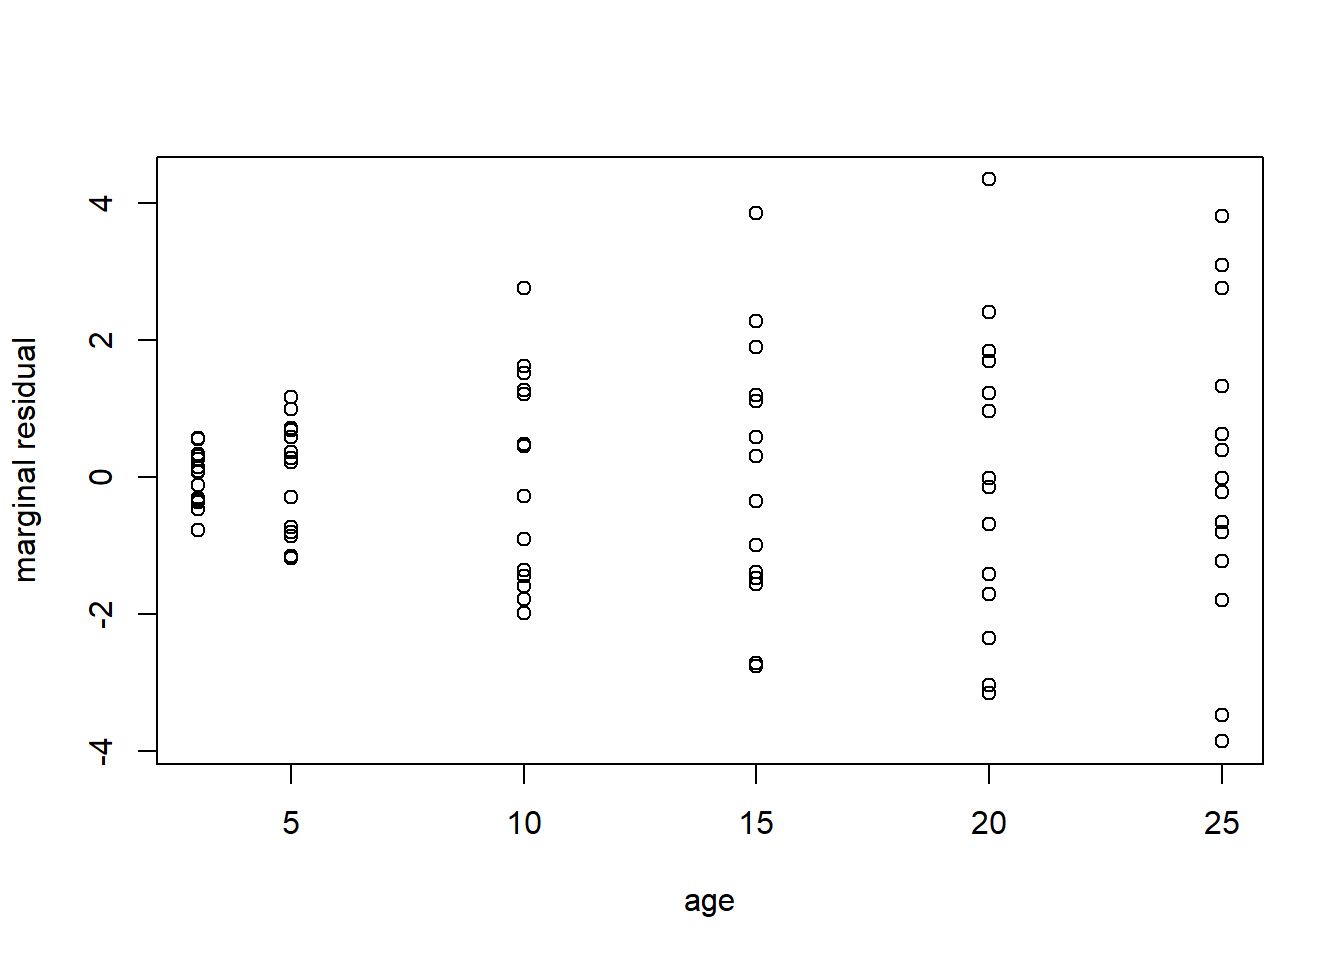
\includegraphics{GLMM_files/figure-latex/unnamed-chunk-15-1.pdf}

\begin{Shaded}
\begin{Highlighting}[]
\FunctionTok{plot}\NormalTok{(Loblolly}\SpecialCharTok{$}\NormalTok{Seed, marginal.resids, }\AttributeTok{xlab =} \StringTok{\textquotesingle{}Seed\textquotesingle{}}\NormalTok{, }\AttributeTok{ylab =} \StringTok{\textquotesingle{}marginal residual\textquotesingle{}}\NormalTok{)}
\end{Highlighting}
\end{Shaded}

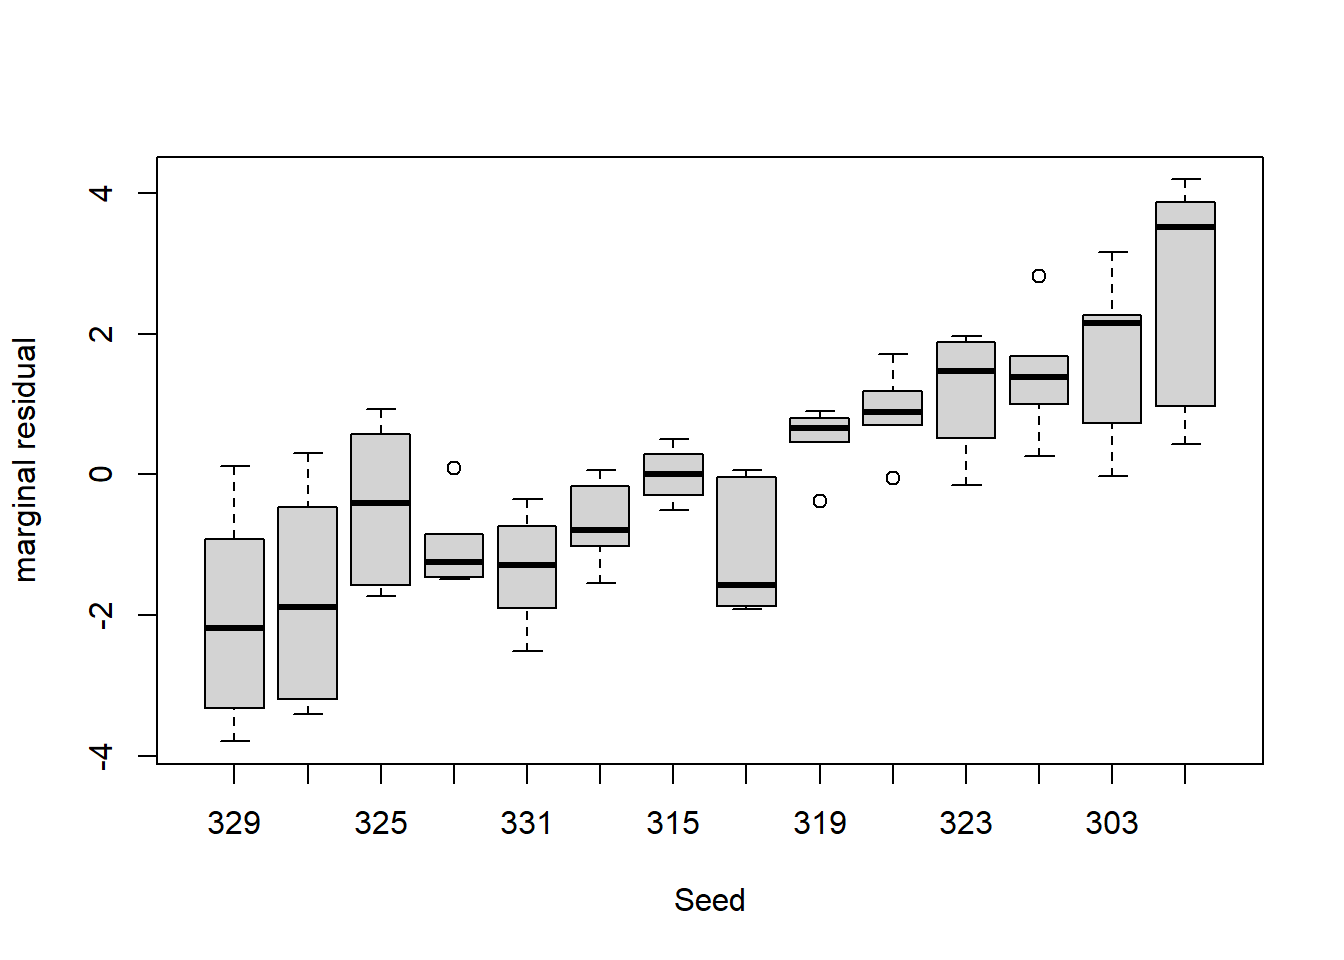
\includegraphics{GLMM_files/figure-latex/unnamed-chunk-15-2.pdf}

\begin{Shaded}
\begin{Highlighting}[]
\NormalTok{Pi }\OtherTok{\textless{}{-}} \FunctionTok{as.matrix}\NormalTok{(P)[}\DecValTok{1}\SpecialCharTok{:}\DecValTok{6}\NormalTok{,}\DecValTok{1}\SpecialCharTok{:}\DecValTok{6}\NormalTok{]}
\NormalTok{cholPi }\OtherTok{\textless{}{-}} \FunctionTok{chol}\NormalTok{(Pi)}
\NormalTok{standardized\_resids }\OtherTok{\textless{}{-}} \FunctionTok{rep}\NormalTok{(}\ConstantTok{NA}\NormalTok{,}\DecValTok{84}\NormalTok{)}
\NormalTok{seed}\OtherTok{=}\DecValTok{1}
\ControlFlowTok{for}\NormalTok{(i }\ControlFlowTok{in} \DecValTok{1}\SpecialCharTok{:}\DecValTok{14}\NormalTok{)\{}
\NormalTok{  standardized\_resids[(seed}\DecValTok{{-}1}\NormalTok{)}\SpecialCharTok{*}\DecValTok{6}\SpecialCharTok{+}\NormalTok{(}\DecValTok{1}\SpecialCharTok{:}\DecValTok{6}\NormalTok{)] }\OtherTok{\textless{}{-}} \FunctionTok{t}\NormalTok{(cholPi)}\SpecialCharTok{\%*\%}\NormalTok{marginal.resids[(seed}\DecValTok{{-}1}\NormalTok{)}\SpecialCharTok{*}\DecValTok{6}\SpecialCharTok{+}\NormalTok{(}\DecValTok{1}\SpecialCharTok{:}\DecValTok{6}\NormalTok{)]}
\NormalTok{  seed }\OtherTok{\textless{}{-}}\NormalTok{ seed }\SpecialCharTok{+} \DecValTok{1}
\NormalTok{\}}
\FunctionTok{qqnorm}\NormalTok{(standardized\_resids)}
\FunctionTok{qqline}\NormalTok{(standardized\_resids)}
\end{Highlighting}
\end{Shaded}

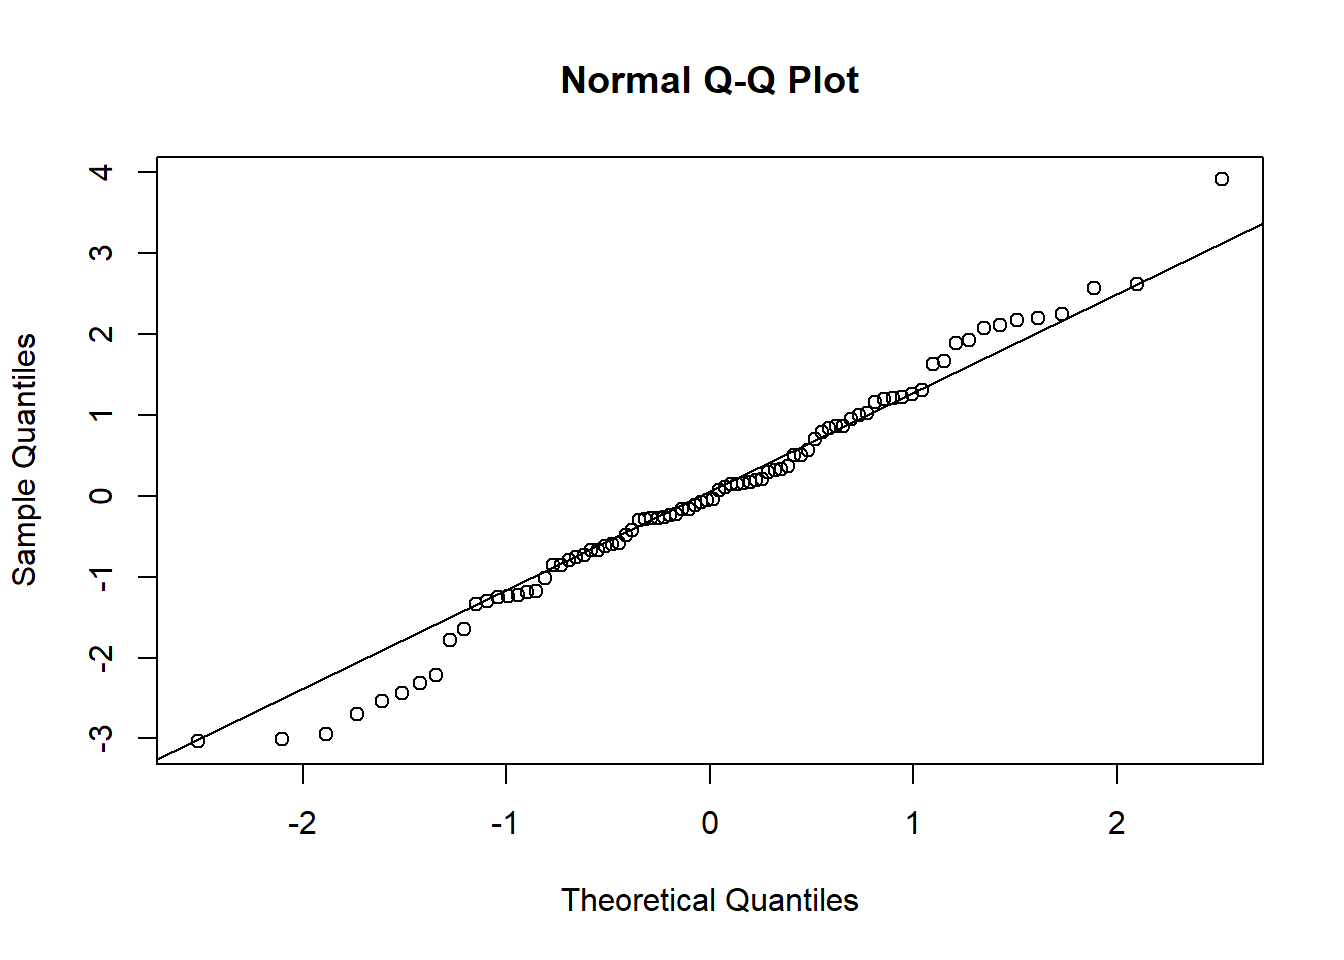
\includegraphics{GLMM_files/figure-latex/unnamed-chunk-15-3.pdf}

\begin{Shaded}
\begin{Highlighting}[]
\FunctionTok{sum}\NormalTok{((}\FunctionTok{diag}\NormalTok{(}\DecValTok{6}\NormalTok{) }\SpecialCharTok{{-}}\NormalTok{ standardized\_resids[}\DecValTok{1}\SpecialCharTok{:}\DecValTok{6}\NormalTok{]}\SpecialCharTok{\%*\%}\FunctionTok{t}\NormalTok{(standardized\_resids[}\DecValTok{1}\SpecialCharTok{:}\DecValTok{6}\NormalTok{]))}\SpecialCharTok{\^{}}\DecValTok{2}\NormalTok{)}
\end{Highlighting}
\end{Shaded}

\begin{verbatim}
## [1] 39.83443
\end{verbatim}

Next, we will discuss inference for fixed effects and model comparisons.

\hypertarget{inference-for-fixed-effects-random-effects-and-model-comparisons}{%
\section{Inference for fixed effects, random effects, and model comparisons}\label{inference-for-fixed-effects-random-effects-and-model-comparisons}}

The most common inferential questions concern the regression coefficient vector \(\beta\). Wald confidence regions for \(\beta\) are defined by the sets
\[C_\alpha := \{b: (b - \hat\beta)(X^\top V^{-1}X)^{-1}(b - \hat\beta)<\chi^2_{1-\alpha, p}\}\]
where \(\chi^2_{1-\alpha, p}\) is the upper \(\alpha\) quantile of the Chi-squared distribution with \(p\) degrees of freedom. Unfortunately, these regions are only exact when \(\theta\) is known and can severely undercover for small sample sizes. Software packages typically perform an adjustment, such as the Kenward-Rogers scaling, which is a generalization of Satterthwaite's approximation.

For a point null hypothesis \(H_0: \beta = \beta_{0}\) the Wald test statistic is
\[W = (\beta_0 - \hat\beta)(X^\top V^{-1}X)^{-1}(\beta_0 - \hat\beta)\]
and \(H_0\) is rejected if \(W > \chi^2_{1-\alpha, p}\). More generally, let \(D\) denote an \(r\times p\) matrix \(r<p\) of full rank. Reject the null hypothesis \(H_0:D\beta = b_0\) if \(W > \chi^2_{1-\alpha, r}\) where
\[W = (b_0 - D\hat\beta)(D X^\top V^{-1}X D^\top)^{-1}(b_0 - D\hat\beta)\]

(Generalized) Likelihood ratio tests may be used to compare \emph{nested} models. Model A is nested in B if A may be written as B with some of B's parameters equal to zero, provided zero is not a boundary value for the parameter being omitted in model A. For example, A is nested in B if A contains only a subset of B's fixed effects, a subset of B's random effects, a nested residual covariance structure like iid versus AR(1) as in the above example, or a combination of these three. When likelihood ratio tests are performed to compare nested models with different fixed effects both models should be fit using maximum likelihood rather than REML because residual likelihoods for two different sets of fixed effects are not comparable.

An example of models that are not nested is the cubic model above called model1 versus a model with linear, quadratic and fourth order fixed effects but no third order fixed effect. AIC and/or BIC comparisons (based on the full likelihoods) are useful for comparing non-nested models (remember: lower AIC/BIC is better).

As mentioned previously, in the context of linear mixed models, test statistics rarely have exact Chi-squared or F null distributions---the exceptions pertain to balanced experiments. In fact, these approximations may be very rough, depending on the model and sample sizes. For this reason, the LMER package does not even report p-values at this time. But, there are a few options for producing fairly reliable p-values. One option is to utilize the lmerTest package which provides functions for testing fixed effects using Satterthwaite or Kenward-Rogers corrected null distributions. Another option is to use the parametric bootstrap (based on sampling a multivariate normal distribution) to provide bootstrap-based tests and confidence intervals. The bootstrap method is endorsed by the creators of LME4, and they have included the bootMer function in that package to facilitate bootstrap-based inference in linear mixed models.

\hypertarget{inference-on-fixed-effects-for-loblolly-pines-data}{%
\subsection{Inference on fixed effects for Loblolly pines data}\label{inference-on-fixed-effects-for-loblolly-pines-data}}

The first question of interest, which we hinted at before, is whether or not we need to model the residual error as having a time-dependent, e.g., AR(1), structure. Recall our point estimate for the auto-regressive correlation was essentially zero, suggesting it played no role in the model fit. The NLME package contains an anova method for comparing models. While we should get into the habit of comparing models fit by maximum likelihood, it makes little difference if we use REML for this comparison because the models only differ in covariance structure, not fixed-effects structure. Whether we compare models fit by REML or ML, we see overwhelming evidence that the simpler model, the one without an auto-regressive error structure, is just as good as the more complicated model.

\begin{Shaded}
\begin{Highlighting}[]
\FunctionTok{anova}\NormalTok{(model1, model2)}
\end{Highlighting}
\end{Shaded}

\begin{verbatim}
##        Model df      AIC      BIC    logLik   Test      L.Ratio p-value
## model1     1 16 242.2632 280.3756 -105.1316                            
## model2     2 15 240.2632 275.9936 -105.1316 1 vs 2 7.727313e-06  0.9978
\end{verbatim}

\begin{Shaded}
\begin{Highlighting}[]
\NormalTok{model2ml }\OtherTok{\textless{}{-}} \FunctionTok{lme}\NormalTok{(height }\SpecialCharTok{\textasciitilde{}} \FunctionTok{poly}\NormalTok{(age,}\DecValTok{3}\NormalTok{), }\AttributeTok{data =}\NormalTok{ Loblolly,}
\AttributeTok{random =} \FunctionTok{list}\NormalTok{(}\AttributeTok{Seed =} \SpecialCharTok{\textasciitilde{}} \FunctionTok{poly}\NormalTok{(age,}\DecValTok{3}\NormalTok{)),}
\AttributeTok{correlation =} \ConstantTok{NULL}\NormalTok{, }\AttributeTok{control =}\NormalTok{ lmc, }\AttributeTok{method =} \StringTok{\textquotesingle{}ML\textquotesingle{}}\NormalTok{)}
\FunctionTok{summary}\NormalTok{(model2ml)}
\end{Highlighting}
\end{Shaded}

\begin{verbatim}
## Linear mixed-effects model fit by maximum likelihood
##   Data: Loblolly 
##      AIC      BIC   logLik
##   243.71 280.1723 -106.855
## 
## Random effects:
##  Formula: ~poly(age, 3) | Seed
##  Structure: General positive-definite, Log-Cholesky parametrization
##               StdDev    Corr                
## (Intercept)   1.3775085 (Intr) p(,3)1 p(,3)2
## poly(age, 3)1 6.3313490  0.917              
## poly(age, 3)2 2.5866452 -0.815 -0.516       
## poly(age, 3)3 0.5669663 -0.127 -0.512 -0.471
## Residual      0.5799758                     
## 
## Fixed effects:  height ~ poly(age, 3) 
##                   Value Std.Error DF   t-value p-value
## (Intercept)    32.36440 0.3827785 67  84.55126  0.0000
## poly(age, 3)1 186.44570 1.8329318 67 101.71993  0.0000
## poly(age, 3)2 -21.84656 0.9246597 67 -23.62660  0.0000
## poly(age, 3)3   0.05782 0.6142470 67   0.09413  0.9253
##  Correlation: 
##               (Intr) p(,3)1 p(,3)2
## poly(age, 3)1  0.855              
## poly(age, 3)2 -0.615 -0.374       
## poly(age, 3)3 -0.032 -0.123 -0.091
## 
## Standardized Within-Group Residuals:
##         Min          Q1         Med          Q3         Max 
## -1.88464862 -0.45304446 -0.03409533  0.70340275  1.60926654 
## 
## Number of Observations: 84
## Number of Groups: 14
\end{verbatim}

\begin{Shaded}
\begin{Highlighting}[]
\NormalTok{model1ml }\OtherTok{\textless{}{-}} \FunctionTok{lme}\NormalTok{(height }\SpecialCharTok{\textasciitilde{}} \FunctionTok{poly}\NormalTok{(age,}\DecValTok{3}\NormalTok{), }\AttributeTok{data =}\NormalTok{ Loblolly,}
\AttributeTok{random =} \FunctionTok{list}\NormalTok{(}\AttributeTok{Seed =} \SpecialCharTok{\textasciitilde{}} \FunctionTok{poly}\NormalTok{(age,}\DecValTok{3}\NormalTok{)),}
\AttributeTok{correlation =} \FunctionTok{corAR1}\NormalTok{(}\AttributeTok{form =} \SpecialCharTok{\textasciitilde{}}\NormalTok{ age}\SpecialCharTok{|}\NormalTok{Seed), }\AttributeTok{control =}\NormalTok{ lmc, }\AttributeTok{method =} \StringTok{\textquotesingle{}ML\textquotesingle{}}\NormalTok{)}

\FunctionTok{summary}\NormalTok{(model1ml)}
\end{Highlighting}
\end{Shaded}

\begin{verbatim}
## Linear mixed-effects model fit by maximum likelihood
##   Data: Loblolly 
##      AIC      BIC   logLik
##   245.71 284.6031 -106.855
## 
## Random effects:
##  Formula: ~poly(age, 3) | Seed
##  Structure: General positive-definite, Log-Cholesky parametrization
##               StdDev    Corr                
## (Intercept)   1.3775459 (Intr) p(,3)1 p(,3)2
## poly(age, 3)1 6.3314438  0.917              
## poly(age, 3)2 2.5866196 -0.815 -0.516       
## poly(age, 3)3 0.5669811 -0.127 -0.512 -0.471
## Residual      0.5799722                     
## 
## Correlation Structure: ARMA(1,0)
##  Formula: ~age | Seed 
##  Parameter estimate(s):
##         Phi1 
## 1.981777e-07 
## Fixed effects:  height ~ poly(age, 3) 
##                   Value Std.Error DF   t-value p-value
## (Intercept)    32.36440 0.3827885 67  84.54905  0.0000
## poly(age, 3)1 186.44570 1.8329552 67 101.71863  0.0000
## poly(age, 3)2 -21.84656 0.9246520 67 -23.62680  0.0000
## poly(age, 3)3   0.05782 0.6142445 67   0.09413  0.9253
##  Correlation: 
##               (Intr) p(,3)1 p(,3)2
## poly(age, 3)1  0.855              
## poly(age, 3)2 -0.615 -0.374       
## poly(age, 3)3 -0.032 -0.123 -0.091
## 
## Standardized Within-Group Residuals:
##         Min          Q1         Med          Q3         Max 
## -1.88463442 -0.45305701 -0.03408891  0.70342611  1.60926441 
## 
## Number of Observations: 84
## Number of Groups: 14
\end{verbatim}

\begin{Shaded}
\begin{Highlighting}[]
\FunctionTok{anova}\NormalTok{(model1ml, model2ml)}
\end{Highlighting}
\end{Shaded}

\begin{verbatim}
##          Model df    AIC      BIC   logLik   Test      L.Ratio p-value
## model1ml     1 16 245.71 284.6031 -106.855                            
## model2ml     2 15 243.71 280.1723 -106.855 1 vs 2 2.924349e-07  0.9996
\end{verbatim}

Next we investigate whether we a cubic function or a simpler quadratic is enough to model the age-height relationship. Using lmerTest we can produce corrected p-values for each fixed effect within model2---the model with an iid residual error structure. It's clear that the cubic term provides no benefit, so we omit it and fit model3. An anova method is also included with lmer, and notice that lmer automatically recognizes we want to compare nested models with differeing fixed effects and refits those models by ML---how delightful. Again, the simpler, quadratic model is clearly preferred.

\begin{Shaded}
\begin{Highlighting}[]
\FunctionTok{summary}\NormalTok{(model2lmer)}
\end{Highlighting}
\end{Shaded}

\begin{verbatim}
## Linear mixed model fit by REML ['lmerMod']
## Formula: height ~ poly(age, 3) + (poly(age, 3) | Seed)
##    Data: Loblolly
## Control: 
## lmerControl(optimizer = "Nelder_Mead", optCtrl = list(maxfun = 1e+05),  
##     check.conv.grad = .makeCC("warning", tol = 0.71, relTol = NULL))
## 
## REML criterion at convergence: 210.6
## 
## Scaled residuals: 
##      Min       1Q   Median       3Q      Max 
## -1.83857 -0.45408 -0.02587  0.65608  1.54812 
## 
## Random effects:
##  Groups   Name          Variance Std.Dev. Corr             
##  Seed     (Intercept)    1.9497  1.3963                    
##           poly(age, 3)1 40.8246  6.3894    0.91            
##           poly(age, 3)2  7.2430  2.6913   -0.82 -0.50      
##           poly(age, 3)3  0.6555  0.8096   -0.03 -0.37 -0.44
##  Residual                0.3506  0.5922                    
## Number of obs: 84, groups:  Seed, 14
## 
## Fixed effects:
##                Estimate Std. Error t value
## (Intercept)    32.36440    0.37873  85.455
## poly(age, 3)1 186.44570    1.80740 103.157
## poly(age, 3)2 -21.84656    0.93167 -23.449
## poly(age, 3)3   0.05782    0.63045   0.092
## 
## Correlation of Fixed Effects:
##             (Intr) p(,3)1 p(,3)2
## poly(ag,3)1  0.846              
## poly(ag,3)2 -0.621 -0.367       
## poly(ag,3)3 -0.011 -0.119 -0.117
\end{verbatim}

\begin{Shaded}
\begin{Highlighting}[]
\FunctionTok{library}\NormalTok{(lmerTest)}
\end{Highlighting}
\end{Shaded}

\begin{verbatim}
## Warning: package 'lmerTest' was built under R version 4.2.2
\end{verbatim}

\begin{verbatim}
## 
## Attaching package: 'lmerTest'
\end{verbatim}

\begin{verbatim}
## The following object is masked from 'package:lme4':
## 
##     lmer
\end{verbatim}

\begin{verbatim}
## The following object is masked from 'package:stats':
## 
##     step
\end{verbatim}

\begin{Shaded}
\begin{Highlighting}[]
\NormalTok{X }\OtherTok{\textless{}{-}} \FunctionTok{poly}\NormalTok{(Loblolly}\SpecialCharTok{$}\NormalTok{age,}\DecValTok{3}\NormalTok{)}
\NormalTok{Loblolly}\SpecialCharTok{$}\NormalTok{linear }\OtherTok{\textless{}{-}}\NormalTok{ X[,}\DecValTok{1}\NormalTok{]}
\NormalTok{Loblolly}\SpecialCharTok{$}\NormalTok{quadratic }\OtherTok{\textless{}{-}}\NormalTok{ X[,}\DecValTok{2}\NormalTok{]}
\NormalTok{Loblolly}\SpecialCharTok{$}\NormalTok{cubic }\OtherTok{\textless{}{-}}\NormalTok{ X[,}\DecValTok{3}\NormalTok{]}
\NormalTok{model2lmer }\OtherTok{\textless{}{-}} \FunctionTok{lmer}\NormalTok{(height }\SpecialCharTok{\textasciitilde{}}\NormalTok{ linear}\SpecialCharTok{+}\NormalTok{quadratic}\SpecialCharTok{+}\NormalTok{cubic }\SpecialCharTok{+}\NormalTok{ (linear}\SpecialCharTok{+}\NormalTok{quadratic}\SpecialCharTok{+}\NormalTok{cubic }\SpecialCharTok{|}\NormalTok{ Seed), }\AttributeTok{data =}\NormalTok{ Loblolly, }\AttributeTok{control =} \FunctionTok{lmerControl}\NormalTok{(}\AttributeTok{optimizer=}\StringTok{"Nelder\_Mead"}\NormalTok{, }\AttributeTok{optCtrl =} \FunctionTok{list}\NormalTok{(}\AttributeTok{maxfun =} \DecValTok{100000}\NormalTok{), }\AttributeTok{check.conv.grad =} \FunctionTok{.makeCC}\NormalTok{(}\StringTok{"warning"}\NormalTok{, }\AttributeTok{tol =} \FloatTok{0.71}\NormalTok{, }\AttributeTok{relTol =} \ConstantTok{NULL}\NormalTok{)))}
\FunctionTok{summary}\NormalTok{(model2lmer)}
\end{Highlighting}
\end{Shaded}

\begin{verbatim}
## Linear mixed model fit by REML. t-tests use Satterthwaite's method [
## lmerModLmerTest]
## Formula: height ~ linear + quadratic + cubic + (linear + quadratic + cubic |  
##     Seed)
##    Data: Loblolly
## Control: 
## lmerControl(optimizer = "Nelder_Mead", optCtrl = list(maxfun = 1e+05),  
##     check.conv.grad = .makeCC("warning", tol = 0.71, relTol = NULL))
## 
## REML criterion at convergence: 210.6
## 
## Scaled residuals: 
##      Min       1Q   Median       3Q      Max 
## -1.83857 -0.45408 -0.02587  0.65608  1.54812 
## 
## Random effects:
##  Groups   Name        Variance Std.Dev. Corr             
##  Seed     (Intercept)  1.9497  1.3963                    
##           linear      40.8246  6.3894    0.91            
##           quadratic    7.2430  2.6913   -0.82 -0.50      
##           cubic        0.6555  0.8096   -0.03 -0.37 -0.44
##  Residual              0.3506  0.5922                    
## Number of obs: 84, groups:  Seed, 14
## 
## Fixed effects:
##              Estimate Std. Error        df t value Pr(>|t|)    
## (Intercept)  32.36440    0.37873  13.91879  85.455  < 2e-16 ***
## linear      186.44570    1.80740  14.11660 103.157  < 2e-16 ***
## quadratic   -21.84656    0.93167  14.62281 -23.449 5.21e-13 ***
## cubic         0.05782    0.63045  26.65583   0.092    0.928    
## ---
## Signif. codes:  0 '***' 0.001 '**' 0.01 '*' 0.05 '.' 0.1 ' ' 1
## 
## Correlation of Fixed Effects:
##           (Intr) linear qudrtc
## linear     0.846              
## quadratic -0.621 -0.367       
## cubic     -0.011 -0.119 -0.117
\end{verbatim}

\begin{Shaded}
\begin{Highlighting}[]
\FunctionTok{anova}\NormalTok{(model2lmer, }\AttributeTok{type =} \StringTok{\textquotesingle{}III\textquotesingle{}}\NormalTok{, }\AttributeTok{ddf =} \StringTok{\textquotesingle{}lme4\textquotesingle{}}\NormalTok{)}
\end{Highlighting}
\end{Shaded}

\begin{verbatim}
## Analysis of Variance Table
##           npar Sum Sq Mean Sq    F value
## linear       1 3702.8  3702.8 10559.8798
## quadratic    1  195.3   195.3   556.9934
## cubic        1    0.0     0.0     0.0084
\end{verbatim}

\begin{Shaded}
\begin{Highlighting}[]
\FunctionTok{anova}\NormalTok{(model2lmer, }\AttributeTok{type =} \StringTok{\textquotesingle{}III\textquotesingle{}}\NormalTok{, }\AttributeTok{ddf =} \StringTok{\textquotesingle{}Satt\textquotesingle{}}\NormalTok{)}
\end{Highlighting}
\end{Shaded}

\begin{verbatim}
## Type III Analysis of Variance Table with Satterthwaite's method
##           Sum Sq Mean Sq NumDF  DenDF    F value    Pr(>F)    
## linear    3731.4  3731.4     1 14.117 10641.3510 < 2.2e-16 ***
## quadratic  192.8   192.8     1 14.623   549.8503 5.208e-13 ***
## cubic        0.0     0.0     1 26.656     0.0084    0.9276    
## ---
## Signif. codes:  0 '***' 0.001 '**' 0.01 '*' 0.05 '.' 0.1 ' ' 1
\end{verbatim}

\begin{Shaded}
\begin{Highlighting}[]
\FunctionTok{anova}\NormalTok{(model2lmer, }\AttributeTok{type =} \StringTok{\textquotesingle{}III\textquotesingle{}}\NormalTok{, }\AttributeTok{ddf =} \StringTok{\textquotesingle{}Ken\textquotesingle{}}\NormalTok{)}
\end{Highlighting}
\end{Shaded}

\begin{verbatim}
## Type III Analysis of Variance Table with Kenward-Roger's method
##           Sum Sq Mean Sq NumDF DenDF    F value    Pr(>F)    
## linear    3731.4  3731.4     1    13 10641.3510 < 2.2e-16 ***
## quadratic  192.8   192.8     1    13   549.8503 5.059e-12 ***
## cubic        0.0     0.0     1    13     0.0084    0.9283    
## ---
## Signif. codes:  0 '***' 0.001 '**' 0.01 '*' 0.05 '.' 0.1 ' ' 1
\end{verbatim}

\begin{Shaded}
\begin{Highlighting}[]
\NormalTok{model3lmer }\OtherTok{\textless{}{-}} \FunctionTok{lmer}\NormalTok{(height }\SpecialCharTok{\textasciitilde{}}\NormalTok{ linear}\SpecialCharTok{+}\NormalTok{quadratic }\SpecialCharTok{+}\NormalTok{ (linear}\SpecialCharTok{+}\NormalTok{quadratic }\SpecialCharTok{|}\NormalTok{ Seed), }\AttributeTok{data =}\NormalTok{ Loblolly)}
\FunctionTok{summary}\NormalTok{(model3lmer)}
\end{Highlighting}
\end{Shaded}

\begin{verbatim}
## Linear mixed model fit by REML. t-tests use Satterthwaite's method [
## lmerModLmerTest]
## Formula: height ~ linear + quadratic + (linear + quadratic | Seed)
##    Data: Loblolly
## 
## REML criterion at convergence: 211.8
## 
## Scaled residuals: 
##      Min       1Q   Median       3Q      Max 
## -1.84241 -0.45922 -0.07456  0.69007  1.78254 
## 
## Random effects:
##  Groups   Name        Variance Std.Dev. Corr       
##  Seed     (Intercept)  2.045   1.4299              
##           linear      43.148   6.5687    0.92      
##           quadratic    7.337   2.7086   -0.81 -0.51
##  Residual              0.350   0.5916              
## Number of obs: 84, groups:  Seed, 14
## 
## Fixed effects:
##             Estimate Std. Error       df t value Pr(>|t|)    
## (Intercept)  32.3644     0.3876  13.0062   83.51  < 2e-16 ***
## linear      186.4457     1.8526  13.0479  100.64  < 2e-16 ***
## quadratic   -21.8466     0.9349  14.5800  -23.37  5.8e-13 ***
## ---
## Signif. codes:  0 '***' 0.001 '**' 0.01 '*' 0.05 '.' 0.1 ' ' 1
## 
## Correlation of Fixed Effects:
##           (Intr) linear
## linear     0.858       
## quadratic -0.617 -0.372
\end{verbatim}

\begin{Shaded}
\begin{Highlighting}[]
\FunctionTok{anova}\NormalTok{(model3lmer, }\AttributeTok{type =} \StringTok{\textquotesingle{}III\textquotesingle{}}\NormalTok{, }\AttributeTok{ddf =} \StringTok{\textquotesingle{}lme4\textquotesingle{}}\NormalTok{)}
\end{Highlighting}
\end{Shaded}

\begin{verbatim}
## Analysis of Variance Table
##           npar Sum Sq Mean Sq F value
## linear       1 3435.0  3435.0 9813.44
## quadratic    1  191.1   191.1  546.03
\end{verbatim}

\begin{Shaded}
\begin{Highlighting}[]
\FunctionTok{anova}\NormalTok{(model3lmer, }\AttributeTok{type =} \StringTok{\textquotesingle{}III\textquotesingle{}}\NormalTok{, }\AttributeTok{ddf =} \StringTok{\textquotesingle{}Satt\textquotesingle{}}\NormalTok{)}
\end{Highlighting}
\end{Shaded}

\begin{verbatim}
## Type III Analysis of Variance Table with Satterthwaite's method
##           Sum Sq Mean Sq NumDF  DenDF  F value    Pr(>F)    
## linear    3545.3  3545.3     1 13.048 10128.62 < 2.2e-16 ***
## quadratic  191.1   191.1     1 14.580   546.03 5.804e-13 ***
## ---
## Signif. codes:  0 '***' 0.001 '**' 0.01 '*' 0.05 '.' 0.1 ' ' 1
\end{verbatim}

\begin{Shaded}
\begin{Highlighting}[]
\FunctionTok{anova}\NormalTok{(model3lmer, }\AttributeTok{type =} \StringTok{\textquotesingle{}III\textquotesingle{}}\NormalTok{, }\AttributeTok{ddf =} \StringTok{\textquotesingle{}Ken\textquotesingle{}}\NormalTok{)}
\end{Highlighting}
\end{Shaded}

\begin{verbatim}
## Type III Analysis of Variance Table with Kenward-Roger's method
##           Sum Sq Mean Sq NumDF DenDF  F value    Pr(>F)    
## linear    3545.3  3545.3     1    13 10128.62 < 2.2e-16 ***
## quadratic  191.1   191.1     1    13   546.03 5.289e-12 ***
## ---
## Signif. codes:  0 '***' 0.001 '**' 0.01 '*' 0.05 '.' 0.1 ' ' 1
\end{verbatim}

\begin{Shaded}
\begin{Highlighting}[]
\FunctionTok{anova}\NormalTok{(model3lmer, model2lmer)}
\end{Highlighting}
\end{Shaded}

\begin{verbatim}
## refitting model(s) with ML (instead of REML)
\end{verbatim}

\begin{verbatim}
## Data: Loblolly
## Models:
## model3lmer: height ~ linear + quadratic + (linear + quadratic | Seed)
## model2lmer: height ~ linear + quadratic + cubic + (linear + quadratic + cubic | Seed)
##            npar    AIC    BIC  logLik deviance  Chisq Df Pr(>Chisq)
## model3lmer   10 234.49 258.80 -107.24   214.49                     
## model2lmer   15 243.71 280.17 -106.86   213.71 0.7787  5     0.9784
\end{verbatim}

As an alternative to Chi-squared/F-based tests performed using NLME or lmerTest, we provide a bootstrap-based analysis using bootMer. The downside of bootMer is that it is slow due to the need to refit the linear mixed model for each bootstrap simulation. Below we perform 100 such bootstrap simulations of model2---which is not enough for precise answers---but it is enough to get a good idea that the cubic term is ignorable and that the other fixed effects are significant.

\begin{Shaded}
\begin{Highlighting}[]
\NormalTok{fun }\OtherTok{\textless{}{-}} \ControlFlowTok{function}\NormalTok{(model) }\FunctionTok{summary}\NormalTok{(model)}\SpecialCharTok{$}\NormalTok{coefficients[,}\DecValTok{1}\NormalTok{]}
\NormalTok{booted }\OtherTok{\textless{}{-}} \FunctionTok{bootMer}\NormalTok{(model2lmer, fun, }\DecValTok{100}\NormalTok{, }\AttributeTok{type =} \StringTok{\textquotesingle{}parametric\textquotesingle{}}\NormalTok{)}

\FunctionTok{library}\NormalTok{(boot)}
\FunctionTok{boot.ci}\NormalTok{(booted, }\AttributeTok{conf =} \FloatTok{0.95}\NormalTok{, }\AttributeTok{type =} \StringTok{\textquotesingle{}basic\textquotesingle{}}\NormalTok{, }\AttributeTok{index =} \DecValTok{1}\NormalTok{)}
\end{Highlighting}
\end{Shaded}

\begin{verbatim}
## BOOTSTRAP CONFIDENCE INTERVAL CALCULATIONS
## Based on 100 bootstrap replicates
## 
## CALL : 
## boot.ci(boot.out = booted, conf = 0.95, type = "basic", index = 1)
## 
## Intervals : 
## Level      Basic         
## 95%   (31.63, 33.29 )  
## Calculations and Intervals on Original Scale
## Some basic intervals may be unstable
\end{verbatim}

\begin{Shaded}
\begin{Highlighting}[]
\FunctionTok{boot.ci}\NormalTok{(booted, }\AttributeTok{conf =} \FloatTok{0.95}\NormalTok{, }\AttributeTok{type =} \StringTok{\textquotesingle{}basic\textquotesingle{}}\NormalTok{, }\AttributeTok{index =} \DecValTok{2}\NormalTok{)}
\end{Highlighting}
\end{Shaded}

\begin{verbatim}
## BOOTSTRAP CONFIDENCE INTERVAL CALCULATIONS
## Based on 100 bootstrap replicates
## 
## CALL : 
## boot.ci(boot.out = booted, conf = 0.95, type = "basic", index = 2)
## 
## Intervals : 
## Level      Basic         
## 95%   (182.6, 190.3 )  
## Calculations and Intervals on Original Scale
## Some basic intervals may be unstable
\end{verbatim}

\begin{Shaded}
\begin{Highlighting}[]
\FunctionTok{boot.ci}\NormalTok{(booted, }\AttributeTok{conf =} \FloatTok{0.95}\NormalTok{, }\AttributeTok{type =} \StringTok{\textquotesingle{}basic\textquotesingle{}}\NormalTok{, }\AttributeTok{index =} \DecValTok{3}\NormalTok{)}
\end{Highlighting}
\end{Shaded}

\begin{verbatim}
## BOOTSTRAP CONFIDENCE INTERVAL CALCULATIONS
## Based on 100 bootstrap replicates
## 
## CALL : 
## boot.ci(boot.out = booted, conf = 0.95, type = "basic", index = 3)
## 
## Intervals : 
## Level      Basic         
## 95%   (-23.64, -19.55 )  
## Calculations and Intervals on Original Scale
## Some basic intervals may be unstable
\end{verbatim}

\begin{Shaded}
\begin{Highlighting}[]
\FunctionTok{boot.ci}\NormalTok{(booted, }\AttributeTok{conf =} \FloatTok{0.95}\NormalTok{, }\AttributeTok{type =} \StringTok{\textquotesingle{}basic\textquotesingle{}}\NormalTok{, }\AttributeTok{index =} \DecValTok{4}\NormalTok{)}
\end{Highlighting}
\end{Shaded}

\begin{verbatim}
## BOOTSTRAP CONFIDENCE INTERVAL CALCULATIONS
## Based on 100 bootstrap replicates
## 
## CALL : 
## boot.ci(boot.out = booted, conf = 0.95, type = "basic", index = 4)
## 
## Intervals : 
## Level      Basic         
## 95%   (-0.9225,  1.2013 )  
## Calculations and Intervals on Original Scale
## Some basic intervals may be unstable
\end{verbatim}

  \bibliography{book.bib,packages.bib}

\end{document}
